%%%%%%%%%%%%%%%%%%%%%%%%%%%%%%%%%%%%%%%%%%%%%%%%%%

% Latex Kapitel erstellen. 
% 		Kopiere 'texPandoc/*.tex' nach 'content/tex' 
% 		'content/tex' **Handarbeit... für opt. Ergebnisse!** 
% 		Kopiere 'archiv/inhalt.tex' nach 'content/' 
% 		make -- Latex-PDF erstellen 
% ju 15-9-2022 inhalt.tex

%%%%%%%%%%%%%%%%%%%%%%%%%%%%%%%%%%%%%%%%%%%%%%%%%%

% content/

\chapter{Grundlagen der Elektrotechnik}
%ju 16-Dez-22 01-Grundlagen-Elektrotechnik.tex
\newpage

\section{Spannung}\label{spannung}

Spannung ist das Ausgleichsbestreben der Elektronen von negativem Pol
zum positiven Pol.

\textbf{Spannung} $U \quad \text{[Volt]} \quad [V]$

\emph{italienischer Physiker Alessandro Volta (1745-1827)}

\begin{table}[!ht]% hier: !ht 
\centering 
	\caption{}% \label{tab:}%% anpassen 
\begin{tabular}{@{}llll@{}}
\hline
\textbf{Einheit} & \textbf{Abk.} & \textbf{Zahl} &
\textbf{Exponentialschreibweise} \\
\hline
kilo V & $[KV]$ & $1000~V$ & $\num{1,0e3}~V$ \\
Volt & $[V]$ & $1~V$ & $\num{1,0e0}~V$ \\
milli V & $[mV]$ & $0,001~V$ & $\num{1,0e-3}~V$ \\
\hline
\end{tabular} 
\end{table}

\section{Widerstand}\label{widerstand}

Widerstand ist das Hemmen der Fortbewegung durch die Atome des
Leiterwerkstoffes, auf die die Elektronen treffen, um sich durch den
Leiter zu bewegen.

\textbf{Widerstand} $R \quad \text{[Ohm]} \quad [\Omega]$

\emph{deutsche Physiker Georg Simon Ohm (1789-1854)}

resistor = Widerstand

\begin{table}[!ht]% hier: !ht 
\centering 
	\caption{}% \label{tab:}%% anpassen 
\begin{tabular}{@{}llll@{}}
\hline
\textbf{Einheit} & \textbf{Abk.} & \textbf{Zahl} &
\textbf{Exponentialschreibweise} \\
\hline
Mega $\Omega$ & $[M\Omega]$ & $1000000~\Omega$ &
$\num{1,0e6}~\Omega$ \\
Kilo $\Omega$ & $[K\Omega]$ & $1000~\Omega$ &
$\num{1,0e3}~\Omega$ \\
Ohm & $[\Omega]$ & $1~\Omega$ & $\num{1,0e0}~\Omega$ \\
milli $\Omega$ & $[m\Omega]$ & $0,001~\Omega$ &
$\num{1,0e-3}~\Omega$ \\
\hline
\end{tabular} 
\end{table}

\newpage

\section{Strom}\label{strom}

Strom ist die gerichtete Bewegung der Elektronen. Ursache für den
Stromfluss ist die Spannung.

\textbf{Strom} $I \quad \text{[Ampere]} \quad [A]$

\emph{französischer Physiker André-Marie Ampère (1775-1836)}

I = Intensität, International >>Ampere<<

\begin{table}[!ht]% hier: !ht 
\centering 
	\caption{}% \label{tab:}%% anpassen 
\begin{tabular}{@{}llll@{}}
\hline
\textbf{Einheit} & \textbf{Abk.} & \textbf{Zahl} &
\textbf{Exponentialschreibweise} \\
\hline
kilo A & $[KA]$ & $1000~A$ & $\num{1,0e3}~A$ \\
Ampere & $[A]$ & $1~A$ & $\num{1,0e0}~A$ \\
milli A & $[mA]$ & $0,001~A$ & $\num{1,0e-3}~A$ \\
micro A & $[\mu A]$ & $0,000001~A$ & $\num{1,0e-6}~A$ \\
nano A & $[nA]$ & $0,000000001~A$ & $\num{1,0e-9}~A$ \\
\hline
\end{tabular} 
\end{table}

\textbf{Stromflussrichtungen}

\begin{figure}[!ht]% hier: !ht
\centering
\includegraphics[width=0.6\textwidth]{images/Skizze/06_Stromfluss_Messen_Skizze.pdf}
\caption{Stromfluss und Messen}
%\label{fig:}%% anpassen
\end{figure}

\textbf{Technische Stromflussrichtung} der Strom fließt von plus nach
minus

\textbf{physikalische Stromflussrichtung} tatsächlicher Elektronenfluss,
die Elektronen bewegen sich von minus nach plus

\section{Multimeter (Messen,
Besonderheiten)}\label{multimeter-messen-besonderheiten}

Multimeter ist ein Multifunktionsgerät, das Spannungsmesser,
Strommesser, Widerstandsmesser vereint.

\textbf{Widerstandsmessung} Bauteil/Leitung vollständig aus dem
Stromkreis trennen. Messgerät legt Prüfstrom an, um den Widerstand zu
messen.

\textbf{Spannungsmessung} Potenzialdifferenz bestimmen, hochohmig,
Parallel zum Meßobjekt

\textbf{Strommesser} niederohmig, in Reihe zum Meßobjekt

\newpage

\section{Magnetfeld eines stromdurchflossenen
Leiters}\label{magnetfeld-eines-stromdurchflossenen-leiters}

\begin{figure}[!ht]% hier: !ht
\centering
\includegraphics[width=0.6\textwidth]{images/Skizze/05_StromdurchflossenerLeiter_Skizze.pdf}
\caption{Stromdurchflossener Leiter}
%\label{fig:}%% anpassen
\end{figure}

Ist die technische Stromflussrichtung in beiden Seiten gleich, dann
bildet sich ein Magnetfeld um die beiden Leiter herum.

Im Gegensatz dazu ist die technische Stromflussrichtung nicht gleich,
bildet sich das Magnetfeld zwischen den beiden Leitern.

\newpage

\section{Rechte Handregel (Generator
Regel)}\label{rechte-handregel-generator-regel}

\begin{figure}[!ht]% hier: !ht
\centering
\includegraphics[width=0.6\textwidth]{images/Skizze/01_Generatorregel_Skizze.pdf}
\caption{Generatorregel}
%\label{fig:}%% anpassen
\end{figure}

Wir haben einen Dauermagneten, der Nordpol trifft in die
Innenhandfläche.

Wenn ich bewege, d.~h. die offene Handfläche dreht sich nach rechts,
fließt der Strom Richtung Fingerspitzen.

\section{Linke Handregel (Motor
Regel)}\label{linke-handregel-motor-regel}

\begin{figure}[!ht]% hier: !ht
\centering
\includegraphics[width=0.6\textwidth]{images/Skizze/02_Motorregel_Skizze.pdf}
\caption{Motorregel}
%\label{fig:}%% anpassen
\end{figure}

Lasse ich Strom fließen, ist die Bewegung nach links.

\section{Das Ohmsche Gesetz}\label{das-ohmsche-gesetz}

Das ohmsche Gesetz zeigt die Beziehung zwischen Spannung, Strom und
Widerstand im Stromkreis. Die Stromstärke steigt mit zunehmender
Spannung und nimmt ab mit zunehmendem Widerstand.

$\boxed{I = \frac{U}{R}} \quad \bigl[\frac{V}{\Omega}\bigl] = A \quad  \boxed{R = \frac{U}{I}} \quad \bigl[\frac{V}{A}\bigl] = \Omega \quad  \boxed{U = R \cdot I} \quad [\Omega \cdot A] = V$

\newpage

\section{Festlegen des Nordpols einer stromdurchflossenen
Spule}\label{festlegen-des-nordpols-einer-stromdurchflossenen-spule}

\begin{figure}[!ht]% hier: !ht
\centering
\includegraphics[width=0.6\textwidth]{images/Skizze/03_StromdurchflosseneSpule_Skizze.pdf}
\caption{Stromdurchflossene Spule}
%\label{fig:}%% anpassen
\end{figure}

Wird eine stromdurchflossene Spule mit der rechten Hand so umfasst, dass
die Finger in die technische Stromflussrichtung zeigen, so zeigt der
abgespreizte Daumen in Richtung des Nordpols.

\textbf{Anschluss dahinter} gewickelt, dann zeigt der Daumen nach oben
in Richtung Nordpol.

\textbf{Anschluss davor} gewickelt, dann zeigt der Daumen nach unten in
Richtung Nordpol.

\section{Einsatz von Widerständen}\label{einsatz-von-widerstaenden}

Spannung und Stromfluss zu begrenzen und dadurch Bauteile zu schützen.

Abhängig von Reihen-, Parallel- oder gemischte Schaltung.

\textbf{Anwendung Reihenschaltung}

\begin{enumerate}
\def\labelenumi{(\arabic{enumi})}
\item
  Strombegrenzung
\item
  Spannungsteilung
\end{enumerate}

\textbf{Anwendung Parallelschaltung}

\begin{enumerate}
\def\labelenumi{(\arabic{enumi})}
\item
  Stromflusserhöhung
\item
  Leistungsteilung $\boxed{R_{ges} = \frac{R_{Teil}}{n}}$
\end{enumerate}

\section{Zusammenhang zwischen Stromdichte und
Leitungsquerschnitt}\label{zusammenhang-zwischen-stromdichte-und-leitungsquerschnitt}

Je größer die Fläche, desto kleiner die Stromdichte.

Kleine Fläche, große Stromdichte.

\begin{figure}[!ht]% hier: !ht
\centering
\includegraphics[width=0.4\textwidth]{images/Skizze/04_Stromdichte_Skizze.pdf}
\caption{Stromdichte}
%\label{fig:}%% anpassen
\end{figure}

$\boxed{J = \frac{I}{A}} \quad \bigl[\frac{A}{mm^2}\bigl]$

$\boxed{A = \frac{\rho \cdot l \cdot I}{U_v}} \quad \bigl[\frac{\Omega \cdot mm^2 \cdot m}{m \cdot \Omega}\bigl] = mm^2$
(Mindestquerschnitt, Nennquerschnitt)

$\quad \rho_{Cu} = 0,0178~\frac{\Omega \cdot mm^2}{m}$

\section{Leiterwiderstand}\label{leiterwiderstand}

Leiterwiderstand ist abhängig von der Leiterlänge, Leiterwerkstoff und
von der Leiterfläche.

Guter Leiter -- ist das Material leitend vs.~nicht leitend.

$\boxed{R_l = \frac{\rho \cdot l}{A}} \quad \bigl[\frac{\Omega \cdot mm^2 \cdot m}{m \cdot mm^2}\bigl] = \Omega \quad \rho_{Cu} = 0,0178~\frac{\Omega \cdot mm^2}{m}$

$\boxed{\text{max. Leiterwiderstand} = 1~\Omega}$

\newpage

\section{Reihenschaltung von
Widerständen}\label{reihenschaltung-von-widerstaenden}

\begin{figure}[!ht]% hier: !ht
\centering
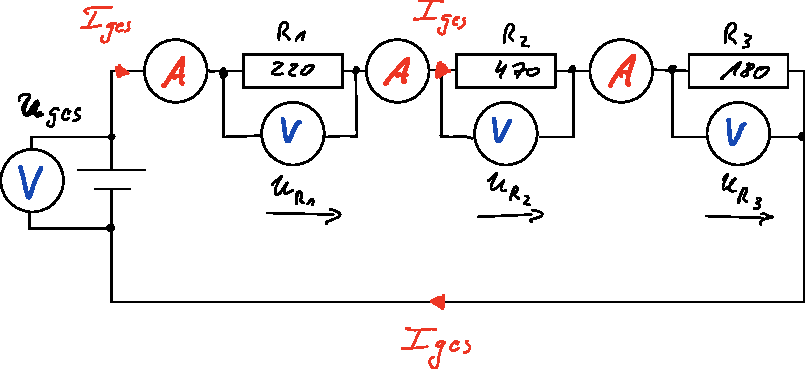
\includegraphics[width=0.6\textwidth]{images/Skizze/07_Reihenschaltung_Widerstaende_Skizze.pdf}
\caption{Reihenschaltung - Widerstände}
%\label{fig:}%% anpassen
\end{figure}

Spannungsteilerschaltung, an den einzelnen Widerständen fällt
individuell eine Spannung ab. Alle Einzelspannungen zusammen addiert
ergibt die Gesamtspannung.

Der Strom bleibt konstant.

\newpage

\section{Innenwiderstand von
Spannungsquellen}\label{innenwiderstand-von-spannungsquellen}

\begin{figure}[!ht]% hier: !ht
\centering
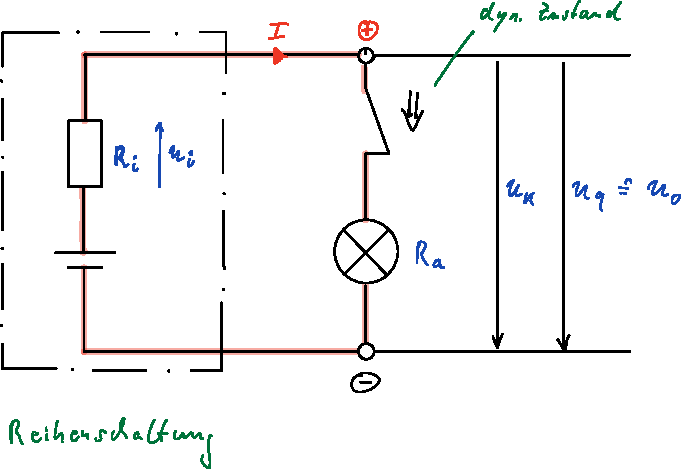
\includegraphics[width=0.6\textwidth]{images/Skizze/14_ Innenwiderstand_von_Spannungsquellen_Skizze.pdf}
\caption{Innenwiderstand von Spannungsquellen}
%\label{fig:}%% anpassen
\end{figure}

\begin{table}[!ht]% hier: !ht 
\centering 
	\caption{}% \label{tab:}%% anpassen 
\begin{tabular}{@{}lll@{}}
\hline
\textbf{Bezeichnung} & \textbf{Benennung} & \textbf{Einheit} \\
\hline
$U_q$ & Quellspannung & $[V]$ \\
$U_0 (U_{Null})$ & Leerlaufspannung & $[V]$ \\
$U_k$ & Klemmenspannung (Last, mit Verbraucher) & $[V]$ \\
$U_i$ & Spannungsabfall am Innenwiderstand & $[V]$ \\
$R_i$ & Innenwiderstand & $[\Omega]$ \\
$R_a$ & Außenwiderstand & $[\Omega]$ \\
$I$ & Stromfluss, -stärke & $[A]$ \\
\hline
\end{tabular} 
\end{table}

Ist der Gesamtwiderstand aller Zellen, ist auch Temperaturabhängig.

Die Klemmenspannung unter Last ist um Spannungsfall niedriger als die
Leerlaufspannung.

$\boxed{U_k = U_q - I \cdot R_i} \quad [V - A \cdot \Omega \to V - V] = V$

$\boxed{R_i = \frac{U_i}{I}} \quad \boxed{U_k = U_q - U_i - U_v} \quad \boxed{R_{ges} = R_i + R_l + R_\text{ü} + R_{La}}$

\newpage

\section{Relais}\label{relais}

Mit einem kleinen Steuerstrom kann ich einen hohen Laststrom schalten.

Wird unterschieden zwischen Schließer-, Öffner- und Wechselrelais.

\begin{figure}[!ht]% hier: !ht
\centering
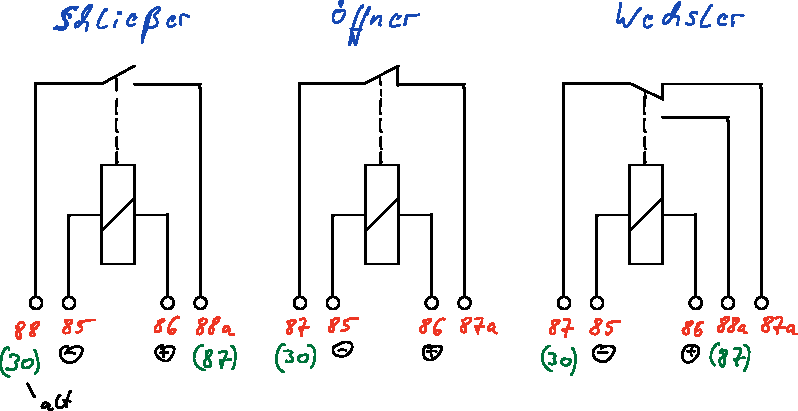
\includegraphics[width=0.7\textwidth]{images/Skizze/08_Relais_Skizze.pdf}
\caption{Relais}
%\label{fig:}%% anpassen
\end{figure}

\textbf{Ströme einer Relaisschaltung}

\begin{figure}[!ht]% hier: !ht
\centering
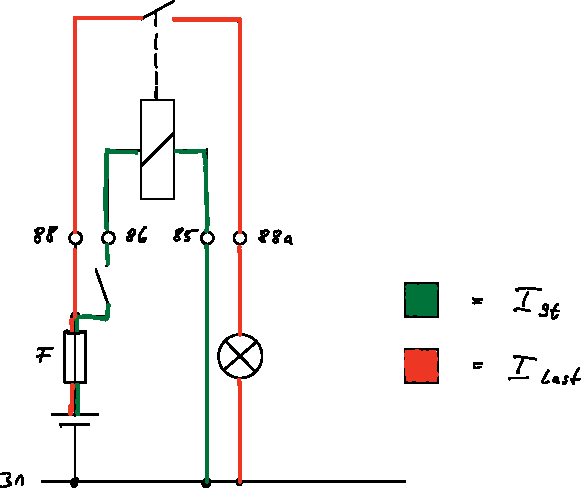
\includegraphics[width=0.4\textwidth]{images/Skizze/09_Stroeme_einer_Relaisschaltung_Skizze.pdf}
\caption{Ströme einer Relaisschaltung}
%\label{fig:}%% anpassen
\end{figure}

\begin{itemize}
\item
  \emph{Steuerstrom:} $50 - 200~mA$
\item
  \emph{Laststrom:} nach Verbraucher und Hersteller
\item
  \emph{Relaisspulenwiderstand:} $50 - 100~\Omega$ (ohne
  Schutzbeschaltung)
\end{itemize}

\newpage

\section{Parallelschaltung von
Widerständen}\label{parallelschaltung-von-widerstaenden}

\begin{figure}[!ht]% hier: !ht
\centering
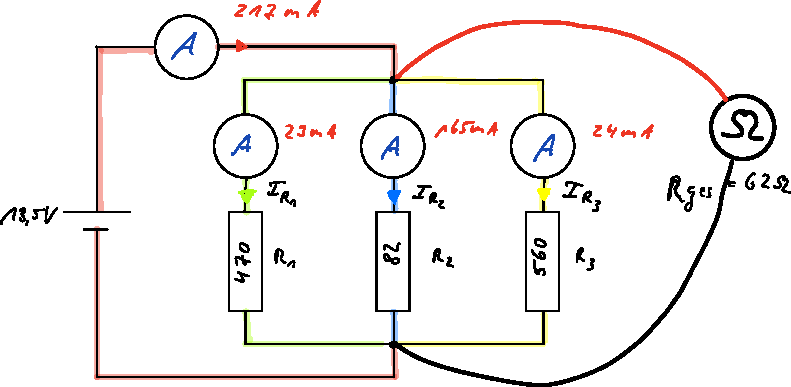
\includegraphics[width=0.6\textwidth]{images/Skizze/19_Parallelschaltung_Widerstaende_Skizze.pdf}
\caption{Parallelschaltung von Widerstände}
%\label{fig:}%% anpassen
\end{figure}

Stromteilerschaltung, der abfallende Einzelstrom ergibt, addiert den
Gesamtstrom.

Der Gesamtwiderstand der Schaltung ist immer kleiner als der kleinste
Einzelwiderstand.

Spannung ist überall gleich.

Ersatzwiderstand

$\boxed{R_{ges} = \frac{R_{Teil}}{n}}$

n = Anzahl der Widerstände (gleich große Widerstände)

$\boxed{R_{ges} = \frac{R_1 \cdot R_2}{R_1 + R_2}} \quad R_{ges} = \frac{1}{\frac{1}{R_1} + \frac{1}{R_2} + \frac{1}{R_3}}$

$\to R_{1} = \frac{1}{\frac{1}{R_{ges}} - \frac{1}{R_2} - \frac{1}{R_3}} \quad \to R_{2} = \frac{1}{\frac{1}{R_{ges}} - \frac{1}{R_1} - \frac{1}{R_3}} \quad \to R_{3} = \frac{1}{\frac{1}{R_{ges}} - \frac{1}{R_1} - \frac{1}{R_2}}$

\section{Leistung}\label{leistung}

Leistung ist das Produkt aus Spannung und Strom.

Mit 1 Volt Spannung und 1 Ampere Strom haben wir 1 Watt Leistung.

$\boxed{P = U \cdot I} \quad [V \cdot A] = W \quad \boxed{P = \frac{U^2}{R}} \quad \boxed{P = R \cdot I^2}$

\textbf{Lampe} $12~V/55~W$

$R_{La} = \frac{U^2}{P} \quad I_{tat} = \frac{U_k}{R_{La}} = \frac{U_{ges} - U_v}{R_{La}} \quad P_{tat} = U_k \cdot I_{tat}$

\newpage

\section{Spannungsverlust,
Spannungsfall}\label{spannungsverlust-spannungsfall}

Nennquerschnitt Tabellenbuch (\textcite{bell:2021:tabellenbuchKfz} S. 280)

Klemmbezeichnung Tabellenbuch (\textcite{bell:2021:tabellenbuchKfz} S. 273)

Spannungsfall Tabellenbuch (\textcite{bell:2021:tabellenbuchKfz} S. 280)

\begin{figure}[!ht]% hier: !ht
\centering
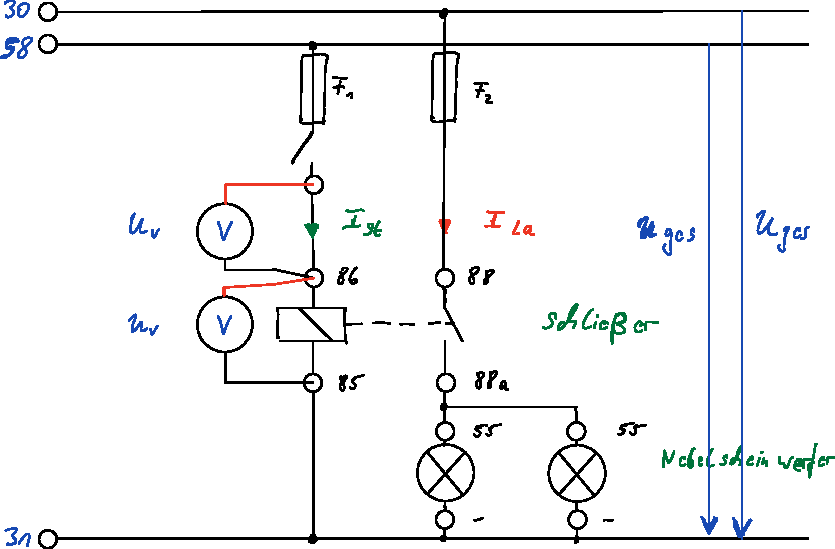
\includegraphics[width=0.65\textwidth]{images/Skizze/13_Spannungsverlust_Skizze.pdf}
\caption{Spannungsverlust}
%\label{fig:}%% anpassen
\end{figure}

\begin{table}[!ht]% hier: !ht 
\centering 
	\caption{}% \label{tab:}%% anpassen 
\begin{tabular}{@{}lll@{}}
\hline
\textbf{Bezeichnung} & \textbf{Benennung} & \textbf{Einheit} \\
\hline
$U_{ges}$ & Gesamtspannung & $[V]$ \\
$U_v$ & Spannungsverlust & $[V]$ \\
$U_k$ & Klemmspannung & $[V]$ \\
$R_l$ & Leiterwiderstand & $[\Omega]$ \\
$I$ & Stromfluss, Stromstärke & $[A]$ \\
\hline
\end{tabular} 
\end{table}

Spannungsverlust in einem stromdurchflossenen Leiter entsteht in Folge
des Leiterwiderstandes, der sich am Verbraucher als Verlust auswirkt.

$U_{ges} = U_v + U_k \quad U_v = R_l \cdot I \quad U_k = U_{ges} - R_l \cdot I$

$\boxed{U_v = \frac{\rho \cdot l \cdot I}{A}} \quad \bigl[\frac{\Omega \cdot mm^2 \cdot m \cdot A}{m \cdot mm^2}\bigl] = V \quad \rho_{Cu} = 0,0178~\frac{\Omega \cdot mm^2}{m} \quad \boxed{U_{v_{max}} = 0,5~V}$

\newpage

\section{Potenzialbestimmung}\label{potenzialbestimmung}

\begin{figure}[!ht]% hier: !ht
\centering
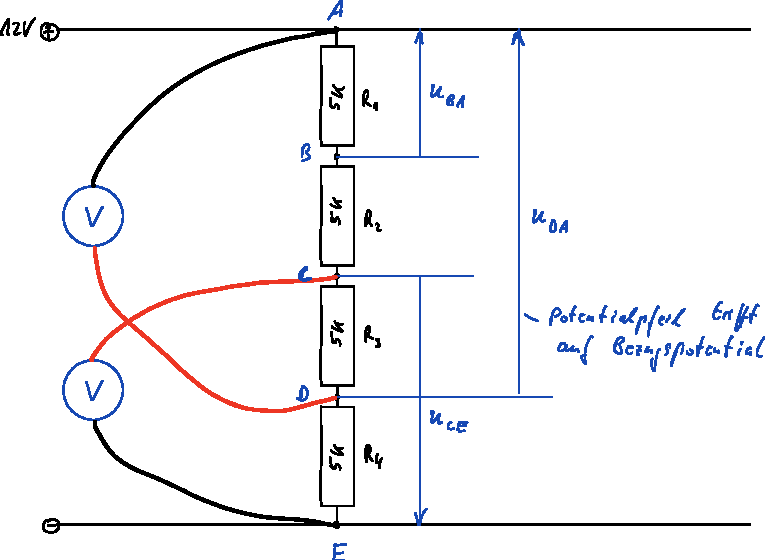
\includegraphics[width=0.6\textwidth]{images/Skizze/28_FT_Potentialbestimmung.pdf}
\caption{Potentialbestimmung}
%\label{fig:}%% anpassen
\end{figure}

Klemmenspannung und Potential

\begin{itemize}
\item
  $U_{R_1} = 3~V$, $U_{R_3} = 3~V$
\item
  $U_{CE} = 6~V$, $U_{BA} = -3~V$, $U_{DA} = -9~V$
\end{itemize}

Möchte man das/ein Potential an einem Punkt in einem Stromkreis
messen/bestimmen, bezieht man sich immer auf ein Bezugspotenzial. Die
Schreibweise dieser Messung lautet dann zum Beispiel $U_{CE}$, hierbei
möchte ich also das Potential C messen, C ist der erste Buchstabe, an
ihm wird der \emph{rote Clip} des Multimeters angeschlossen. Das
Bezugspotenzial hierbei E ist der zweite Buchstabe, hier wird
grundsätzlich der \emph{schwarze Clip} des Multimeters angeschlossen.
Potentialbestimmungen können auch zeichnerisch dargestellt werden.
Hierbei lautet die Vereinbarung, die Pfeilspitze des Spannungs- oder
Potentialpfeils trifft immer auf das Bezugspotenzial. Beispiel
$U_{DA}$.

\newpage

\section{Brückenschaltung -
Brückenspannung}\label{brueckenschaltung-brueckenspannung}

\begin{figure}[!ht]% hier: !ht
\centering
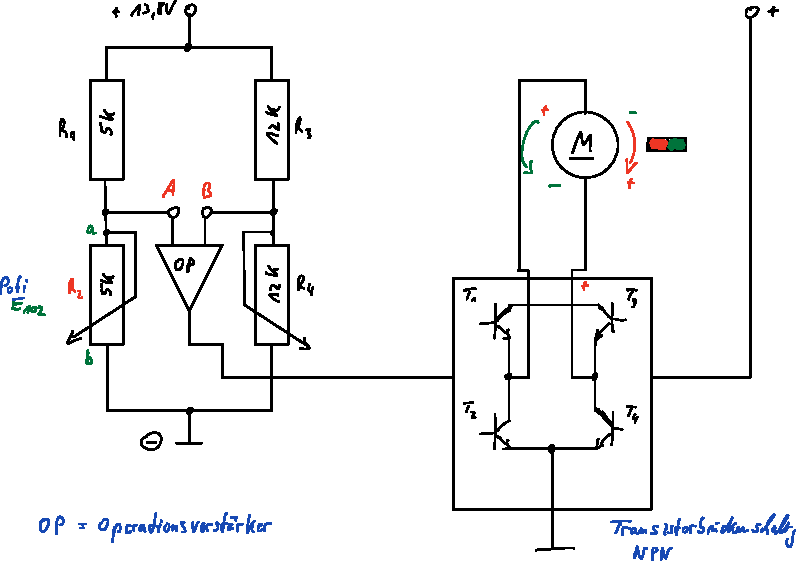
\includegraphics[width=0.6\textwidth]{images/Skizze/28_FT_Brueckenschaltung.pdf}
\caption{Brückenschaltung}
%\label{fig:}%% anpassen
\end{figure}

$U_{A\text{-}} = 6,9~V$, $U_{B\text{-}} = 6,9~V$, $U_{AB} = 0~V$
(keine Differenz)

$U_{A\text{+}} = -6,9~V$, $U_{B\text{+}} = -6,9~V$, $U_{AB} = 0~V$
(keine Differenz)

Poti $\to R_2 = 1~k$

$I_{Li} = \frac{U_{ges}}{R_{{Li}_{ges}}} = \frac{U_{ges}}{R_1 + R_2} = \frac{13,8}{5000 + 1000} =0,0023~A$

$U_{R_1} = R_1 \cdot I_{Li} = 5000~\Omega \cdot 0,0023~A = 11,5~V$

$U_{A\text{+}} = -11,5~V$, $U_{B\text{+}} = -6,9~V$,
$U_{AB} = -4,6~V$

$I_{Re} = \frac{U_{R_3}}{R_3} = \frac{11,5}{12000} =0,00096~A$

$R_4 = \frac{U_{R_4}}{I_{Re}} = \frac{U_{ges} - U_{R_3}}{I_{Re}} = \frac{13,8 - 11,5}{0,00096} = 2395,83~\Omega$

\chapter{Sensoren und Aktoren}
%ju 17-Sep-22 02-Sensoren-und-Aktoren.tex
\textbf{Sensoren} erfassen physikalische Effekte (Druck, Temperatur) und
wandeln diese in elektrische Signale um. (Sinne des Autos)

\textbf{Aktoren} wandeln elektrische Spannungssignale in physikalische
Effekte um (Stellglieder, Ausführen).

\section{Pulsweitenmodulation}\label{pulsweitenmodulation}

\begin{enumerate}
\item
  \textbf{PWM-Signal:} Rechtecksignal (vgl. Kennlinie)
\item
  \textbf{Messen:} Oszilloskop
\item
  \textbf{Ansteuerung:} $0 - 100~\%$, Impuls-Pause-Verhältnisänderung
  (nur Pulsweite ändert sich), aber Periodendauer / Frequenz bleibt
  konstant (keine Spannungsänderung!)
\item
  \textbf{Anwendung}

  \begin{itemize}
  \item
    Elektromotor (Drehzahl)
  \item
    Glühlampen (Helligkeit, dimmen)
  \item
    Beleuchtung, Beispiel: Einfaden-Glühlampe (Standlicht + Bremslicht)
  \end{itemize}
\end{enumerate}

Die \textbf{Pulsweitenmodulation} (PWM) ist eine digitale
Modulationsart, bei der eine technische Größe zwischen zwei Werten
(Spannungspegel $0~V$ und VCC) wechselt. Dabei wird bei konstanter
Frequenz ein Rechtecksignal moduliert, das in Pulsweite (\emph{oder}
Breite bzw. Länge) variiert. Das Verhältnis zwischen Impuls und Pause
(Ein- und Ausschaltzeit) wird als \textbf{Tastgrad / Tastverhältnis}
bezeichnet. \textbf{Anwendung} in der Steuer- und Regelungstechnik.

\section{Halbleiter}\label{halbleiter}

\textbf{Halbleiter} ist ein kristalliner Stoff, der sich bei tiefen
Temperaturen wie ein Isolator verhält und bei höheren Temperaturen nimmt
die elektrische Leitfähigkeit zu. Der Widerstand ist temperaturabhängig.

\textbf{Halbleiterwerkstoffe}

\begin{itemize}
\item
  \textbf{Metalle} Beispiel: Eisen, Kupfer
\item
  \textbf{Isolierstoffe} Beispiel: Kunststoff
\item
  \textbf{Halbleitermaterial} Beispiel: reines Silizium / Germanium
  \textbf{Anwendung} Beispiel: Diode, Transistor
\end{itemize}

\textbf{Dotieren} reines Silizium / Germanium wird verunreinigt, um die
elektrische Leitfähigkeit zu verbessern.

\textbf{P-Leiter und N-Leiter}

\begin{enumerate}
\item
  \textbf{P-Leiter} entsteht, wenn das Leitermaterial Silizium
  verunreinigt wird mit Bohr und bei \emph{Elektronenmangel} enthält es
  freie positive Ladungen. Löcherstrom
\item
  \textbf{N-Leiter} entsteht, wenn das Leitermaterial Silizium
  verunreinigt wird mit Phosphor und bei \emph{Elektronenüberschuss}
  enthält es freie negative Ladungen. Elektronenstrom
\end{enumerate}

$\to$ Legt man an den Halbleiterkristall eine elektrische Spannung an,
dann kommt es zum Elektronenfluss, weil die Elektronen versuchen sich
auszugleichen.

\section{Halbleiterwiderstände NTC und
PTC}\label{halbleiterwiderstaende-ntc-und-ptc}

\begin{enumerate}
\item
  \textbf{Heißleiter} $\to$ NTC-Widerstände bis $250^\circ\text{C}$

  \begin{itemize}
  \item
    \emph{negativer Temperatur-Koeffizient} $\to$ fallender Widerstand
    bei steigender Temperatur $\uparrow \downarrow$
  \item
    vgl. Kennlinie (x = Temperatur, y = Widerstand)
  \item
    \textbf{Anwendung:} Temperatursensoren (Kühlmittel-, Kraftstoff-,
    Luft-, Motortemperaturfühler)
  \item
    Schaltsymbol
  \item
    typische Werte: Kalt: $2 - 4~k\Omega$ und Warm:
    $200 - 400~\Omega$
  \item
    \emph{Leitfähigkeit} steigt mit zunehmender Temperatur
  \item
    Widerstand und Spannungsfall am NTC werden kleiner
  \end{itemize}
\item
  \textbf{Kaltleiter} $\to$ PTC-Widerstände bis
  $950 - 1000^\circ\text{C}$

  \begin{itemize}
  \item
    \emph{positiver Temperatur-Koeffizient} $\to$ zunehmender
    Widerstand bei steigender Temperatur $\uparrow \uparrow$
  \item
    vgl. Kennlinie (x = Temperatur, y = Widerstand)
  \item
    \textbf{Anwendung:} Hochtemperaturbereich
    (Diesel-Abgastemperatursensoren), Glühkerzen, Heizungen von
    Lambdasonden
  \item
    Schaltsymbol
  \item
    \emph{Leitfähigkeit} verringert sich mit zunehmender Temperatur
  \item
    Widerstand und Spannungsfall am PTC werden größer
  \item
    >>Je höher der Widerstand, desto geringer der Stromfluss.<<
  \end{itemize}
\end{enumerate}

\chapter{Hochvolt}
%ju 13-Aug-22 03-Hochvolt.tex
\textbf{Reichweite Batterie} $\sim 770~km$ (MERCEDES EQS (2021) -
S-KLASSE \footnote{\url{https://www.auto-motor-und-sport.de/})} (Stand:
Mai/2022)

\textbf{Spannung Bordnetz} $400~V - 800~V$ (Porsche Taycan, Audi
e-tron)

\textbf{Batterie laden} 1-Phase ($3,7~Km$), 3-Phasen, Gleichstrom

\section{Was sind HV-eigensichere
Fahrzeuge?}\label{was-sind-hv-eigensichere-fahrzeuge}

Gewährleisten einen vollständigen Berühr- und Lichtbogenschutz gegenüber
HV-System.

\begin{itemize}
\item
  System überwacht sich selbst
\item
  Serienfahrzeug
\item
  Sicherheitslinie (Pkw)

  \begin{itemize}
  \item
    \textbf{Außer:} Lkw, Busse, Eigenbau (Vorsicht beim Umrüsten und
    Nachrüsten), Unfallfahrzeug
  \end{itemize}
\end{itemize}

\textbf{IT-Netz} IT steht für isoliert und Terra (von der Erde
isoliertes System): Das HV-System ist sowohl wechsel- als auch
gleichstromseitig von der Fahrzeugmasse galvanisch getrennt oder
isoliert.

\section{Qualifikationsstufen}\label{qualifikationsstufen}

Jeder \textbf{Gewerbetreibende} benötigt die Stufe-S, um ein HV-Fahrzeug
bewegen zu dürfen.

\textbf{Unterweisung} einmal jährlich für Gesellen und halbjährlich für
Lehrlinge. $\to$ Person sensibilisieren auf jedes Fahrzeug einzeln.

\textbf{Wie heißt die neue Sicherheitsverordnung?}

DGUV 209-093 (Deutsche gesetzliche Unfallversicherung) Qualifizierung
für Arbeiten an Fahrzeugen mit HV-Systemen.

\textbf{Qualifikationsstufen}

\begin{itemize}
\item
  \textbf{Stufe S} sensibilisierte Person (Bedienen von Fahrzeugen mit
  HV-System)
\item
  \textbf{Stufe 1S} Fachkundige unterwiesene Person (Motto: Hände weg
  von Orange!)
\item
  \textbf{Stufe 2S} fachkundige Person (alle arbeiten, aber nicht unter
  Spannung, Freischalten)
\item
  \textbf{Stufe 3S} fachkundige Person -- für Arbeiten unter Spannung
  stehenden HV-System (Energiespeicher öffnen)
\end{itemize}

\textbf{Welche Qualifikationen sind für folgende Arbeiten notwendig?}

\begin{enumerate}
\item
  \textbf{VW E-Golf kommt zum Räderwechsel}

  \begin{itemize}
  \item
    Fachkundige unterwiesene Person
  \end{itemize}
\item
  \textbf{Lehrling soll VW E-Golf in eine andere Filiale fahren}

  \begin{itemize}
  \item
    Sensibilisierte Person
  \end{itemize}
\item
  \textbf{Beim Smart ED soll der Klimakompressor getauscht werden}

  \begin{itemize}
  \item
    Fall 1: Wenn nicht freigeschaltet ist $\to$ Stufe 2S
  \item
    Fall 2: Wenn freigeschaltet ist $\to$ Stufe 1S + Klimaschein
  \end{itemize}
\item
  \textbf{Tesla Model S braucht eine neue HV-Batterie}

  \begin{itemize}
  \item
    Fachkundige Person
  \end{itemize}
\item
  \textbf{Nach Unfall lässt sich Mercedes Vito E-Cell nicht mehr über
  Service-Disconnect-Stecker spannungsfrei schalten}

  \begin{itemize}
  \item
    Fachkundige Person -- für Arbeiten unter Spannung stehenden
    HV-System
  \end{itemize}
\end{enumerate}

\section{Erkläre das Freischalten des
HV-Systems?}\label{erklaere-das-freischalten-des-hv-systems}

Kunde kommt mit E-Auto in die Werkstatt. Was passiert jetzt?

Beginn Gefahrübergang: mit Schlüsselübergabe + Werkstattauftrag
unterschrieben

\begin{enumerate}
\item
  Hütchen mit Magnet aufs Dach $\to$ Achtung Hochspannung!
\item
  Fahrzeug in Werkstatt fahren
\item
  Abschranken

  \begin{itemize}
  \item
    im Abstand $1~m$ um das Fahrzeug herum
  \item
    Gefahren absperren: Bedeutung von gelb/schwarzes Band - langfristig
    oder rot/weiß - kurzfristig
  \end{itemize}
\item
  rotes Schild auf die Windschutzscheibe kleben $\to$ Achtung
  Hochvolt! Nicht freigeschaltet, mit Namen und Telefonnummer
\item
  Zündung ausschalten und Zündschlüssel entfernen
\item
  Sicherheitshandschuhe prüfen und anziehen, Schutzbrille, lange
  Kleidung ohne Reißverschluss (Vgl. Körperwiderstand)
\item
  Minuspol der 12 V-Batterie abklemmen
\item
  Warten 5 Minuten $\to$ bis Kondensatoren sich entladen von Bordnetz
  und HV-System

  \begin{itemize}
  \item
    Sicherheitslinie wird geöffnet
  \item
    Trennrelais öffnen und schalten Spannung ab
  \item
    Kondensatoren entladen sich
  \end{itemize}
\item
  Service-Disconnect-Stecker der HV-Batterie abziehen, falls nicht
  vorhanden, Sicherheitslinie unterbrechen
\item
  Zündschlüssel und Disconnect-Stecker wegschließen (mind. 10 m
  Entfernung) und sichern gegen wieder einschalten
\item
  Messen mit dem Duspol

  \begin{itemize}
  \item
    Messgerät überprüfen: Hochspannungsbereich 230 V-Steckdose,
    Niederspannungsbereich 12 V-Batterie
  \item
    Messung durchführen: am Inverter alle drei Phasen messen
  \item
    Messgerät überprüfen (gleiche Spannungsquellen):
    Hochspannungsbereich 230 V, Niederspannungsbereich 12 V-Batterie
  \item
    Spannungsfreiheit festgestellt
  \end{itemize}
\item
  Dokumentieren über das Freischalten (Was wurde gemacht? Wie wurde das
  Fahrzeug übergeben?)
\item
  weißes Schild auf die Windschutzscheibe kleben $\to$ Fahrzeug ist
  spannungsfrei, Fahrzeug gegen Wiedereinschalten gesichert, mit Namen
  und Telefonnummer
\item
  Jetzt kann gearbeitet werden.
\end{enumerate}

Pilotlinie, Interlock, Sicherheitslinie (Niedervolt)

\textbf{Wie hoch ist der Körperwiderstand ab einer Spannung von 100 V?}

Berührung der beiden Batteriepole

\begin{itemize}
\item
  $1000~\Omega$ von Hand-zu-Hand oder Hand-zu-Fuß
\item
  $450~\Omega$ von Hand-zu-Brust
\item
  $\text{Körperstrom} = \frac{400~V}{1000~\Omega} = 400~mA$ der
  absolut tödlich wäre.
\end{itemize}

Ein Strom von beispielsweise $50~mA$ kann zur Muskelverkrampfung
führen, sodass sich die Person nicht mehr selbstständig von der
Spannungsquelle lösen kann. Schon nach wenigen Sekunden könnte es auch
bei niedrigen Strömen zu tödlichen Unfällen kommen. (Einwirkzeit)

\textbf{Sicherheitshandschuhe prüfen} (rot, bis $1000~V$, vor jedem
Freischalten)

\begin{itemize}
\item
  Handschuh aufdrehen und auf Dichtheit prüfen oder Prüfgerät
\item
  keine Verfärbung oder Punkte
\item
  Aufdruck vollständig
\end{itemize}

\chapter{Generator}
%ju 16-Dez-22 04-Generator.tex
\textbf{Drehstromgenerator / Lichtmaschine / Generator}

Quelle: Fabian Lindenberg, Kfz-Technik einfach erklärt \footnote{\url{https://www.youtube.com/watch?v=O7ydsAZ6bes}}

\section{Komponenten}\label{komponenten}

\begin{enumerate}
\item
  \textbf{Regler} (Multifunktionsregler hat keine Erregendioden, bekommt
  Spg. von Kl.30)
\item
  \textbf{Schleifringe}
\item
  \textbf{Gleichrichterdioden} (Leistungsdioden)
\item
  \textbf{Klauenpolläufer} (mit Riemenscheibe $\to$ Antrieb Motor und
  Schleifringe $\to$ Regler)
\item
  \textbf{Erregerwicklung} (Rotor, dreht sich, sitzt im Klauenpolläufer)
\item
  \textbf{Ständerwicklung} (mit Gehäuse, Stator, steht)
\item
  \textbf{Lüfter}
\end{enumerate}

\textbf{Diodenplatte:} 6x Gleichrichterdioden (3x Plusdioden, 3x
Minusdioden), 3x Erregerdioden

\textbf{Klauenpolläufer} 12 Pole (je 6 Nord- und Südpole) x 3
Statorspulen = 36 Halbwellen = 1x Umdrehung. Batterie und Kondensator
glättet die Gleichspannung.

\begin{figure}[!ht]% hier: !ht
\centering
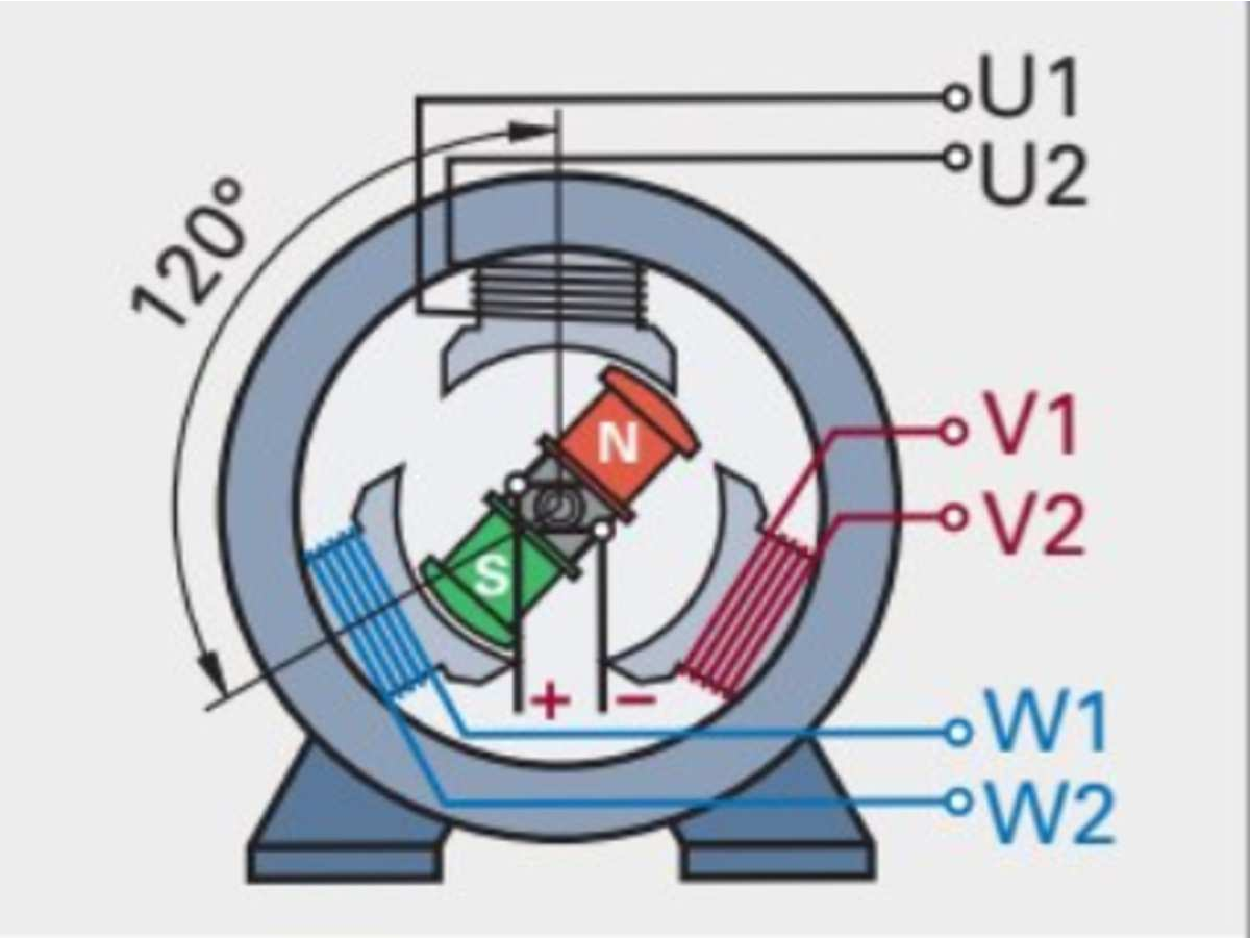
\includegraphics[width=0.4\textwidth]{images/Generator/Generator-11.pdf}
\caption{Generatoraufbau - Drei Ständerwicklungen U,V,W und ein Polrad}
%\label{fig:}%% anpassen
\end{figure}

\begin{figure}[!ht]% hier: !ht
\centering
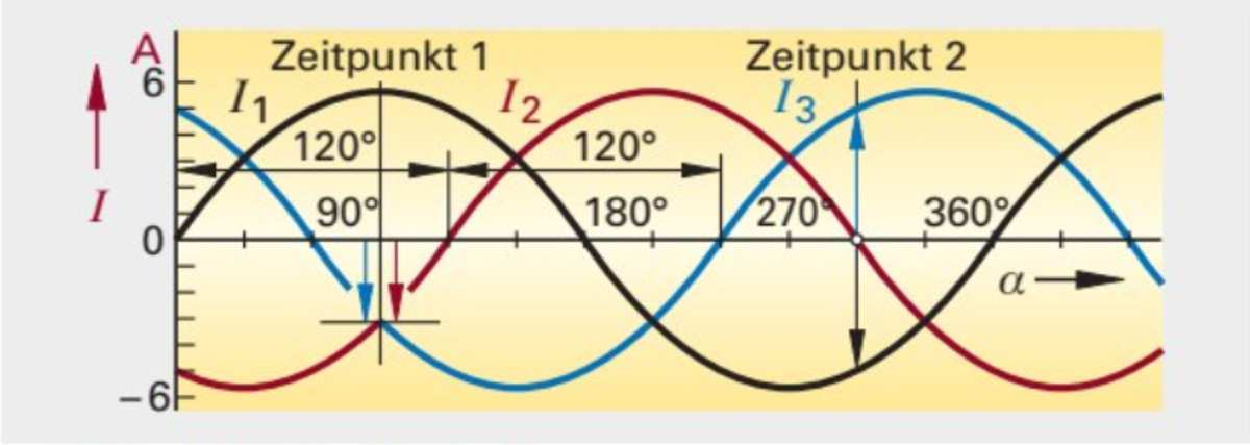
\includegraphics[width=0.4\textwidth]{images/Generator/Generator-8.pdf}
\caption{3 Wechselspannungen mit 120° Phasenverschiebung}
%\label{fig:}%% anpassen
\end{figure}

\section{Multifunktionsregler}\label{multifunktionsregler}

\begin{figure}[!ht]% hier: !ht
\centering
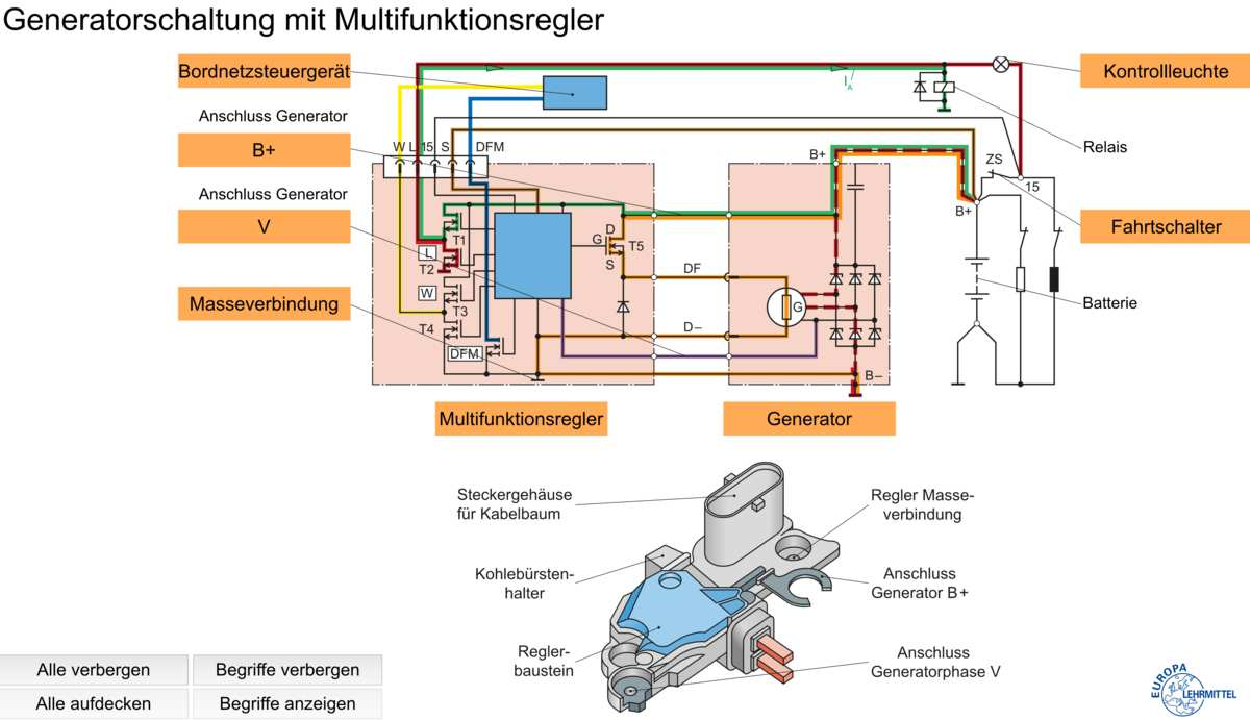
\includegraphics[width=0.85\textwidth]{images/Generator/Generator-1.pdf}
\caption{Schaltung Generator mit Multifunktionsregler, Quelle:
Europa-Verlag}
%\label{fig:}%% anpassen
\end{figure}

\textbf{Merkmale}

\begin{enumerate}
\item
  Unterstützung Motormanagement
\item
  Batterieüberwachung
\item
  Auslastungsüberwachung
\item
  Temperaturabhängige Ladespannung
\item
  Schutz gegen Überlastung / Kurzschluss
\item
  Interne Fehlerdiagnose $\to$ SG
\item
  Vorerregerstrom Steuern (Dreht sich der Generator)
\item
  Low-Response (Start \& Fahrt: Belastung des Generators wird verzögert
  zugeschaltet, Kraftstoff sparen)
\end{enumerate}

\newpage

\section{Generator prüfen}\label{generator-pruefen}

\textbf{Ladekontrolle an}

\begin{itemize}
\item
  Zündung an, Motor steht
\item
  Erregungsunterbrechung
\item
  Überspannung
\item
  Keilriemen gerissen
\item
  Leitungsunterbrechung
\item
  Defekte Masseverbindung
\end{itemize}

\textbf{Generator Anschluss}

\begin{enumerate}
\item
  \textbf{W} Drehzahl
\item
  \textbf{B-} Masse
\item
  \textbf{D+} Ladekontrolle, Erregerwicklung
\item
  \textbf{B+} Batterie
\item
  \textbf{DF} Regler, Erregerwicklung
\end{enumerate}

\textbf{Generator mit Multifunktionsregler Anschluss}

\begin{enumerate}
\item
  \textbf{L} Ladekontrollleuchte
\item
  \textbf{S} Sense, Batterie überwachen
\item
  \textbf{W} Drehzahlsignal zur Regelung des Vorerregerstroms
\item
  \textbf{V} Phasenspannung überwachen (Fehlerdiagnose, Beispiel: def.
  Keilriemen erkennen)
\item
  \textbf{DFM} PWM-Signal des Erregerstroms zur Auslastung des
  Generators
\end{enumerate}

\textbf{Erregerspannung und Generatorspannung / Ladespannung messen}

\begin{itemize}
\item
  Unter Belastung (Verbraucher EIN)
\item
  Motordrehzahl (ca. 1800 - 2200 1/min)
\item
  \textbf{Erregerspannung}

  \begin{itemize}
  \item
    Messpunkt: (D+ und D-/B-/Masse)
  \end{itemize}
\item
  \textbf{Generatorspannung / Ladespannung}

  \begin{itemize}
  \item
    Messpunkt: (B+ und D-/B-/Masse)
  \end{itemize}
\end{itemize}

\textbf{Fehler}

\begin{enumerate}
\item
  Oberwelle normal
\item
  Minusseitig eine Sperrdiode defekt $\to$ Eine Welle wäre weg,
  Leistung von der Spule fehlt
\item
  Erregerdiode defekt $\to$ Ladespannung geht runter
\end{enumerate}

\begin{figure}[!ht]% hier: !ht
\centering
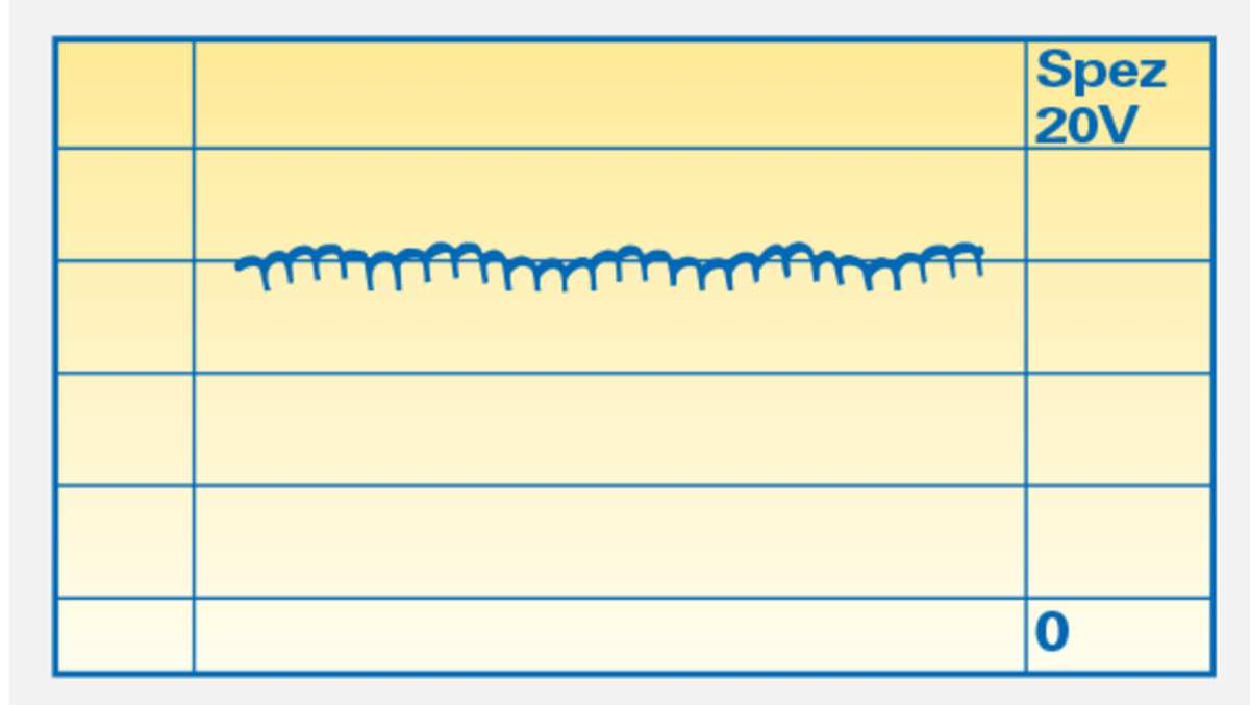
\includegraphics[width=0.4\textwidth]{images/Generator/Generator-2.pdf}
\caption{Generator Gutbild, Quelle: Europa-Verlag}
%\label{fig:}%% anpassen
\end{figure}

\begin{figure}[!ht]% hier: !ht
\centering
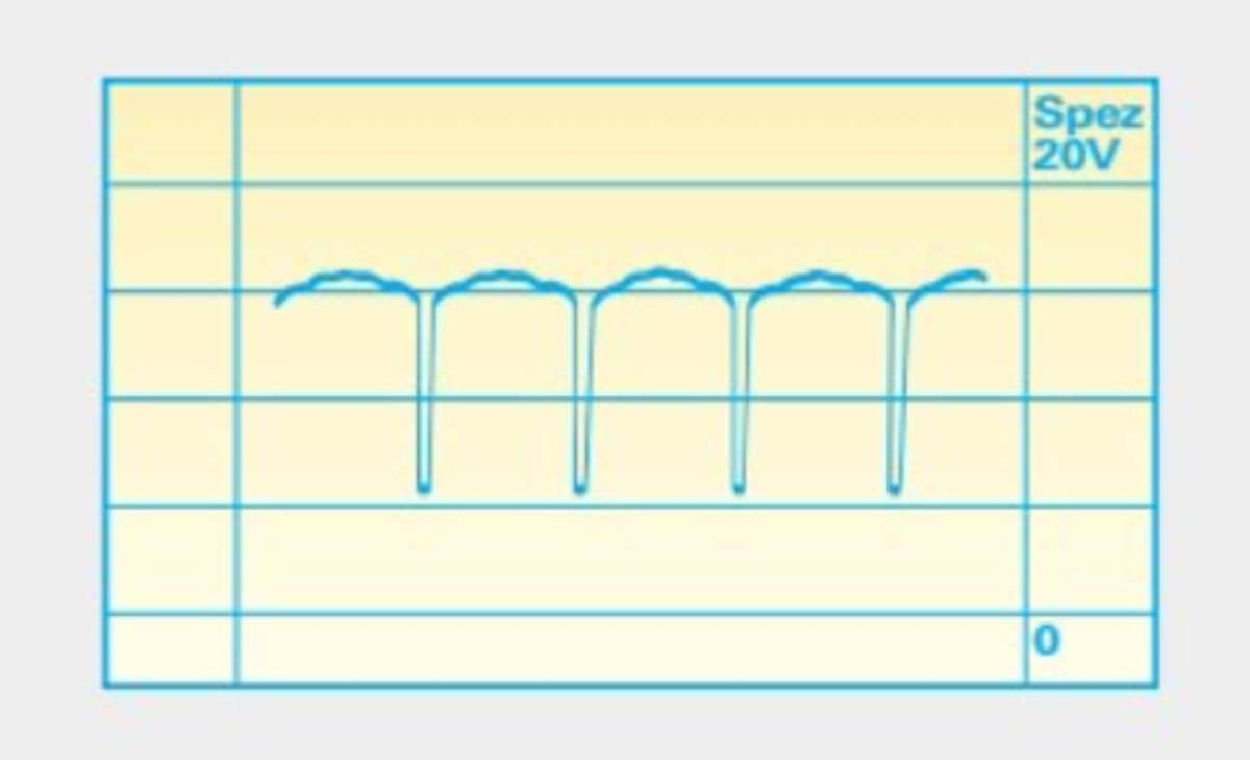
\includegraphics[width=0.4\textwidth]{images/Generator/Generator-5.pdf}
\caption{Generator Fehler - Unterbrechung einer Minusdiode, Quelle:
Europa-Verlag}
%\label{fig:}%% anpassen
\end{figure}

\newpage

\section{Energieumwandlung}\label{energieumwandlung}

kinetische Energie + elektrische Energie (Drehmoment) $\to$
\textbf{Generator} $\to$ elektrische Energie

\textbf{Induktion} mit ein Magnetfeld Elektronen bewegen.

Magnet (Nordpol/Südpol, anziehen / abstoßen)

Rechte-Handregel: Magnetfeld bestimmen

\begin{enumerate}
\item
  Stromdurchflossener Leiter $\to$ erzeugt Magnetfeld
\item
  Stromdurchflosse Spule $\to$ erzeugt großes Magnetfeld
\item
  Rotor (Erregerwicklung, Fremderregt) und Stator (mit 3x Spulen, U / V
  / W) $\to$ erzeugt drehbares Magnetfeld
\end{enumerate}

\textbf{indizierte Spannung} ist abhängig

\begin{enumerate}
\item
  Anzahl Wicklungen von Statorspulen
\item
  Drehzahl Generator
\item
  Stärke des Magnetfeldes
\item
  Fläche
\end{enumerate}

\begin{figure}[!ht]% hier: !ht
\centering
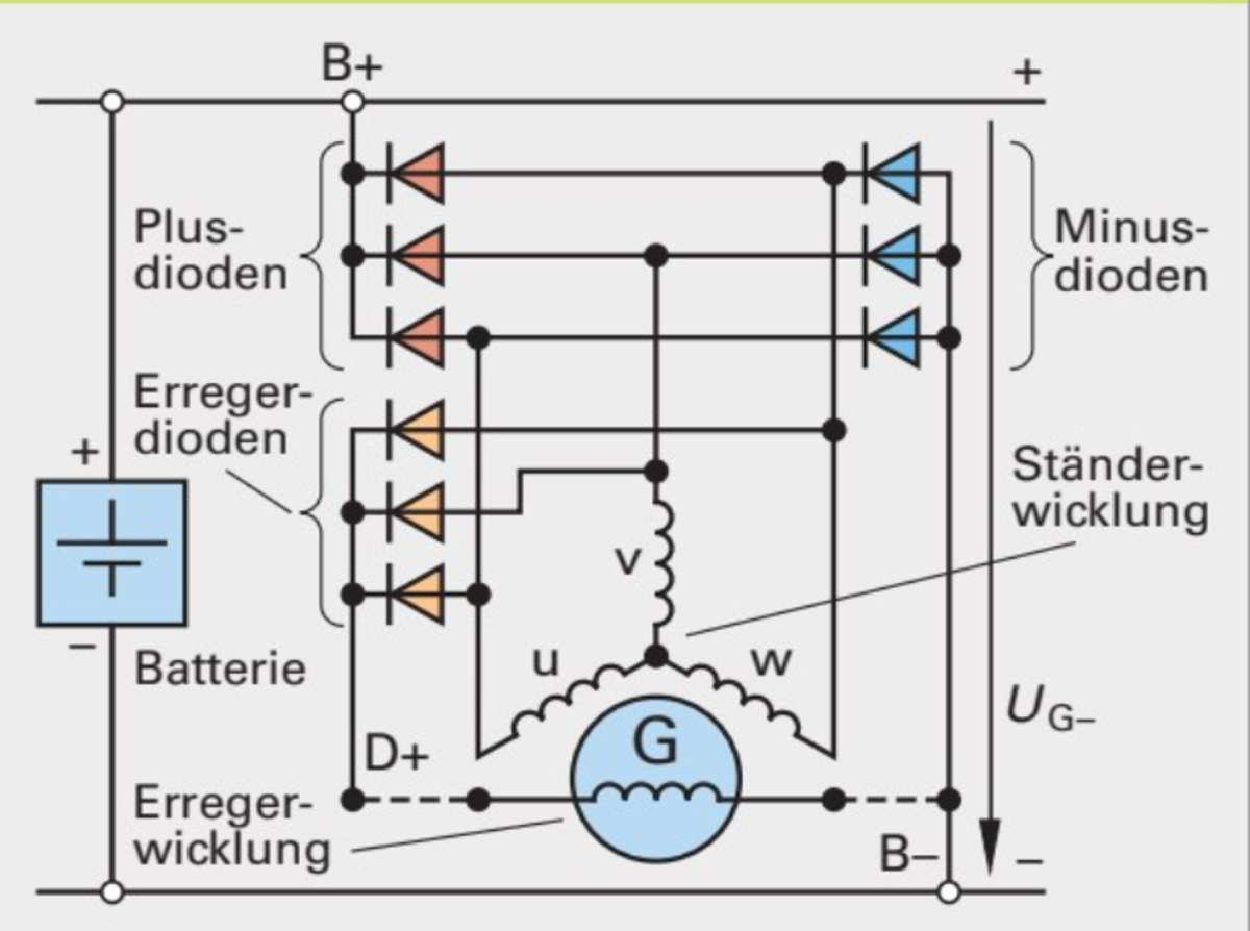
\includegraphics[width=0.3\textwidth]{images/Generator/Generator-6.pdf}
\caption{Drehstrom - Brückenschaltung}
%\label{fig:}%% anpassen
\end{figure}

\begin{figure}[!ht]% hier: !ht
\centering
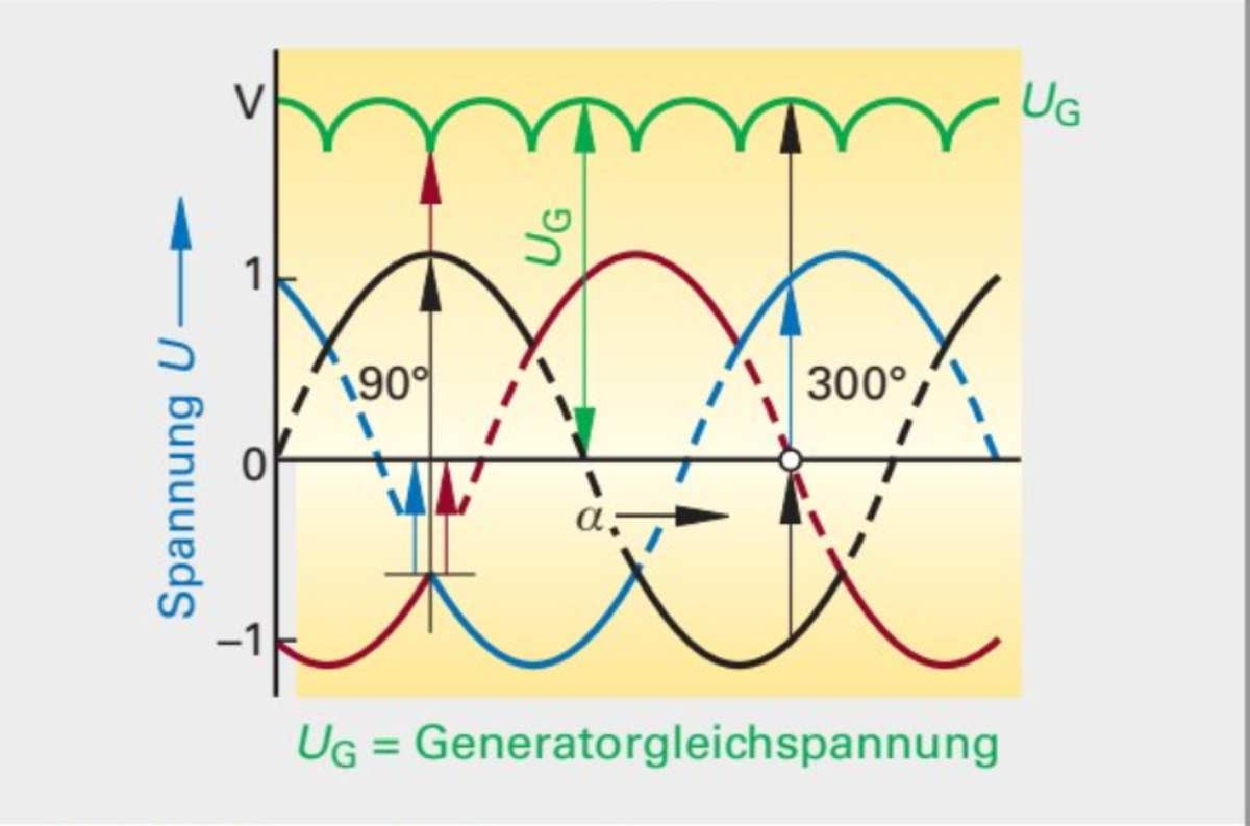
\includegraphics[width=0.3\textwidth]{images/Generator/Generator-7.pdf}
\caption{Gleichrichtung der Generatorspannung}
%\label{fig:}%% anpassen
\end{figure}

\newpage

\section{Energiefluss}\label{energiefluss}

\begin{figure}[!ht]% hier: !ht
\centering
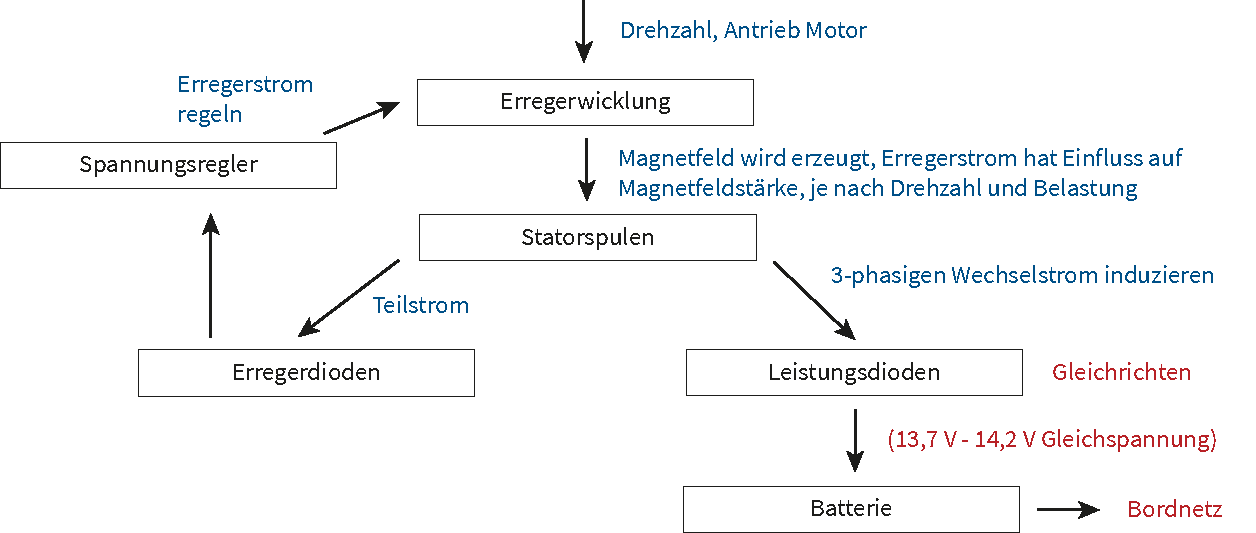
\includegraphics[width=0.8\textwidth]{images/Generator/Generator-Energiefluss.pdf}
\caption{Energiefluss}
%\label{fig:}%% anpassen
\end{figure}

\textbf{Erregerwicklung} sitzt im Klauenpolläufer, erzeugt Magnetfeld
welches auf die Statorspulen wirkt

\textbf{Statorspulen} Sternschaltung, Durch das Magnetfeld der
Erregerwicklung wird eine Spannung induziert. 3x Spulen um 120° versetzt
$\to$ 3-phasige Wechselspannung

\textbf{Leistungsdioden} Richten die 3-phasige Wechselspannung in eine
Gleichspannung um.

\textbf{Erregerdioden} Spannungsversorgung des Spannungsreglers.

\textbf{Spannungsregler} regelt den Erregerstrom und variiert damit die
Stärke des Magnetfeldes. \textbf{Ladespannung ist Konst.} bei allen
Motordrehzahlen (Leerlauf - Vollast) u. Belastungen (Verbraucher).
\textbf{Wie?} Je stärker das Magnetfeld, desto größer ist die Spannung
die in den Statorspulen induziert wird.

\newpage

\section{Schaltung}\label{schaltung}

\begin{figure}[!ht]% hier: !ht
\centering
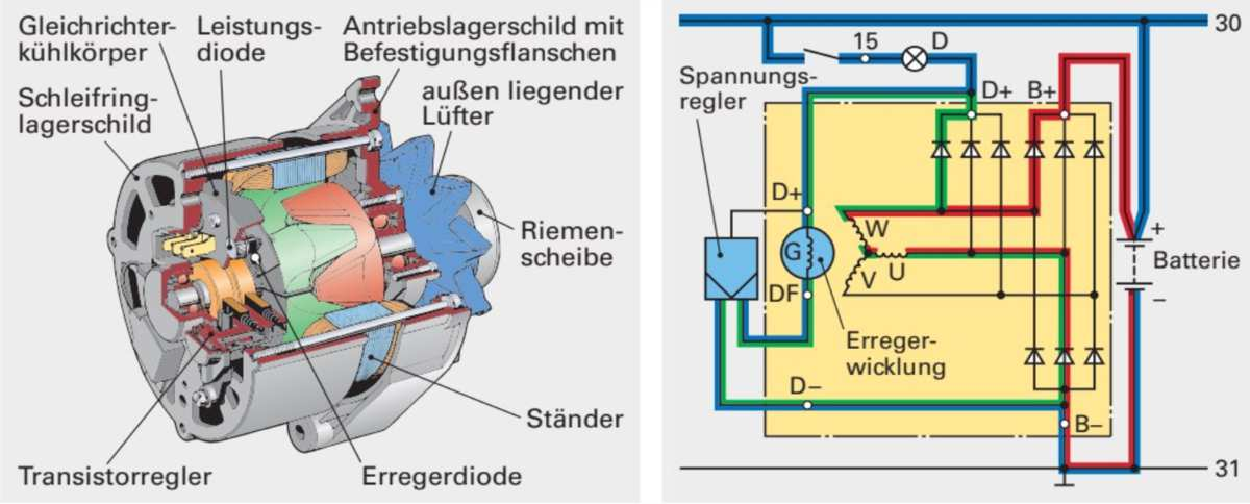
\includegraphics[width=0.85\textwidth]{images/Generator/Generator-9.pdf}
\caption{Schaltung Generator mit Transistorregler, Quelle:
Europa-Verlag}
%\label{fig:}%% anpassen
\end{figure}

Zündung an, Motor steht

\textbf{Vorerregerstromkreis (blau)} B+ $\to$ Fahrtschalter $\to$
Ladekontrolllampe $\to$ D+ $\to$ Erregerwicklung $\to$ Regler DF
$\to$ Masse $\to$ B-

Zündung an, Motor läuft

\textbf{Erregerstromkreis (grün)} Ständerwicklung $\to$ Erregerdioden
$\to$ D+ $\to$ Erregerwicklung $\to$ Regler DF $\to$ Regler D-
$\to$ Minusdioden $\to$ Ständerwicklung

\textbf{Ladestromkreis (rot)} Ständerwicklung $\to$ Plusdioden $\to$
B+ $\to$ Verbraucher $\to$ Masse $\to$ Minusdioden $\to$
Ständerwicklung

\newpage

\begin{figure}[!ht]% hier: !ht
\centering
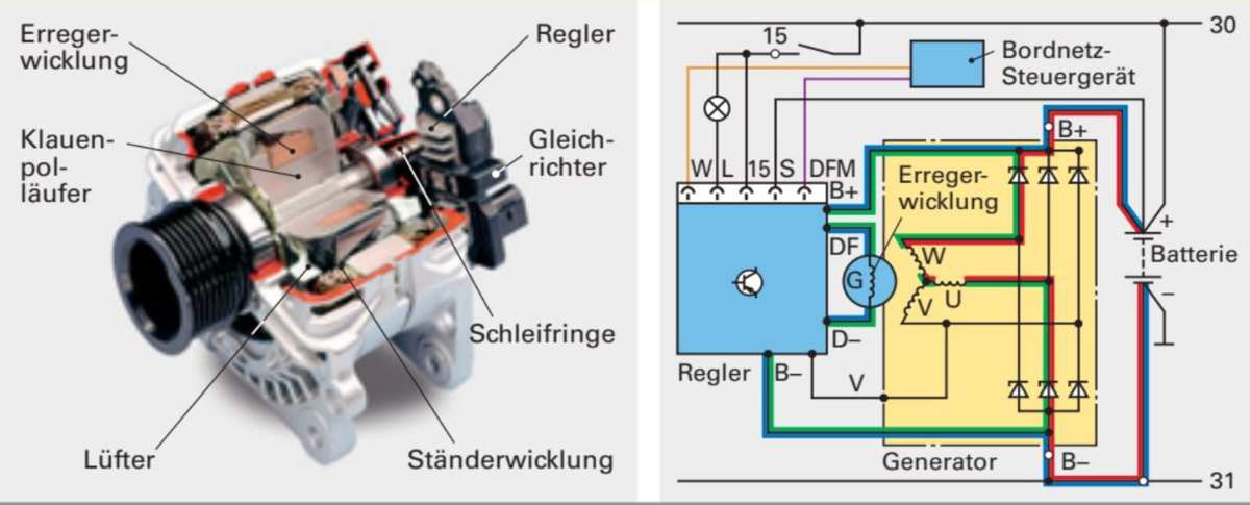
\includegraphics[width=0.85\textwidth]{images/Generator/Generator-10.pdf}
\caption{Schaltung Generator mit Multifunktionsregler, Quelle:
Europa-Verlag}
%\label{fig:}%% anpassen
\end{figure}

\textbf{Vorerregerstromkreis (blau)} B+ $\to$ Erregerwicklung $\to$
Regler DF $\to$ Reglerendstufe $\to$ B-

Zündung an, Motor läuft

\textbf{Erregerstromkreis (grün)} Ständerwicklung $\to$ Plusdioden
$\to$ Regler B+ $\to$ Regler DF $\to$ Erregerwicklung $\to$
Regler D- $\to$ Regler B- $\to$ Minusdioden $\to$ Ständerwicklung

\textbf{Ladestromkreis (rot)} Ständerwicklung $\to$ Plusdioden $\to$
B+ $\to$ Verbraucher $\to$ Masse $\to$ Minusdioden $\to$
Ständerwicklung

\chapter{Datenbus}
%ju 17-Sep-22 05-Datenbus.tex
Quelle: Fabian Lindenberg, Kfz-Technik einfach erklärt \footnote{\url{https://www.youtube.com/watch?v=0a33FFpn_eM\&list=PLJXzCsL6HEwzoI3j8tGLKUHjLx0gTxus8}}

\textbf{Früher} für jedes Signal eine Leitung $\to$ viele Kabel
notwendig, wenn mehrere Steuergeräte auf Sensordaten zugreifen wollen.

\textbf{Heute} ein Steuergerät liest die Sensordaten aus und schickt
diese auf den Datenbus. \emph{Beispiel} Motordrehzahlsignal wird von
folgenden Steuergeräten benötigt: Motor, Getriebe, Kombiinstrument,
Klimaanlage, ESP.

\textbf{Datenübertragung im Kfz} Ermöglicht den Transport und Austausch
von Informationen in Form von Daten und Signalen.

\textbf{Gateway} ermöglicht und überwacht den Datenaustausch zwischen
Datenbussysteme mit unterschiedlichen Übertragungsgeschwindigkeiten.

\textbf{Vorteile}

\begin{enumerate}
\item
  gemeinsame Nutzung von Sensoren
\item
  verbesserte Diagnosefähigkeit
\item
  weniger elektrische Leitungen
\item
  weniger Fehlerquellen
\end{enumerate}

\section{Datenbusarten}\label{datenbusarten}

\begin{enumerate}
\item
  \textbf{elektrische Einleiter - Datenbussysteme}: LIN (Local
  Interconnect Network, Master-Slave), Multiplex

  \begin{itemize}
  \item
    Übertragungsart: elektrische Leitung
  \end{itemize}
\item
  \textbf{elektrische Zweileiter - Datenbussysteme}: CAN (Controller
  Area Network), Flexray, Ethernet

  \begin{itemize}
  \item
    Übertragungsart: elektrische Leitung
  \end{itemize}
\item
  \textbf{optische Datenbussysteme}: Glasfaser, MOST

  \begin{itemize}
  \item
    Übertragungsart: Lichtwellen
  \end{itemize}
\item
  \textbf{drahtlose Datenbussysteme}: WLAN, Bluetooth

  \begin{itemize}
  \item
    Übertragungsart: Funkwellen (elektromagnetische Wellen, 2,4 GHZ / 5
    GHz)
  \end{itemize}
\end{enumerate}

\newpage

\section{Datenbusstrukturen - Topologie -
Netzwerkstruktur}\label{datenbusstrukturen-topologie-netzwerkstruktur}

\begin{enumerate}
\item
  \textbf{Sternstruktur:} (Gateway / Router $\leftrightarrow$ PC /
  Handy / Tablet / Drucker usw.)

  \begin{itemize}
  \item
    \textbf{aktiv} (Ein Steuergerät im Zentrum eine sternförmig
    aufgebauten Datennetzes ist über Punkt-zu-Punkt-Verbindungen mit dem
    benachbarten Steuergerät verbunden.), \textbf{passiv}
    (Leitungsknoten in der Mitte)
  \end{itemize}
\item
  \textbf{Daisy-Chain:} Steuergeräte sind wie die Glieder einer Kette
  aneinander gereiht. (Gateway $\to$ PC $\to$ PC $\to$ PC $\to$
  TV)
\item
  \textbf{Busstruktur / Linear:} CAN-Bus (Datenbusleitung, Knotenpunkte,
  $SG_1 \Longleftrightarrow SG_2 \Longleftrightarrow SG_3 \Longleftrightarrow SG_n$)
\item
  \textbf{Ringstruktur} (Most) Nachteil: Bei fehlerhaften
  Lichtwellenleiter oder Steuergerät fällt die gesamte Kommunikation
  aus.
\item
  \textbf{Hybrid} (mehrere Busse)
\item
  \textbf{Maschen}
\end{enumerate}

\emph{Bemerkung:} Datenbusleitungen sind miteinander verdrillt (twisted
pair), um elektromagnetische Auswirkungen von einem auf den anderen
Draht zu minimieren. Durch die gegensätzliche Spannungsänderung heben
sich die bei jeder Umschaltung entstehenden Magnetfelder beide Leitungen
gegenseitig auf. Die Leitungen sind nach außen elektromagnetisch
neutral. (\textbf{EMV} Elektromagnetischen Verträglichkeit)

\begin{figure}[!ht]% hier: !ht
\centering
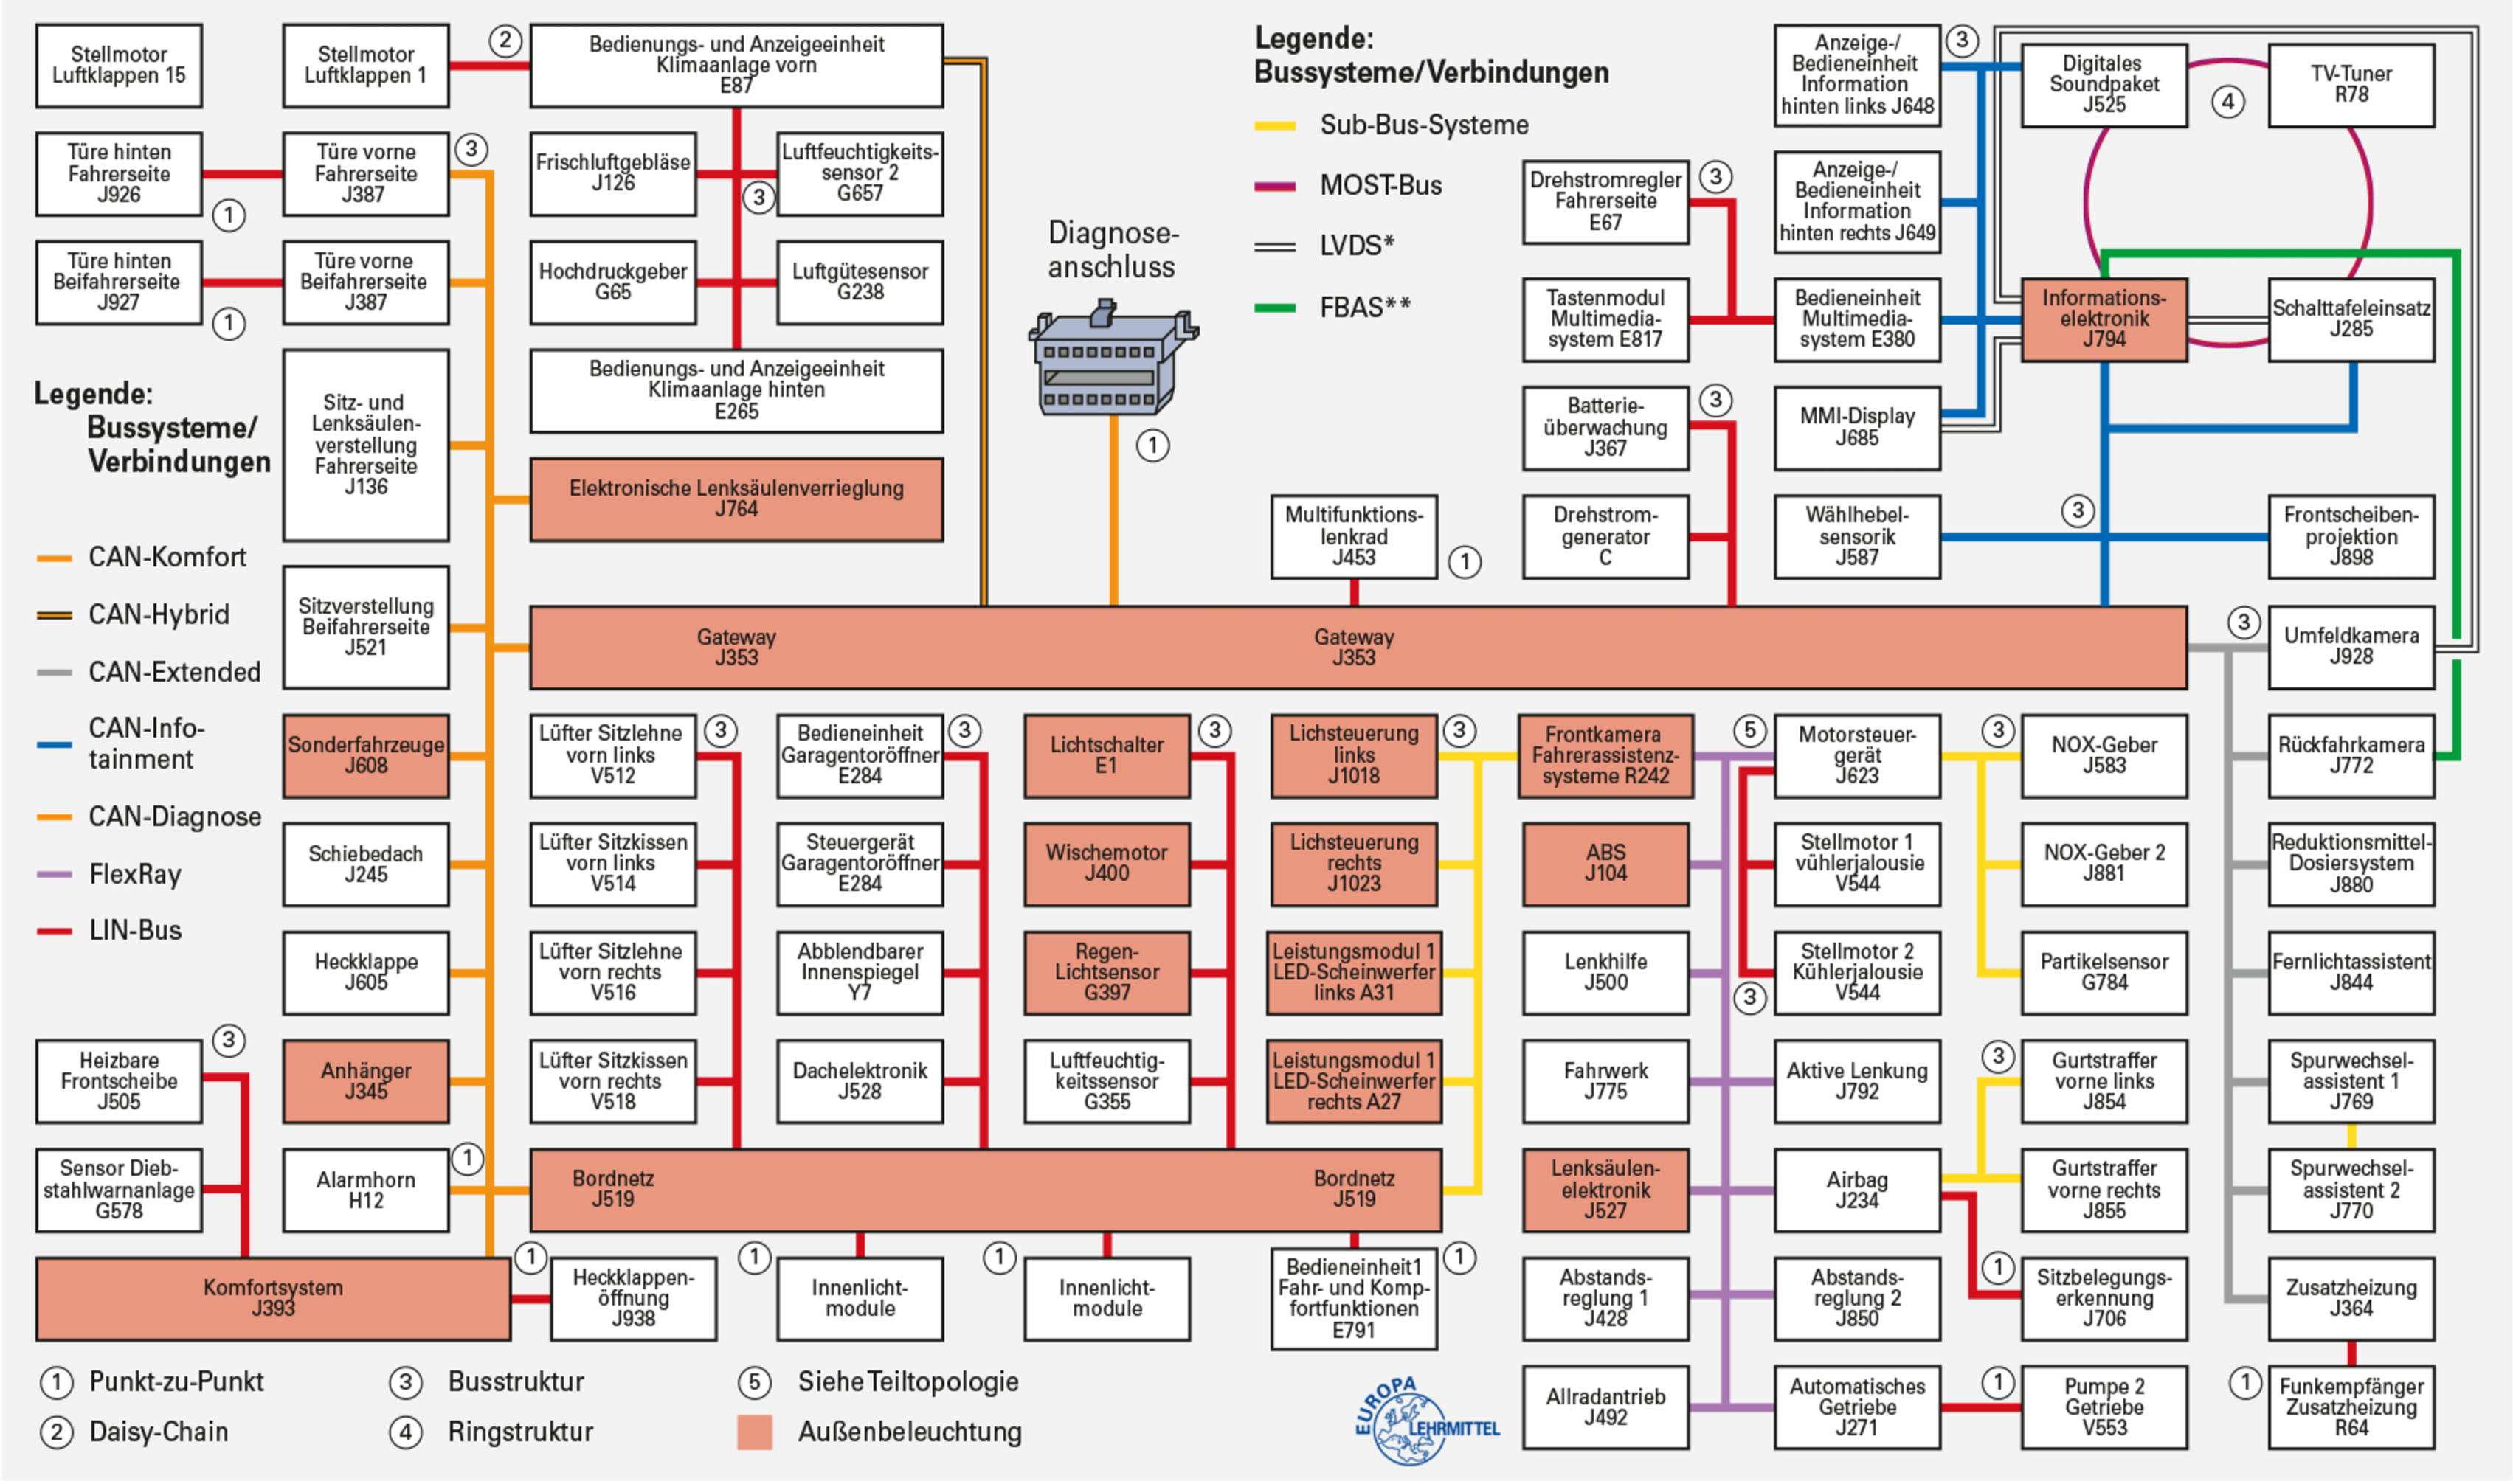
\includegraphics[width=0.9\textwidth]{images/CAN/Topologie-Datennetzwerk-Gesamtfahrzeug.png}
\caption{Topologie-Datennetzwerk-Gesamtfahrzeug, Quelle: Europa-Verlag
SimKfz}
%\label{fig:}%% anpassen
\end{figure}

\newpage

\section{CAN Klassen}\label{can-klassen}

\begin{enumerate}
\item
  \textbf{CAN Class B} (Lowspeed)

  \begin{itemize}
  \item
    bis ca. 125 kbit/s
  \item
    \textbf{Eindrahtfähig} wenn die Datenkommunikation gegeben ist, auch
    wenn eine Busleitung ausfällt
  \item
    keine Abschlusswiderstände
  \item
    \textbf{Dominant 0} low: 1 V und high: 4 V
  \item
    \textbf{Rezessiv 1} low: 5 V und high: 0 V
  \end{itemize}
\item
  \textbf{CAN Class C} (Highspeed)

  \begin{itemize}
  \item
    bis ca. 1 Mbit/s
  \item
    Nicht Eindrahtfähig
  \item
    Abschlusswiderstände $2\text{x } 60~\Omega$
  \item
    \textbf{Dominant 0} low: 1,5 V und high: 3,5 V
  \item
    \textbf{Rezessiv 1} low: 2,5 V und high: 2,5 V
  \end{itemize}
\item
  \textbf{CAN FD} (Flexible Data)

  \begin{itemize}
  \item
    bis ca. 8 Mbit/s
  \item
    Erst wenn die Daten kommen, wird die Geschwindigkeit hoch
    geschaltet.
  \end{itemize}
\end{enumerate}

\textbf{Multi-Master} Alle Steuergeräte sind gleichberechtigt. Regelung
erfolgt nach Priorität.

\textbf{Autonomes Fahren} Drive-by-Wire (alle sicherheitsrelevanten
Bauteile sind zweifach ausgelegt und zwei Bussysteme)

\newpage

\section{Aufbau CAN-Bus}\label{aufbau-can-bus}

Steuergerät sendet Nachricht auf den Datenbus.

\begin{figure}[!ht]% hier: !ht
\centering
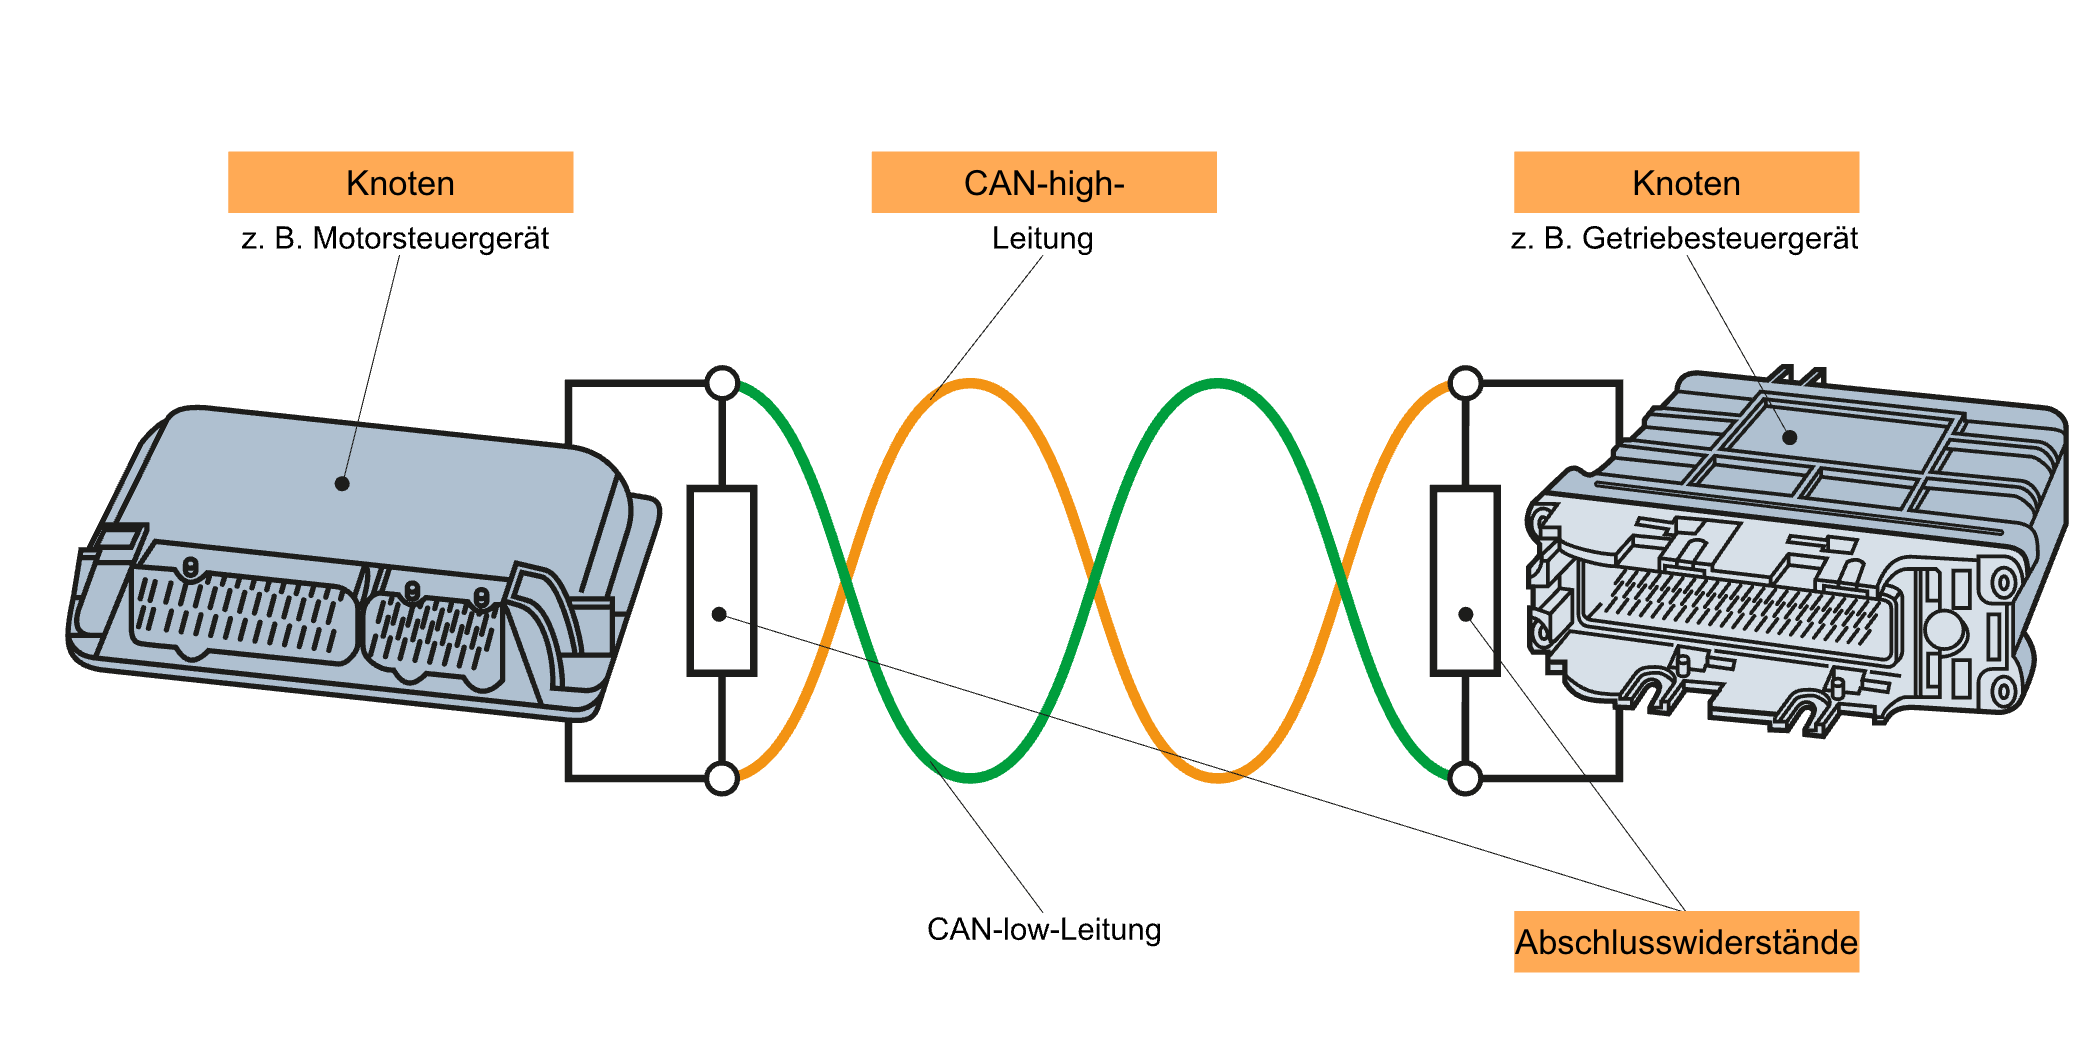
\includegraphics[width=0.6\textwidth]{images/CAN/Aufbau-CAN-Datenbus.png}
\caption{Aufbau CAN-Datenbus, Quelle: Europa-Verlag SimKfz}
%\label{fig:}%% anpassen
\end{figure}

\begin{figure}[!ht]% hier: !ht
\centering
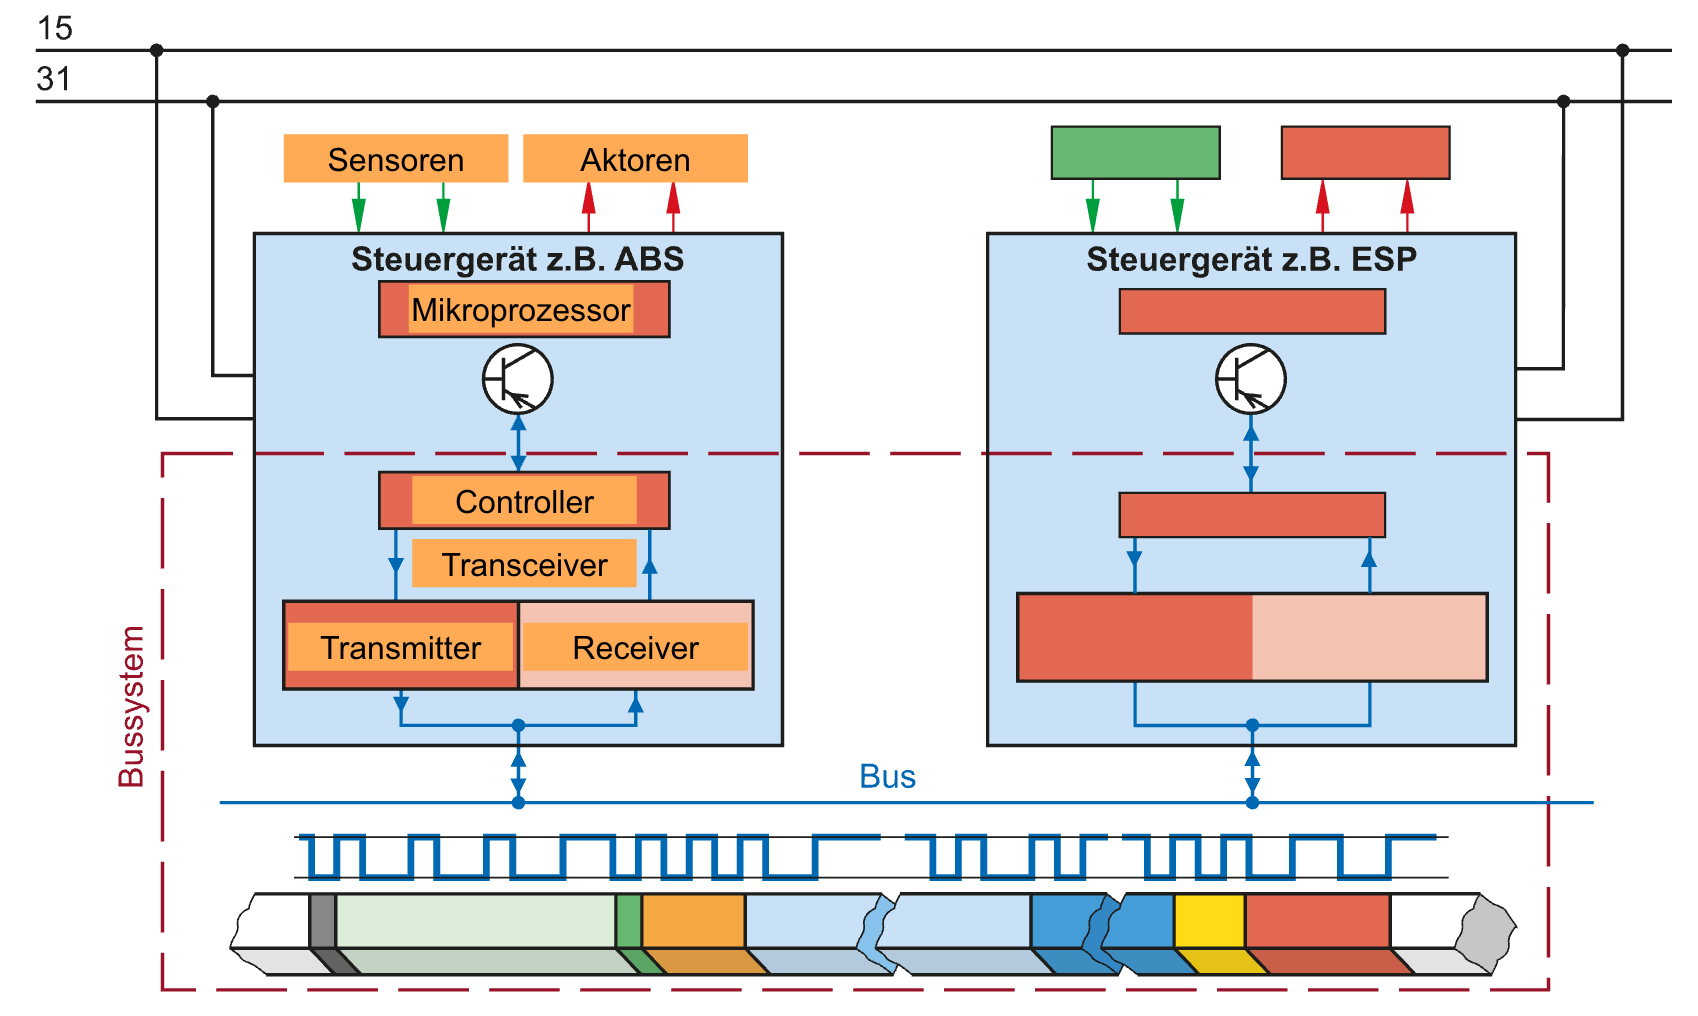
\includegraphics[width=0.6\textwidth]{images/CAN/Aufbau-elektrisches-CAN-Datenbussystem.png}
\caption{Aufbau-elektrisches-CAN-Datenbussystem, Quelle: Europa-Verlag
SimKfz}
%\label{fig:}%% anpassen
\end{figure}

\textbf{Steuergerät} (Knoten, Busteilnehmer)

\begin{enumerate}
\item
  \textbf{Microprozessor} verarbeitet die eingehenden Informationen,
  berechnet die Funktionen und steuert die Aktoren.
\item
  \textbf{Controller} filtert die für das Steuergerät notwendigen Daten
  und übermittelt sie dem Mikroprozessor.
\item
  \textbf{Transceiver} empfängt und sendet die Daten auf der Busleitung.
  Transmitter (Sender), Receiver (Empfänger)
\end{enumerate}

Beim CAN-Bussystem werden die Informationen durch Spannungsänderungen in
der Datenleitung übertragen. Dadurch empfangen alle Steuergeräte
gleichzeitig die Informationen. Die Bits werden nacheinander übertragen
(seriell).

Zwei Leitungen

\begin{enumerate}
\item
  \textbf{High-Leitung} Beim Wechsel von rezessiven (Bit = 1) zum
  dominanten (Bit = 0) Pegel steigt die Spannung.
\item
  \textbf{Low-Leitung} Beim Wechsel vom rezessiven (Bit = 1) zum
  dominanten (Bit = 0) Pegel sinkt die Spannung.
\end{enumerate}

\textbf{CAN-Buspegel}

\begin{figure}[!ht]% hier: !ht
\centering
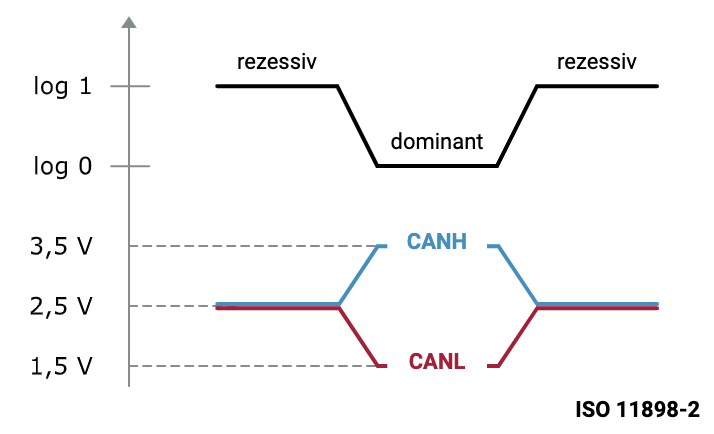
\includegraphics[width=0.4\textwidth]{images/CAN/CAN-Highspeed-Buspegel.png}
\caption[CAN-Highspeed-Buspegel, Quelle: ]{CAN-Highspeed-Buspegel,
Quelle: \footnotemark{}}
%\label{fig:}%% anpassen
\end{figure}
\footnotetext{\url{https://elearning.vector.com/mod/page/view.php?id=42}}

\begin{figure}[!ht]% hier: !ht
\centering
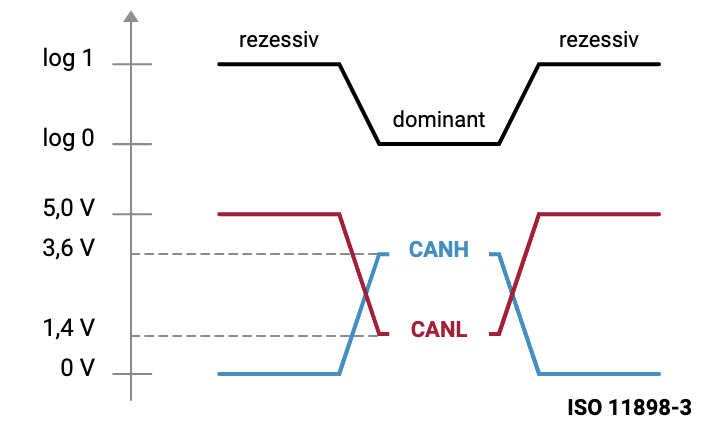
\includegraphics[width=0.4\textwidth]{images/CAN/CAN-Lowspeed-Buspegel.png}
\caption[CAN-Lowspeed-Buspegel, Quelle: ]{CAN-Lowspeed-Buspegel, Quelle:
\footnotemark{}}
%\label{fig:}%% anpassen
\end{figure}
\footnotetext{\url{https://elearning.vector.com/mod/page/view.php?id=42}}

\newpage

\section{Aufbau CAN-Nachricht -
Datenprotokoll}\label{aufbau-can-nachricht-datenprotokoll}

\begin{figure}[!ht]% hier: !ht
\centering
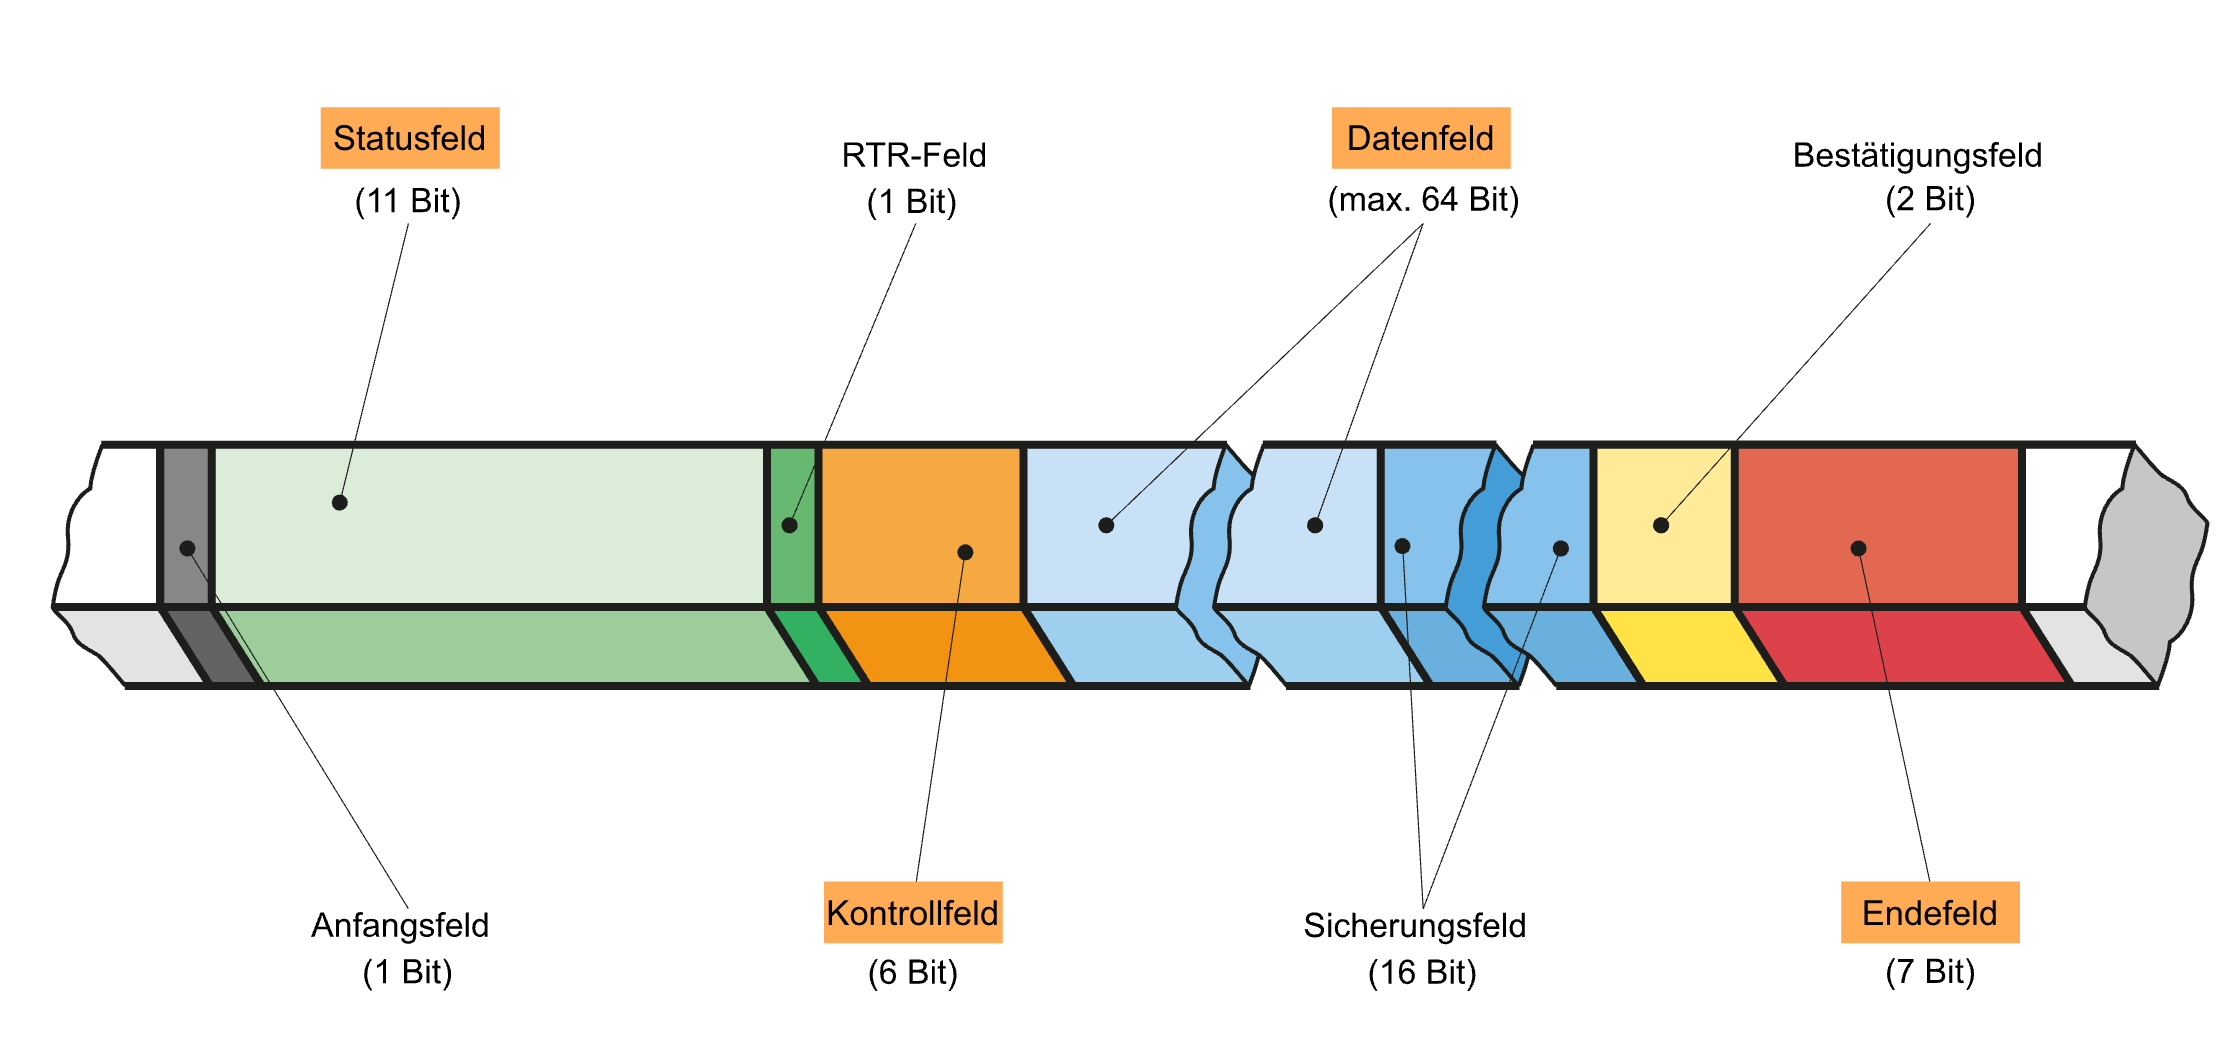
\includegraphics[width=0.6\textwidth]{images/CAN/Aufbau-CAN-Botschaft.png}
\caption{Aufbau CAN-Botschaft, Quelle: Europa-Verlag SimKfz}
%\label{fig:}%% anpassen
\end{figure}

\begin{enumerate}
\item
  Anfangsfeld (1 Bit)

  \begin{itemize}
  \item
    Beginn der Botschaft
  \end{itemize}
\item
  Statusfeld (11 Bit) Identifier

  \begin{itemize}
  \item
    Botschaftsname (Beispiel: Motordaten)
  \item
    Je niedriger die Zahl, desto wichtiger die Nachricht.
  \item
    höchste Priorität vs.~geringste Priorität
  \item
    wichtige Daten vs.~weniger wichtige Daten
  \end{itemize}
\item
  RTR (1 Bit) Remote Transmission Request Feld

  \begin{itemize}
  \item
    \textbf{0} Senden und \textbf{1} Gib mir Daten
  \end{itemize}
\item
  Kontrollfeld (6 Bit)

  \begin{itemize}
  \item
    Enthält Prüfsumme
  \end{itemize}
\item
  Datenfeld (max. 64 Bit)

  \begin{itemize}
  \item
    Motordrehzahl, Motormoment, Motortemperatur usw.
  \end{itemize}
\item
  Sicherungsfeld (16 Bit)
\item
  Bestätigungsfeld (2 Bit)
\item
  Ende (7 Bit)

  \begin{itemize}
  \item
    der Nachricht, Bus wieder frei
  \end{itemize}
\end{enumerate}

\newpage

\section{Binärzahlen umwandeln}\label{binaerzahlen-umwandeln}

\textbf{Was ist die kleinste Informationseinheit bei der
Datenübertragung?} Bit

\textbf{Wie viele Informationen können mit einem Bit übertragen werden?}
Es können zwei Informationen übertragen werden.

\lstset{language=Python}% C, TeX, Bash, Python 
\begin{lstlisting}[
	%caption={}, label={code:}%% anpassen
]
// Beispiel: 8 bit = 256 (Anzahl der Informationen)
1 Bit = 0,1 2^1 = 2
2 Bit = 00,01,10,11 2^2 = 4
3 Bit = 000,001,011,111,110,100,101,010 2^3 = 8
1 Byte = 8 bit
2^8 = 256
2^16 = 65536 
\end{lstlisting}

\textbf{Zweier Potenzen}

$2^0 = 1 \\ 2^1 = 2 \\2^2 = 4 \\2^3 = 8 \\2^4 = 16 \\2^5 = 32 \\2^6 = 64 \\2^7 = 128 \\2^8 = 256$

\textbf{Binär in Dezimal}

\lstset{language=Python}% C, TeX, Bash, Python 
\begin{lstlisting}[
	%caption={}, label={code:}%% anpassen
]
 1 0 1 1 1 // Binärzahl (5-stellig)
16 8 4 2 1 // 2-Potenz
16 0 4 2 1 // Addieren
__________
Dezimal: 23
\end{lstlisting}

\textbf{Dezimal in Binär}

\lstset{language=Python}% C, TeX, Bash, Python 
\begin{lstlisting}[
	%caption={}, label={code:}%% anpassen
]
Dezimal: 99
Test 99 < 128        // also 7-stellige Binärzahl
64 32 16  8  4  2  1 // 2-Potenz
64+32                // Addieren
96             +2 +1 
 1  1  0  0  0  1  1 // Binärzahl 
\end{lstlisting}

\newpage

\section{Fehler am CAN-Bus}\label{fehler-am-can-bus}

Messung am OBD-Stecker direkt machen.

\textbf{Messpunkte} CAN-High (Pin6) und CAN-Low (Pin14)

\textbf{Gutbild} (CAN-Low-Signal \& CAN-High-Signal sind
spiegelverkehrt)

\begin{figure}[!ht]% hier: !ht
\centering
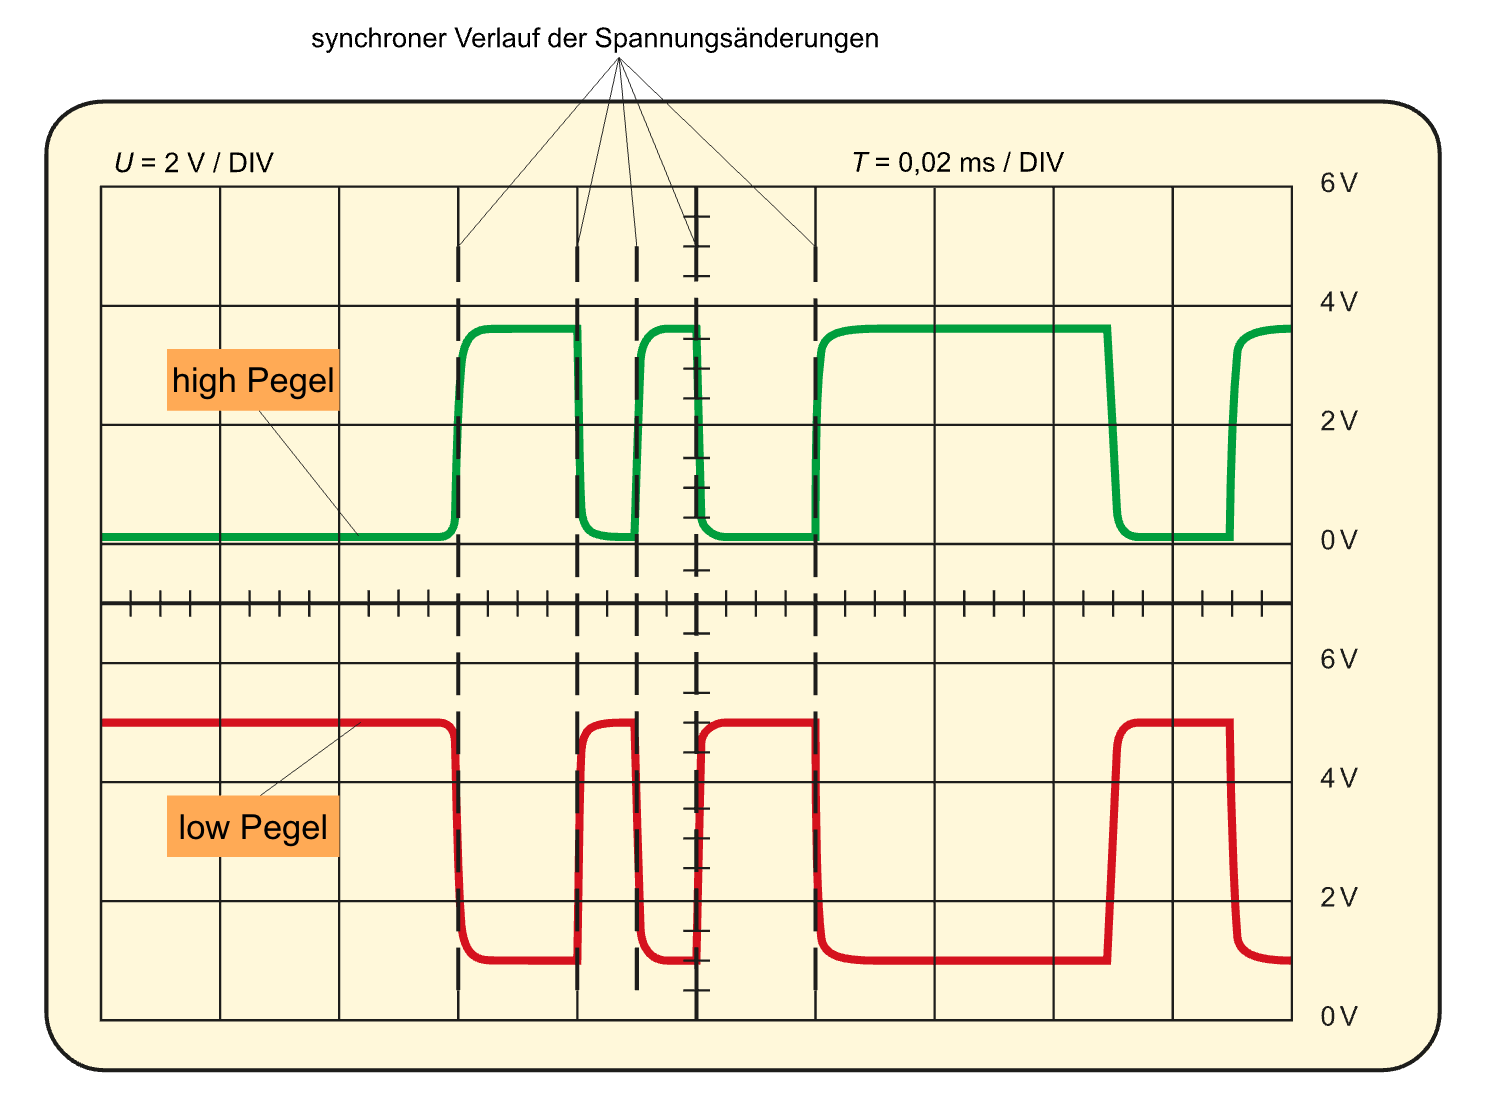
\includegraphics[width=0.4\textwidth]{images/CAN/Fehlerfreies-Signal-CAN-Bus.png}
\caption{Fehlerfreies Signal CAN-Bus, Quelle: Europa-Verlag SimKfz}
%\label{fig:}%% anpassen
\end{figure}

\begin{figure}[!ht]% hier: !ht
\centering
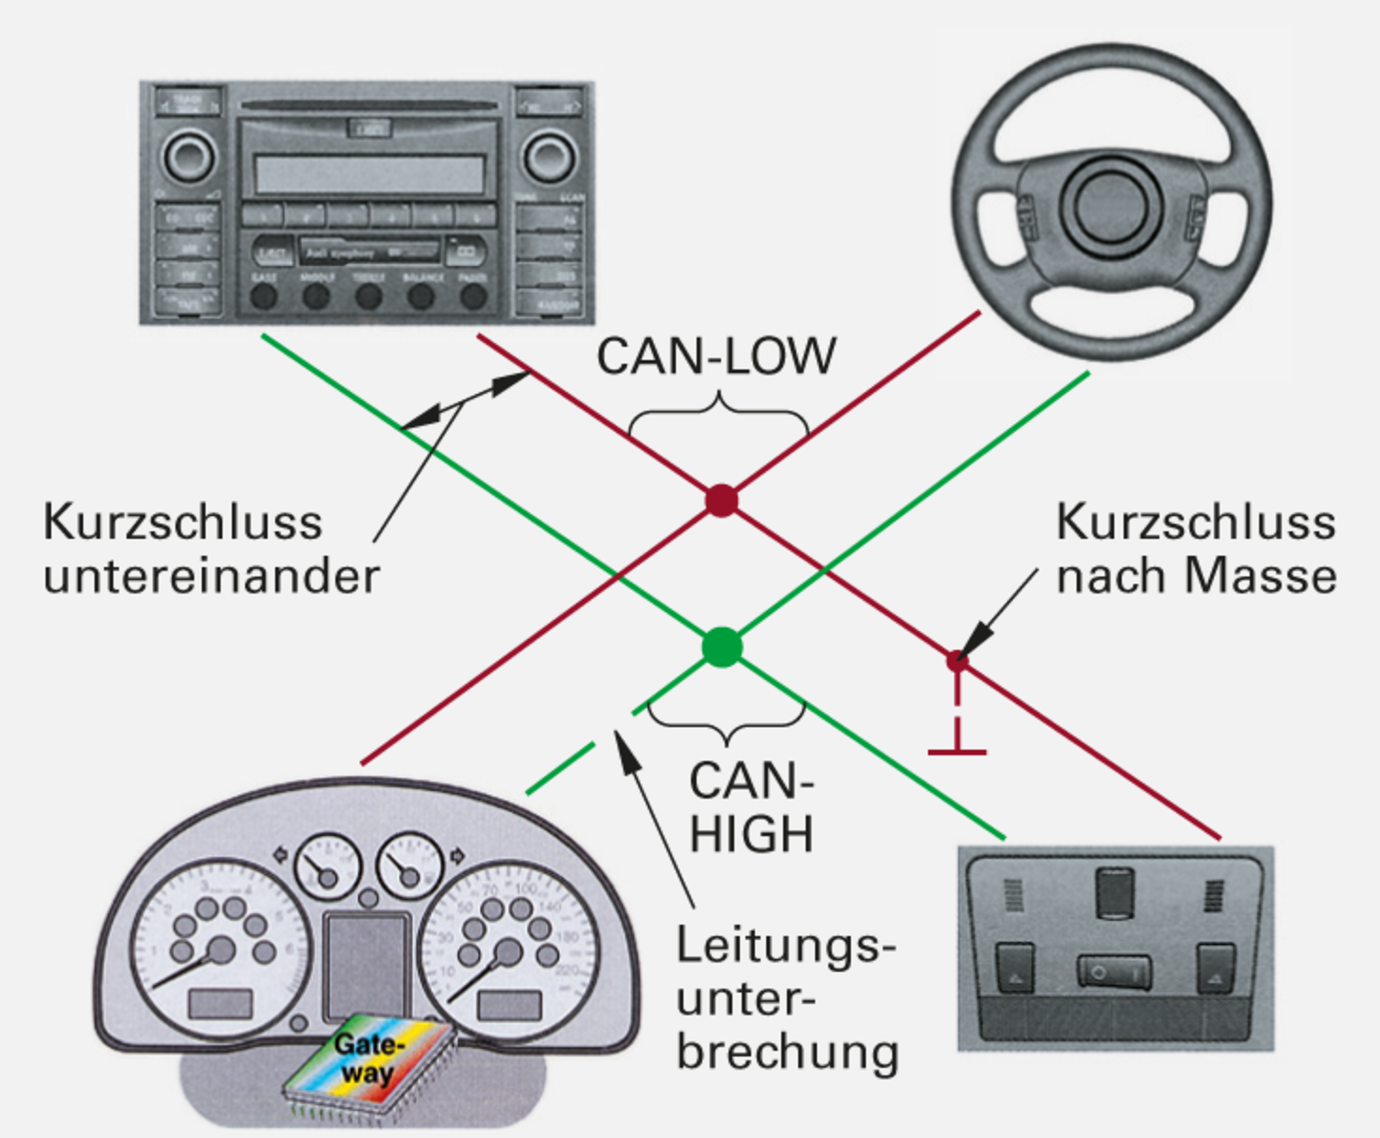
\includegraphics[width=0.4\textwidth]{images/CAN/Fehlermoeglichkeiten-CAN-Bus.png}
\caption{Fehlermöglichkeiten CAN-Bus, Quelle: Europa-Verlag SimKfz}
%\label{fig:}%% anpassen
\end{figure}

\begin{figure}[!ht]% hier: !ht
\centering
\includegraphics[width=0.8\textwidth]{images/CAN/Fehler-CAN-Bus.png}
\caption{Fehler CAN-Bus, Quelle: Europa-Verlag Arbeitsblätter
Kfz-Technik Lernfeld 9-14}
%\label{fig:}%% anpassen
\end{figure}

\newpage

\subsection{Keine Kommunikation zum SG
möglich}\label{keine-kommunikation-zum-sg-moeglich}

\begin{enumerate}
\item
  CAN-High überprüfen

  \begin{itemize}
  \item
    \textbf{Messpunkt:} Oszi an (Pin6 \& Masse)
  \end{itemize}
\item
  CAN-Low überprüfen

  \begin{itemize}
  \item
    \textbf{Messpunkt:} Oszi an (Pin14 \& Masse)
  \end{itemize}
\end{enumerate}

\textbf{kein Spannungsverlauf?}

\begin{itemize}
\item
  Beide Leitungen durchmessen
\item
  CAN-High (SG gegen Masse)
\item
  CAN-Low (SG gegen Masse)
\end{itemize}


%\chapter{Elektromotoren}
%\chapter{Bordnetz}
%\chapter{Beleuchtung}

\chapter{Formelsammlung -- Elektrik}
%ju 17-Sep-22 FS-Elektrik.tex
\section{Grundlagen}\label{grundlagen}

\textbf{Eingabe Rechner}

\begin{enumerate}
\def\labelenumi{\alph{enumi}.}
\setcounter{enumi}{25}
\item
  B. $20~mV = \num{20,0e-3} \curvearrowright$ Rechner:
  $20\text{EE}-3 = 0,02$
\end{enumerate}

$10^3 = 1.000 = \num{1,0e3}$

$10^{-3} = \frac{1}{1000} = 0,001 = \num{1,0e-3}$

$10^6 = 1.000.000 = \num{1,0e6}$

$10^{-6} = \frac{1}{1.000.000} = 0,000.001 = \num{1,0e6}$

\textbf{Größen}

$\boxed{K = \num{1,0e3} \quad M = \num{1,0e6} \quad G = \num{1,0e9} \quad T = \num{1,0e12}}$

$\boxed{m = \num{1,0e-3} \quad \mu = \num{1,0e-6} \quad n = \num{1,0e-9} \quad p = \num{1,0e-12}}$

\textbf{Einheiten}

\textbf{Faktor} Länge 10, Fläche 100, Volumen 1000

$\boxed{\mu m \quad mm \quad cm \quad dm \quad m \quad km}$

$1~l = 1~dm^3 \quad 10~ml = 1~cl = 0,01~l$

$\frac{g}{cm^3} \quad \frac{kg}{dm^3} \quad \frac{t}{m^3}$

\textbf{Prozent} $10~\% = \frac{10}{100} = 0,1$

\textbf{km/h in m/s}
$\Rightarrow \frac{km/h}{3,6} \quad \frac{km}{h} \Rightarrow \frac{m}{s} \Rightarrow \frac{1000}{3600}$

\textbf{Stunden:Min:Sek in Dezimalstunden}
$\Rightarrow \text{h} + \frac{Min}{60} + \frac{Sek}{60 \cdot 60}$

\textbf{Zoll in mm} $1~\text{Zoll} = 25,4~mm$

\textbf{Kreisfläche}
$\boxed{\frac{d^2 \cdot \pi}{4}} \quad \text{Hinweis: }\frac{\pi}{4} \approx 0,785$

\textbf{Masse} $\boxed{m = V \cdot \rho}$ Dichte bleibt immer gleich
$\to$ Volumen ändert sich

\textbf{Volumen} $\boxed{V = A \cdot h}$

\textbf{Umfang} $\boxed{Umfang = d \cdot \pi}$

\textbf{Drehmoment} $\boxed{M = F \cdot r}$

\section{Fach Elektrotechnik}\label{fach-elektrotechnik}

\textbf{SPANNUNG} $U~\text{Volt}~[V]$

\textbf{STROM} $I~\text{Ampere}~[A]$

\textbf{WIDERSTAND} $R~\text{Ohm}~[\Omega]$

\textbf{Reihe}

\begin{enumerate}
\item
  Strombegrenzung
\item
  Spannungsteilung
\end{enumerate}

\textbf{Parallel}

\begin{enumerate}
\item
  Stromflusserhöhung
\item
  Leistungsteilung $\boxed{R_{ges} = \frac{R_{Teil}}{n}}$
\end{enumerate}

\textbf{OHMSCHE GESETZ}

$\boxed{I = \frac{U}{R}} \quad \bigl[\frac{V}{\Omega}\bigl] = A \quad  \boxed{R = \frac{U}{I}} \quad \bigl[\frac{V}{A}\bigl] = \Omega \quad  \boxed{U = R \cdot I} \quad [\Omega \cdot A] = V$

\textbf{STROMDICHTE}

$\boxed{J = \frac{I}{A}} \quad \bigl[\frac{A}{mm^2}\bigl] \quad  \boxed{I = J \cdot A} \quad \bigl[\frac{A \cdot mm^2}{mm^2}\bigl] = A \quad  \boxed{A = \frac{I}{J}} \quad \bigl[\frac{A \cdot mm^2}{A}\bigl] = mm^2$

\textbf{LEITWERT} $S$ Siemens

$\boxed{G = \frac{1}{R}} \quad \bigl[\frac{1}{\Omega}\bigl] = S \quad \boxed{R = \frac{1}{G}} \quad \bigl[\frac{1}{S} = \Omega\bigl]$

\textbf{LEITERWIDERSTAND}

$\boxed{R_l = \frac{\rho \cdot l}{A}} \quad \bigl[\frac{\Omega \cdot mm^2 \cdot m}{m \cdot mm^2}\bigl] = \Omega \quad \boxed{A = \frac{\rho \cdot l}{R_l}} \quad \bigl[\frac{\Omega \cdot mm^2 \cdot m}{m \cdot \Omega}\bigl] = mm^2$

$\boxed{l = \frac{R_l \cdot A}{\rho}} \quad \bigl[\frac{\Omega \cdot mm^2 \cdot m}{\Omega \cdot mm^2}\bigl] = m$

\textbf{SPEZIFISCHER WIDERSTAND} $\rho$ rho

$\rho \quad \bigl[\frac{\Omega \cdot mm^2}{m}\bigl] \quad \rho_{Cu} = 0,0178~\frac{\Omega \cdot mm^2}{m}$

\textbf{ELEKTRISCHE LEITFÄHIGKEIT} $\kappa$ Kappa

$\boxed{\kappa = \frac{1}{\rho}} \quad \bigl[\frac{m}{\Omega \cdot mm^2}\bigl] \quad \kappa_{Cu} = 56~\frac{m}{\Omega \cdot mm^2}$

\textbf{REIHENSCHALTUNG}

$\boxed{U_{ges} = U_{R_1} + U_{R_2} + U_{R_3} + \dots + U_{R_n}} \quad \bigl[V + V + V\bigl] = V$

$\boxed{U_{teil} = \frac{U_{ges}}{n}} \quad \bigl[\frac{V}{1}\bigl] = V$

$\boxed{I_{ges} = I_{R_1} = I_{R_2} = I_{R_3} = \dots = I_{R_n}} \quad \bigl[A = A = A\bigl] = A$

$\boxed{R_{ges} = R_1 + R_2 + R_3 + \dots + R_n} \quad \bigl[\Omega + \Omega + \Omega\bigl] = \Omega$

\textbf{SPANNUNGSVERLUST} (Spannungsfall)

$U_{ges} = U_v + U_k;\quad U_k = U_{ges} - U_v;\quad U_v = U_{ges} - U_k$

$U_v = R_l \cdot I;\quad R_l = \frac{\rho \cdot l}{A} \quad \bigl[\frac{\Omega \cdot mm^2 \cdot m}{m \cdot mm^2}\bigl] = \Omega$

$U_k = U_{ges} - R_l \cdot I$

$\boxed{U_v = \frac{\rho \cdot l \cdot I}{A}} \quad \bigl[\frac{\Omega \cdot mm^2 \cdot m \cdot A}{m \cdot mm^2}\bigl] = V \quad \rho_{Cu} = 0,0178~\frac{\Omega \cdot mm^2}{m}$

$U_{v_{~\%}} = \frac{U_v \cdot 100}{U_{ges}} \quad \bigl[\frac{V \cdot ~\%}{V}\bigl] = ~\%$

$\boxed{U_{v_{max}} = 0,5~V}$

$\boxed{\text{max. Leiterwiderstand} = 1~\Omega}$ (außer
Starterhauptleitung)

\textbf{INNENWIDERSTAND} (von Spannungsquellen)

$U_q = U_k + U_i \quad [V + V] = V$

$U_k = U_q - U_i \quad [V - V] = V$

$U_i = U_q - U_k \quad [V - V] = V$

$U_i = I \cdot R_i \quad [A \cdot \Omega] = V$

$U_k = I \cdot R_a \quad [A \cdot \Omega] = V$

$I = \frac{U_i}{R_i} \quad [\frac{V}{\Omega}] = A$

$I = \frac{U_k}{R_a} \quad [\frac{V}{\Omega}] = A$

$I = \frac{U_q}{R_{ges}} \quad [\frac{V}{\Omega}] = A$

$I = \frac{U_q}{R_i + R_a} \quad [\frac{V}{\Omega + \Omega}] = A$

$\boxed{U_k = U_q - I \cdot R_i} \quad [V - A \cdot \Omega \to V - V] = V$

$\boxed{R_i = \frac{U_i}{I}} \quad [\frac{V}{A}] = \Omega$

$\boxed{U_k = U_q - U_i - U_v} \quad \boxed{R_{ges} = R_i + R_l + R_\text{ü} + R_{La}}$

\emph{Herleitung}

$U_k = U_q - I \cdot R_i$ $\quad | +I \cdot R_i$

$U_k + I \cdot R_i = U_q - I \cdot R_i + I \cdot R_i$ $\quad | -U_k$

$-U_k + U_k + I \cdot R_i = U_q - U_k$ $\quad | :I$

$\frac{I \cdot R_i}{I} = \frac{U_q - U_k}{I}$
$\quad \bigl[\frac{V - V}{A} \to \frac{V}{A}\bigl] = \Omega$

$R_i = \frac{U_i}{I}$

\textbf{PARALLELSCHALTUNG}

$\boxed{I_{ges} = I_{R_1} + I_{R_2} + I_{R_3} + \dots + I_{R_n}}\quad [A + A + A] = A$

$\boxed{U_{ges} = U_{R_1} = U_{R_2} = U_{R_3} = \dots = U_{R_n}}\quad [V = V = V] = V$

$\boxed{R_{ges} = \frac{1}{\frac{1}{R_1} + \frac{1}{R_2} + \frac{1}{R_3} + \dots + \frac{1}{R_n}}} \quad \bigl[\frac{1}{\frac{1}{\Omega} + \frac{1}{\Omega} + \frac{1}{\Omega}} = \frac{1}{\frac{1}{\Omega}} = \frac{1}{S}\bigl] = \Omega$

Ersatzwiderstand
$\boxed{R_{ges} = \frac{R_{Teil}}{n}} \quad \bigl[\frac{\Omega}{1}\bigl] = \Omega \quad \to \text{Anzahl } n = \frac{R_{Teil}}{R_{ges}} \quad \bigl[\frac{\Omega}{\Omega}\bigl] = 1$

n = Anzahl der Widerstände (gleich große Widerstände)

$\boxed{R_{ges} = \frac{R_1 \cdot R_2}{R_1 + R_2}}$

$R_{ges} = \frac{1}{\frac{1}{R_1} + \frac{1}{R_2} + \frac{1}{R_3}}$

$\to R_{1} = \frac{1}{\frac{1}{R_{ges}} - \frac{1}{R_2} - \frac{1}{R_3}} \quad \to R_{2} = \frac{1}{\frac{1}{R_{ges}} - \frac{1}{R_1} - \frac{1}{R_3}} \quad \to R_{3} = \frac{1}{\frac{1}{R_{ges}} - \frac{1}{R_1} - \frac{1}{R_2}}$

\textbf{LEISTUNG} $P$ (Power) Watt, $[W], [kW]$

$\boxed{P = U \cdot I} \quad [V \cdot A] = W$

$\boxed{U = \frac{P}{I}} \quad [\frac{W}{A} \to \frac{V \cdot A}{A}] = V$

$\boxed{I = \frac{P}{U}} \quad [\frac{W}{V} \to \frac{V \cdot A}{V}] = A$

\textbf{wenn $I$ fehlt} (Einsetzverfahren)

$P = U \cdot I \quad [V \cdot A] = W, \quad I = \frac{U}{R} \quad [\frac{V}{\Omega}] = A$

$P = U \cdot \frac{U}{R} \to \boxed{P = \frac{U^2}{R}} \quad [\frac{V \cdot V}{\Omega} \to A \cdot V] = W$

\textbf{wenn $U$ fehlt} (Einsetzverfahren)

$P = U \cdot I \quad [V \cdot A] = W, \quad U = R \cdot I \quad [\Omega \cdot A] = V$

$P = R \cdot I \cdot I \to \boxed{P = R \cdot I^2} \quad [\Omega \cdot A \cdot A \to V \cdot A] = W$

\textbf{Lampe} $12~V/55~W$

\begin{enumerate}
\item
  $R_{La} = \frac{U^2}{P}$
\item
  $I_{tat} = \frac{U_k}{R_{La}} = \frac{U_{ges} - U_v}{R_{La}}$
\item
  $P_{tat} = U_k \cdot I_{tat}$
\end{enumerate}


\chapter{Übungen}
\section{Ü01 Fragen zum Schaltplan Audi-A3 - Lösung}
%ju 31-Dez-22 U01-Schaltplan-AudiA3-Loesung.tex
\textbf{1. Beschreiben Sie die Spannungsversorgung für die Pumpe für
Kühler der Abgasrückführung.}

\begin{enumerate}
\item
  Stromverteiler (87)
\item
  über Sicherung (24)
\item
  Steckverbindung ($T_{40/11}$)
\item
  Plusverbindung $B_{321}$
\item
  Pumpe für Kühler der Abgasrückführung $V_{400}$ (Pin 2)
\item
  Steckverbindung ($T_{14/9}$)
\item
  Masseverbindung (394)
\item
  Massepunkt (655) am Scheinwerfer links
\end{enumerate}

\textbf{2. Welche Fehler können auftreten und welche Auswirkungen haben
diese?}

\textbf{Welches Signal erwarten wir?} PWM-Signal

\begin{enumerate}
\item
  Bauteil defekt
\item
  Sicherung defekt
\item
  Leitungsunterbrechung (Signalleitung, Plusleitung, Masseleitung)
\item
  Übergangswiderstand (Spannungsfall im Stecker oder Leitungen)
\item
  Masseschluss oder Plusschluss
\end{enumerate}

\textbf{Mögliche Fehler}

\begin{enumerate}
\item
  MIL-Lampe an $\to$ Abgas relevanter Fehler (Steuerhinterziehung)
\item
  AGR-Ventil klemmt fest, wenn offen $\to$ Leistungsverlust im warmen
  Zustand
\end{enumerate}

\textbf{3. Fehler Abgastemperaturgeber 1, 3, 4 sind im Fehlerspeicher
abgelegt. Nennen Sie mögliche Fehlerursachen.}

\begin{enumerate}
\item
  Bauteil defekt (Temperatursensoren)
\item
  plusseitig
\end{enumerate}

\textbf{4. Motordrehzahlgeber hat kein Signal. Welche möglichen Ursachen
liegen vor?}

\textbf{Was erwarten wir?} Hallgeber, Versorgungsspannung (5 V)

\begin{enumerate}
\item
  Masseverbindung
\item
  Bauteil defekt
\item
  Plusverbindung (5 V)
\end{enumerate}

\textbf{5. Ihnen liegt ein Fehler zur Kraftstoffvorratsanzeige vor.
Nennen Sie mögliche Fehler.}

\begin{enumerate}
\item
  Geber defekt
\item
  Gebermasse
\item
  Übergangswiderstand
\item
  Leitungsunterbrechung von (Pin 3 + 4) zum Kombiinstrument
\item
  Widerstand defekt
\end{enumerate}

\section{Ü02 Motor startet nicht. Welche Fragen stellen Sie den Kunden? - Lösung}
%ju 17-Sep-22 U02-Motor-startet-nicht-Loesung.tex
\textbf{Fragen an den Kunden}

\begin{enumerate}
\item
  Dreht der Motor?
\item
  Seit wann ist der Fehler?
\item
  Ist der Motor zwischendurch angesprungen? (sporadischer Fehler)
\item
  Fängt die Beleuchtung an zu flackern?
\item
  Stand das Fahrzeug länger?
\item
  Brauchte der Motor lange, um zu starten?
\item
  Wurde Starthilfe gegeben?
\end{enumerate}

\textbf{Prüfung am Fahrzeug}

\begin{enumerate}
\item
  Batterie prüfen (Quellenspannung messen)
\item
  Anlasser macht keine Geräusche beim Versuch den Motor zu starten
\item
  Spannungsversorgung am Anlasser prüfen (Sicherung / Relais
  ausschließen)
\item
  Masseversorgung prüfen: Widerstandsmessung, Spannungsfallmessung
\end{enumerate}

\textbf{Diagnose}

Das Masseband ist durch einen Übergangswiderstand defekt.

\textbf{Erklärung an den Kunden}

Das Masseband klaut dem Anlasser die Spannung.

\textbf{Erklärung an den Lehrling}

Das Masseband vom Motor ist durch einen Übergangswiderstand beschädigt,
damit haben wir eine geringe Leitfähigkeit und dadurch einen geringen
Stromfluss.

\section{Ü03 Prüfungshinweise - Automatikgetriebe}
%ju 13-Aug-22 U03-Pruefungshinweise-Automatikgetriebe.tex
\textbf{1) Dialogannahme -- Fragen an den Kunden, die das Problem
eingrenzen.}

\begin{enumerate}
\item
  Welche Fehlermeldung?
\item
  Wann und wo tritt der Fehler auf? (Betriebszustand: Drehzahl,
  Geschwindigkeit, Temperatur?)
\item
  Problem reproduzierbar?
\end{enumerate}

\textbf{2) Prüfvoraussetzung}

\begin{enumerate}
\item
  Batteriespannung prüfen
\item
  Spannungsversorgung am SG (Sicherung)
\item
  Ölstand Getriebe (Prüftemperatur)
\item
  Stecker vom Getriebe $\to$ Kontrolle auf Feuchtigkeit und Korrosion
\end{enumerate}

\textbf{3) Welche Sicherung prüfen Sie zuerst?}

vgl. Schaltplan

\textbf{4) Funktionsprüfung Magnetventil}

\begin{enumerate}
\item
  Stellgliedtest
\item
  Oszilloskop
\item
  Widerstand messen von Spule
\end{enumerate}

\textbf{Am Ende $\dots$ Getriebesteuergerät defekt.}



\chapter{Diagnose}
%ju 31-Dez-22 Diagnose.tex
\textbf{Fehlersuche in einem immer stärker vernetzten Fahrzeugsystem}
(\textcite{respondeck:2019:servicetechniker}).

\begin{enumerate}
\item
  \textbf{Fahrzeugannahme}

  \begin{itemize}
  \item
    Das Fahrzeug sollte im Beisein des Kunden einer \emph{Sicht- und
    Funktionsprüfung} unterzogen werden und den Kunden zu dem Fehler
    befragen.
  \item
    kurzen >>Rundum-Check<< des Fahrzeugs, um weitere
    (sicherheitsrelevante) Mängel aufdecken. In diesem Zusammenhang
    können auch Vorschäden dokumentiert und dem Kunden gezeigt werden,
    um etwaigen Ansprüchen nach Rückgabe des Fahrzeugs entgegenzuwirken.
    Ein Foto von allen Seiten hilft im Streitfall bei der Klärung.
  \item
    Bei \textbf{sporadischen Fehlern} zu hinterfragen, unter welchen
    Umständen und bei welchen Bedingungen der Fehler aufgetreten ist, um
    ihn zu reproduzieren, zu können.

    \begin{itemize}
    \item
      Betriebszustand und Fahrsituation (Motor kalt/warm; Last;
      Drehzahl; Fahrgeschwindigkeit; Beschleunigen/Verzögern;
      Rechts-/Linkskurve usw.)
    \item
      Einsatzbedingungen (hohe/geringe Außentemperatur; Witterung
      Beispiel: Nässe, Regen)
    \item
      Schaltzustände von Teilsystemen (Licht an/aus; Klimaanlage,
      Sitzheizung etc. an/aus)
    \item
      Besonderheiten (Anhängerbetrieb; Zubehör im Innenraum $\to$
      elektromagnetische Störungen/Störung des Bordnetzes durch
      angeschlossene Geräte
    \item
      Technische Änderungen (Motoreingriffe; Umbereifung;
      Fahrwerksänderungen)
    \item
      Kürzlich von einer anderen Werkstatt durchgeführte Reparaturen
    \end{itemize}
  \item
    korrekten \textbf{Fahrzeugschlüssel} vom Kunden übernehmen. (sog.
    Benutzer-Adaption)

    \begin{itemize}
    \item
      Sitz und Spiegeleinstellung, Radiosender und -lautstärke
    \item
      Aktivierung/Deaktivierung von Assistenzsystemen
      (Fahrlichtsteuerung, Regen-/Lichtsensor, Einparkassistent,
      Spurhalteassistent)
    \item
      Tippblinken
    \item
      Automatisches Verriegeln während der Fahrt, automatisches
      Wiederverschließen
    \item
      Ansprechverhalten des Fahrpedals
    \item
      Schaltzeitpunkt des automatischen Getriebes
    \end{itemize}
  \end{itemize}
\item
  \textbf{Fehlerspeicher auslesen}

  \begin{itemize}
  \item
    bei >>Mehreren Kundenbeanstandungen<< im ersten Schritt sollte bei
    der Bewertung der Fehler eine gemeinsame Ursache in Betracht gezogen
    und erst, wenn diese auszuschließen ist, jeder Fehler für sich
    betrachtet werden.
  \item
    gesamten Fehlerspeicher des Fahrzeugs auslesen und bei mehreren
    Fehlern zunächst eine gemeinsame Ursache zu suchen.
  \item
    Vor dem Löschen eines Fehlerspeichers dokumentieren
  \item
    \textbf{Klassische Fehler} vs.~\textbf{Plausibilitätsfehler}
  \end{itemize}
\item
  \textbf{Messwerte/Istwerte/Parameter auslesen}

  \begin{itemize}
  \item
    Prüfen, ob die vom SG mithilfe der Sensorik erfassten Daten der
    Realität entsprechen.
  \item
    Im Zweifel sollten die Werte mithilfe eines separaten Messgerätes
    ermittelt und abgeglichen werden.
  \end{itemize}
\item
  \textbf{Stellgliedtest bei Fehlern im Bereich der Aktorik}

  \begin{itemize}
  \item
    Bauteil mithilfe des Diagnosegeräts ansteuern oder anhand von
    Messwerten überprüfen, ob es reagiert. Prüfen, ob das gewünschte
    Ergebnis tatsächlich erzielt wird.
  \item
    Der Stellgliedtest sollte über das Diagnosegerät durchgeführt
    werden. Eine Überprüfung durch >>Provozieren<< einer Ansteuerung ist
    nicht aussagekräftig, da oftmals nicht alle Bedingungen für das
    Ansteuern des jeweiligen Aktors bekannt sind. Selbst der Vergleich
    mit einem anderen Fahrzeug (gleiches Modell, gleicher Motor,
    gleiches Baujahr) scheitert, wenn sich der Stand der Software der SG
    unterscheidet.
  \end{itemize}
\item
  \textbf{Messungen mit Multimeter und Oszilloskop}

  \begin{itemize}
  \item
    sollte es Hinweise auf fehlerhafte Sensoren, Aktoren oder Systeme
    geben. Ursache des Fehlers ermitteln.
  \item
    Die Größen Spannung, Strom und Widerstand müssen mithilfe der
    Prüfanleitung des Herstellers gemessen werden.
  \end{itemize}
\end{enumerate}

\textbf{Sporadischer Fehler} also wiederkehrend, aber nicht permanent
vorhanden

\textbf{Klassische Fehler} sind solche, bei denen das SG ein Problem des
jeweiligen Bauteils messtechnisch ermittelt und den Fehler (Beispiel:
>>Signalspannung zu hoch<<) als solchen im SG hinterlegt hat. Beim
Auftreten solcher Fehler kann man sofort mit der Fehlersuche im Rahmen
von Messungen im Bereich des jeweiligen Bauteils beginnen.

\textbf{Plausibilitätsfehler} legt das SG dagegen im Fehlerspeicher ab,
wenn die ankommenden Informationen unplausibel sind, also nicht
zueinanderpassen oder Sprünge enthalten, die ohne weitere Informationen
nicht zu erklären sind. Beim Auftreten von Plausibilitätsfehlern sollte
man klären, welche unpassenden Informationen zu dem Fehler geführt
haben.

\textbf{Beispiel 1) Fehler: Heißfilmluftmassenmesser (Diesel) >>Signal
unplausibel<<}

Der Heißfilmluftmassenmesser hat beim Diesel hauptsächlich die Aufgabe,
die Volllastmenge zu begrenzen und die Abgasrückführrate zu ermitteln.

Die AGR-Rate wird bestimmt, indem das SG die Soll-Luftmasse im aktuellen
Betriebszustand aus Hubraum, Drehzahl, Ladedruck usw. ermittelt, und die
vom Luftmassenmesser ermittelte Ist-Luftmasse hiervon abzieht. Bei einer
AGR-Rate von $10~\%$ sollte die vom Luftmassenmesser ermittelte
Luftmasse also $10~\%$ geringer sein, als die theoretisch unter den
aktuellen Bedingungen angesaugte Luftmasse. Wäre nun beispielsweise die
Abgasrückführung verrußt, so reduziert sich die rückgeführte Abgasmenge
bei gleicher Stellung des AGR-Ventils. Der Rückgang der vom
Heißfilmluftmassenmesser ermittelten Luftmasse läge dann unter $10~\%$
und das SG meldet, dass das >>Signal unplausibel<< ist.

\textbf{Beispiel 2) Fehler: Heißfilmluftmassenmesser (Diesel) >>Signal
unplausibel<<}

Der gleiche Fehler des Heißfilmluftmassenmessers kann auftreten, wenn
der Luftfilter erneuert wird, ohne dies dem SG durch das Bestätigen der
jeweiligen Wartung mitzuteilen. Das SG erkennt nach dem Motorstart, dass
sich die Luftmasse unter sonst gleichen Bedingungen gegenüber dem
letzten Fahrzyklus, deutlich erhöht hat. Da es keine Informationen über
einen Luftfilterwechsel erhalten hat, ist dieser >>Sprung<< der
Luftmasse unplausibel. Der Fehler wird im Fehlerspeicher abgelegt.

\textbf{Beispiel 3) Fehler: steigender Kraftstoffverbrauch, Fehler in
AGR-System oder Vorglühanlage}

Ist es am Motortemperaturfühler zu einem Übergangswiderstand gekommen
(Beispiel: durch Korrosion am Steckkontakt), so steigt der ohmsche
Widerstand der Messschaltung. Den erhöhten Widerstand nimmt das SG als
geringere Temperatur auf. Motortemperaturfühler sind in der Regel
NTC-Widerstände $\to$ negativer Temperatur-Koeffizient $\to$
fallender Widerstand bei steigender Temperatur. Solange die ermittelten
Werte innerhalb des plausiblen Bereichs bleiben (Beispiel:
$> -40^\circ\text{C}$), wertet das SG die Information aus. Der Fehler
wird nicht erkannt, zeigt jedoch seine Auswirkungen (Beispiel:
steigender Kraftstoffverbrauch, Fehler in AGR-System oder
Vorglühanlage). Beim Blick in die Messwerte fällt jedoch schnell auf,
dass eine Motortemperatur von $-20^\circ\text{C}$ an einem warmen
Sommertag nicht stimmen kann.

\textbf{Digital} ziffernmäßig, stufenweise, sprungweise

\textbf{Analog} gleichartig, stetig, stufenlos

\textbf{Multimeter}

\begin{itemize}
\item
  Bei Widerstandsmessungen darf das Bauteil nicht unter Spannung stehen.
\item
  Vor dem Ablegen des Messgerätes den Messbereichsschalter in den
  höchsten Wechselspannungsbereich schalten. Dies schützt Gerät und
  Anwender bei unsachgemäßem Einsatz ohne vorherige Einstellungen.
\end{itemize}

\textbf{Oszilloskop} dynamische Messungen (frequente Spannungen oder
eine pulsweitenmodulierte Ansteuerung erfassen, Spannungsverläufe
darstellen). Ermöglicht eine Auswertung des kompletten Arbeitsbereichs
des Sensors.

\begin{itemize}
\item
  Signalspannung des Potenziometers
\item
  Drehzahl- und Bezugsmarkengeber
\item
  Messen des Tastverhältnisses
\item
  Induktionsgeber
\item
  Hallgebersignal
\end{itemize}

\section{Ablauf der Messungen}\label{ablauf-der-messungen}

>>Alle Spannungsmessungen erfolgen unter Last, d.h., es werden keine
Stecker abgezogen.<< Erfolgt die Spannungsmessung bei abgezogenem
Stecker, ist der Stromkreis unterbrochen. Da jetzt kein Strom mehr
fließt, wirken sich Übergangswiderstände nicht mehr aus und die
durchgeführten Messungen sind nicht aussagekräftig.

\textbf{Sensor-Prüfung}

\begin{enumerate}
\item
  \textbf{Erfassen der Signalspannung am SG}

  \begin{itemize}
  \item
    prüfen, ob SG tatsächlich ein fehlerhaftes Signal bekommt, oder ob
    ein fehlerfreies Signal fehlerhaft ausgewertet wird.
  \end{itemize}
\item
  \textbf{Erfassen der Signalspannung am Sensor}

  \begin{itemize}
  \item
    Ist die Signalspannung in Ordnung und am SG fehlerhaft, ist die
    Signalleitung zu überprüfen.
  \item
    Ist die Signalspannung hier fehlerhaft, muss zwischen zwei Fällen
    unterschieden werden:

    \begin{enumerate}
    \def\labelenumii{\arabic{enumii}.}
    \item
      Signalspannung $0~V$: Signalleitung auf Masseschluss prüfen
      ($\to$ Messung 3)
    \item
      Signalspannung $\neq 0~V$ ($\to$ Messung 3)
    \end{enumerate}
  \end{itemize}
\item
  \textbf{Überprüfen der Spannungsversorgung am Sensor}

  \begin{itemize}
  \item
    Sollwert: $5 \pm 0,02~V$ (vgl. Werkstatthandbuch)
  \end{itemize}
\item
  \textbf{Überprüfen der Spannungsversorgung am SG}

  \begin{itemize}
  \item
    Ist die Spannungsversorgung hier in Ordnung und am Sensor gestört,
    sind die Leitungen zum Sensor zu prüfen.
  \item
    Ist die Spannungsversorgung hier gestört, muss geprüft werden, ob
    alle Voraussetzungen gegeben sind, damit das SG eine
    Versorgungsspannung bereitstellt.
  \end{itemize}
\item
  \textbf{Überprüfen der Leitungen}

  \begin{itemize}
  \item
    Spannungsfall über jede elektrische Leitung messen. Hierzu werden
    die beiden Enden der Leitung mit dem Multimeter verbunden und die
    Spannung gemessen. Sie sollte gerade im Bereich der Sensorik nahe
    $0~V$ liegen.
  \item
    Prüfen, ob Leitungen mit einer Plusleitung oder mit Masse verbunden
    sind. Hierzu wird die Leitung aus dem Stromkreis getrennt (alle
    Stecker ab) und anschließend mit dem Multimeter an beiden Enden der
    Leitung jeweils einmal gegen Plus und Masse gemessen. Alle Messungen
    sollten mit dem Ergebnis $0~V$ enden.
  \end{itemize}
\item
  \textbf{Überprüfung des SGs}

  \begin{itemize}
  \item
    SG-Eingänge lassen sich mithilfe einer simulierten Signalspannung
    überprüfen. (Beispiel: geeignete Spannungsquelle oder einer
    Widerstandsdekade)
  \end{itemize}
\end{enumerate}

\textbf{Aktor-Prüfung}

\begin{enumerate}
\item
  \textbf{Überprüfen der Spannungsversorgung am Aktor}

  \begin{itemize}
  \item
    Hierzu muss der jeweilige Aktor eingeschaltet werden. Dies geschieht
    entweder manuell (Beispiel: Licht, Heckscheibenheizung) oder mittels
    Stellgliedtest (Beispiel: AGR-Ventil, Stellmotor-Saugrohr). Da viele
    Aktoren aktuell pulsweitenmoduliert angesteuert werden, empfiehlt
    sich das Oszilloskop. Die gemessene Spannung liegt i.d.R. bei
    Bordnetzspannung.
  \item
    Ist die Versorgungsspannung in Ordnung, der Aktor reagiert jedoch
    nicht, kann von einem Defekt des Aktors ausgegangen werden.
  \item
    Ist die gemessene Spannung nicht in Ordnung ($\to$ Messung 2).
  \end{itemize}
\item
  \textbf{Überprüfen der Spannungsversorgung am SG}

  \begin{itemize}
  \item
    Ist die Spannungsversorgung hier in Ordnung und am Sensor gestört,
    sind die Leitungen zum Sensor zu prüfen.
  \item
    Ist die Spannungsversorgung hier gestört, muss geprüft werden, ob
    alle Voraussetzungen gegeben sind, damit das SG eine
    Versorgungsspannung bereitstellt (Beispiel: Sicherung,
    Spannungsversorgung des SGs)
  \end{itemize}
\item
  \textbf{Überprüfen der Leitungen}

  \begin{itemize}
  \item
    Spannungsfall über jede elektrische Leitung messen. Hierzu werden
    die beiden Enden der Leitung mit dem Multimeter verbunden und die
    Spannung gemessen. Sie sollte unter $0,5~V$ liegen.
  \item
    Prüfen, ob Leitungen mit einer Plusleitung oder Masse verbunden
    sind. Hierzu wird die Leitung aus dem Stromkreis getrennt (alle
    Stecker ab) und anschließend mit dem Multimeter an beiden Enden der
    Leitung jeweils einmal gegen Plus und Masse gemessen. Alle Messungen
    sollten mit dem Ergebnis $0~V$ enden.
  \end{itemize}
\item
  \textbf{Überprüfung des SGs}

  \begin{itemize}
  \item
    SG-Endstufen lassen sich nur unter Last prüfen. Ist der Stromkreis
    zum Aktor gestört, sollte daher ein >>Ersatzverbraucher<<, dessen
    Leistung in der Nähe des originalen Aktors liegt (Beispiel:
    $21~W$-Glühlampe), angeschlossen werden.
  \item
    Anschließend erfolgt die Spannungsmessung ($\to$ Messung 2).
  \end{itemize}
\end{enumerate}

\chapter{Sensoren}
%ju 13-Aug-22 Sensoren.tex
Sensoren (\textcite{respondeck:2019:servicetechniker}).

\begin{enumerate}
\item
  \textbf{Schalter}

  \begin{itemize}
  \item
    Bremslichtschalter (mechanisch)
  \item
    Bremspedal-, Kupplungspedalpositionssensor
  \item
    Warndruckschalter bei Druckluftbremsen (pneumatisch)
  \item
    Öldruckschalter (hydraulisch)
  \item
    Thermoschalter (thermisch)
  \item
    Reedkontakt (magnetisch)
  \end{itemize}
\item
  \textbf{Temperatursensoren} (NTC/PTC, Thermistor,
  Widerstandsthermometer)

  \begin{itemize}
  \item
    Motor-, Luft- oder Kraftstofftemperaturfühler
  \end{itemize}
\item
  \textbf{Reedkontaktschalter} (offen/geschlossen, Schutzgas vermindert
  Funkenbildung)

  \begin{itemize}
  \item
    Grenzstandgeber, Füllstandsensor, Positionsschalter,
    Sicherheitsschalter, Stromflussüberwachung, Reedrelais
  \end{itemize}
\item
  \textbf{Potenziometer} / Positionssensoren (Spannungsteiler)

  \begin{itemize}
  \item
    AGR-Ventil, Schaltsaugrohr, Last, Luftmenge, Leuchtweite
  \item
    Drosselklappenstellung
  \item
    Fahrpedalgeber
  \item
    Tankfüllstandsgeber
  \end{itemize}
\item
  \textbf{Dehnungsmessstreifen} (DMS, basiert auf der Veränderung des
  elektrischen Leistungswiderstands, Brückenschaltung)

  \begin{itemize}
  \item
    Drucksensor
  \end{itemize}
\item
  \textbf{Hallsensor} (arbeitet magnetfeldabhängig)

  \begin{itemize}
  \item
    Zündimpulsgeber, Positionsgeber NW, Raddrehzahlfühler,
    Näherungsschalter, Strommessung
  \item
    Hallgeber an KW mit Impulsgeberrad
  \item
    Hallgeber als Drehwinkelgeber
  \end{itemize}
\item
  \textbf{Magnetoresistive Sensoren} (Magnetfeld abhängige Widerstände)

  \begin{itemize}
  \item
    Drehzahlsensor
  \end{itemize}
\item
  \textbf{Induktive Sensoren} (basieren auf der Induktivität von Spulen)

  \begin{itemize}
  \item
    Induktiver Drehzahlsensor, linearer Wegsensor, Ultraschallwandler
  \end{itemize}
\item
  \textbf{Kapazitive Sensoren} (basieren auf einer Änderung der
  Kapazität eines Plattenkondensators durch physikalische Messgrößen)

  \begin{itemize}
  \item
    Füllstandsgeber, Wegsensor
  \end{itemize}
\item
  \textbf{Piezoelektrische Wegsensoren} (wird Druck oder Zug ausgeübt,
  ist eine Spannung messbar)

  \begin{itemize}
  \item
    Klopfsensor, Ultraschallwandler
  \end{itemize}
\item
  \textbf{Fotoelektrische Wegsensoren} (Arbeiten nach dem
  Lichtschrankenprinzip)

  \begin{itemize}
  \item
    Lenkwinkelsensor, Erfassen von Längs- und Drehbewegung
  \end{itemize}
\item
  \textbf{Kraft-, Druck- und Drehmomentsensoren} (Geometriesensoren
  erfassen Längenänderung oder Verdrehung)

  \begin{itemize}
  \item
    Luft- und Flüssigkeitsdruckerfassung, Brennraumdruckmessung,
    Lenkmomenterfassung
  \item
    Kraftstoffdrucksensor
  \item
    Ladedrucksensor
  \item
    Atmosphärendrucksensor
  \item
    Abgasdifferenzdrucksensor
  \item
    AdBlue-Drucksensor
  \item
    Öldrucksensor
  \item
    Reifendruck-Kontrollsystem
  \item
    Sitzbelegungsmatten
  \end{itemize}
\item
  \textbf{Fluidsensoren}

  \begin{itemize}
  \item
    Luftmengenmesser
  \item
    Ultraschall-, Hitzdraht-Luftmassenmesser
  \item
    Heißfilm-Luftmassenmesser, Heißfilm-Luftmassenmesser mit
    Rückstromerkennung
  \end{itemize}
\item
  \textbf{Lambdasonden} / $O_2$-Sensoren (Erfassen des
  Restsauerstoffgehalts im Abgas)

  \begin{itemize}
  \item
    Spannungssprungsonde
  \item
    Widerstandssprungsonde
  \item
    Breitbandlambdasonde
  \end{itemize}
\item
  \textbf{$NO_\text{x}$-Sensor} / Gassensoren ($NO_\text{x}$-Gehalt
  im Abgas)
\item
  \textbf{Spezialsensoren} (die Dichte eines Gases verändert sich mit
  steigender Erwärmung und sich dieses Gas anders verhält)

  \begin{itemize}
  \item
    Thermoelektrische Beschleunigungssensoren
  \end{itemize}
\end{enumerate}




%%%%%%%%%%%%%%%%%%%%%%%%%%%%%%%%%%%%%%%%%%%%%%%%%%

% archiv/

%\chapter{Pics-files}
%% ---------------------------------------------
% Alle Abbildungen 'images/' in Latex speichern 
%     * 'archiv/Pics-files.tex' 
%     * Bildgröße: 0.80/1 
% ju 31-Dez-2022 Pics-files.tex
% ---------------------------------------------
%
%\section{01_Anordnung-der-Nockenwelle_Skizze}
%
%01_Anordnung-der-Nockenwelle_Skizze (\autoref{fig:01_Anordnung-der-Nockenwelle_Skizze}).% Referenz
%
\begin{figure}[!hb]% hier: !hb
    \centering
  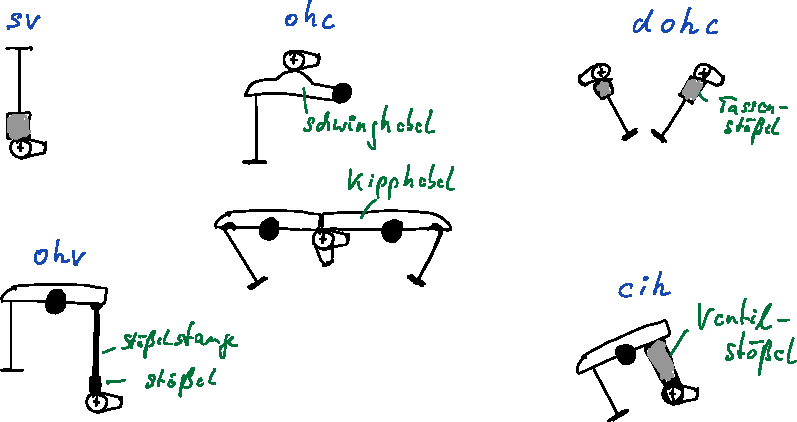
\includegraphics[width=.80\textwidth]{images/01_Anordnung-der-Nockenwelle_Skizze.pdf}%
  \caption{01_Anordnung-der-Nockenwelle_Skizze}%\label{fig:01_Anordnung-der-Nockenwelle_Skizze}%% anpassen
\end{figure}

%\newpage
%\section{01_Generatorregel_Skizze}
%
%01_Generatorregel_Skizze (\autoref{fig:01_Generatorregel_Skizze}).% Referenz
%
\begin{figure}[!hb]% hier: !hb
    \centering
  \includegraphics[width=.80\textwidth]{images/01_Generatorregel_Skizze.pdf}%
  \caption{01_Generatorregel_Skizze}%\label{fig:01_Generatorregel_Skizze}%% anpassen
\end{figure}

%\newpage
%\section{01_Schaltung_Messen_Skizze}
%
%01_Schaltung_Messen_Skizze (\autoref{fig:01_Schaltung_Messen_Skizze}).% Referenz
%
\begin{figure}[!hb]% hier: !hb
    \centering
  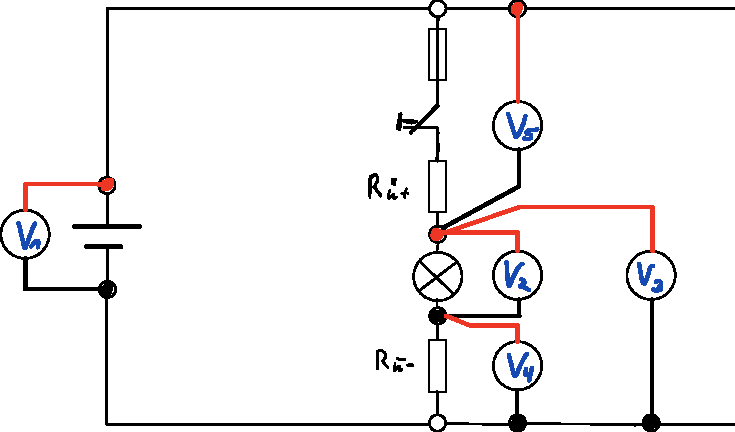
\includegraphics[width=.80\textwidth]{images/01_Schaltung_Messen_Skizze.pdf}%
  \caption{01_Schaltung_Messen_Skizze}%\label{fig:01_Schaltung_Messen_Skizze}%% anpassen
\end{figure}

%\newpage
%\section{01_Verkaufskalkulation_Skizze}
%
%01_Verkaufskalkulation_Skizze (\autoref{fig:01_Verkaufskalkulation_Skizze}).% Referenz
%
\begin{figure}[!hb]% hier: !hb
    \centering
  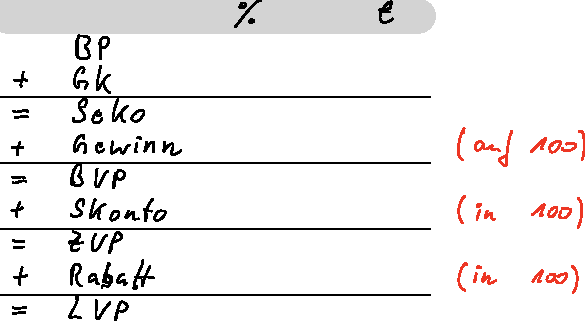
\includegraphics[width=.80\textwidth]{images/01_Verkaufskalkulation_Skizze.pdf}%
  \caption{01_Verkaufskalkulation_Skizze}%\label{fig:01_Verkaufskalkulation_Skizze}%% anpassen
\end{figure}

%\newpage
%\section{02_Motorregel_Skizze}
%
%02_Motorregel_Skizze (\autoref{fig:02_Motorregel_Skizze}).% Referenz
%
\begin{figure}[!hb]% hier: !hb
    \centering
  \includegraphics[width=.80\textwidth]{images/02_Motorregel_Skizze.pdf}%
  \caption{02_Motorregel_Skizze}%\label{fig:02_Motorregel_Skizze}%% anpassen
\end{figure}

%\newpage
%\section{02_Nockenformen_Skizze}
%
%02_Nockenformen_Skizze (\autoref{fig:02_Nockenformen_Skizze}).% Referenz
%
\begin{figure}[!hb]% hier: !hb
    \centering
  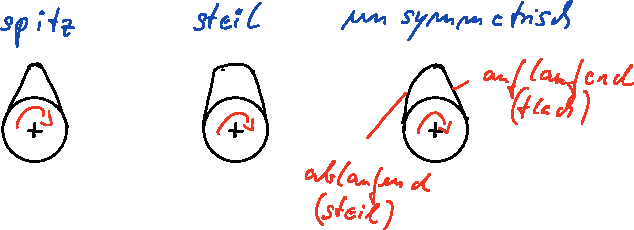
\includegraphics[width=.80\textwidth]{images/02_Nockenformen_Skizze.pdf}%
  \caption{02_Nockenformen_Skizze}%\label{fig:02_Nockenformen_Skizze}%% anpassen
\end{figure}

%\newpage
%\section{02_Schaltung_Messen_Skizze}
%
%02_Schaltung_Messen_Skizze (\autoref{fig:02_Schaltung_Messen_Skizze}).% Referenz
%
\begin{figure}[!hb]% hier: !hb
    \centering
  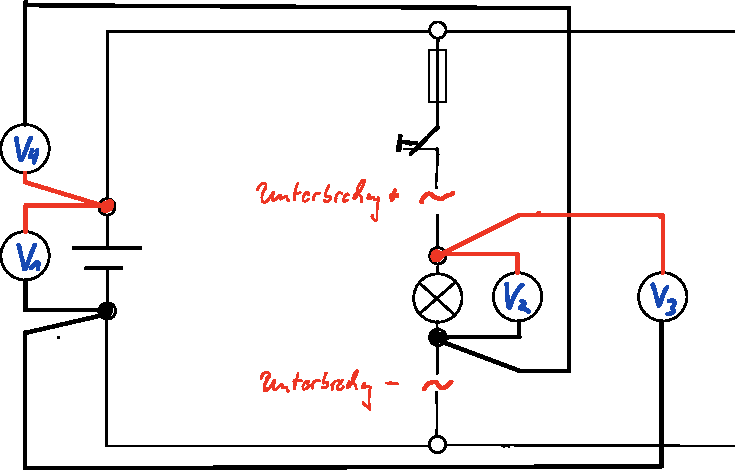
\includegraphics[width=.80\textwidth]{images/02_Schaltung_Messen_Skizze.pdf}%
  \caption{02_Schaltung_Messen_Skizze}%\label{fig:02_Schaltung_Messen_Skizze}%% anpassen
\end{figure}

%\newpage
%\section{02_Umsatzerloese_Skizze}
%
%02_Umsatzerloese_Skizze (\autoref{fig:02_Umsatzerloese_Skizze}).% Referenz
%
\begin{figure}[!hb]% hier: !hb
    \centering
  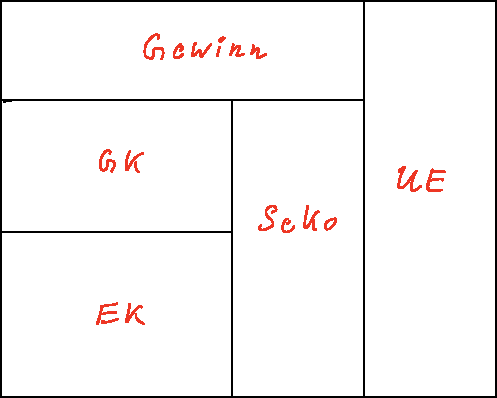
\includegraphics[width=.80\textwidth]{images/02_Umsatzerloese_Skizze.pdf}%
  \caption{02_Umsatzerloese_Skizze}%\label{fig:02_Umsatzerloese_Skizze}%% anpassen
\end{figure}

%\newpage
%\section{03_Arten-von-Ventilbetaetigung_Skizze}
%
%03_Arten-von-Ventilbetaetigung_Skizze (\autoref{fig:03_Arten-von-Ventilbetaetigung_Skizze}).% Referenz
%
\begin{figure}[!hb]% hier: !hb
    \centering
  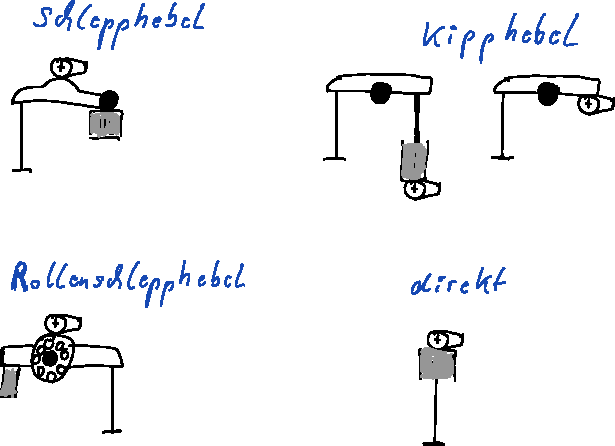
\includegraphics[width=.80\textwidth]{images/03_Arten-von-Ventilbetaetigung_Skizze.pdf}%
  \caption{03_Arten-von-Ventilbetaetigung_Skizze}%\label{fig:03_Arten-von-Ventilbetaetigung_Skizze}%% anpassen
\end{figure}

%\newpage
%\section{03_Kalkulationsfaktor_Skizze}
%
%03_Kalkulationsfaktor_Skizze (\autoref{fig:03_Kalkulationsfaktor_Skizze}).% Referenz
%
\begin{figure}[!hb]% hier: !hb
    \centering
  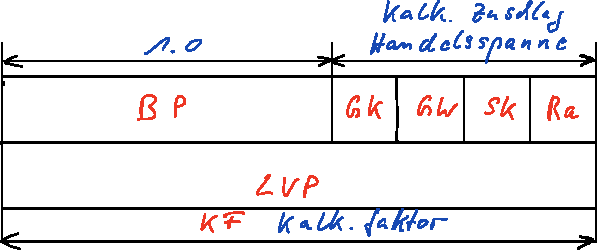
\includegraphics[width=.80\textwidth]{images/03_Kalkulationsfaktor_Skizze.pdf}%
  \caption{03_Kalkulationsfaktor_Skizze}%\label{fig:03_Kalkulationsfaktor_Skizze}%% anpassen
\end{figure}

%\newpage
%\section{03_Schaltung_Messen_Skizze}
%
%03_Schaltung_Messen_Skizze (\autoref{fig:03_Schaltung_Messen_Skizze}).% Referenz
%
\begin{figure}[!hb]% hier: !hb
    \centering
  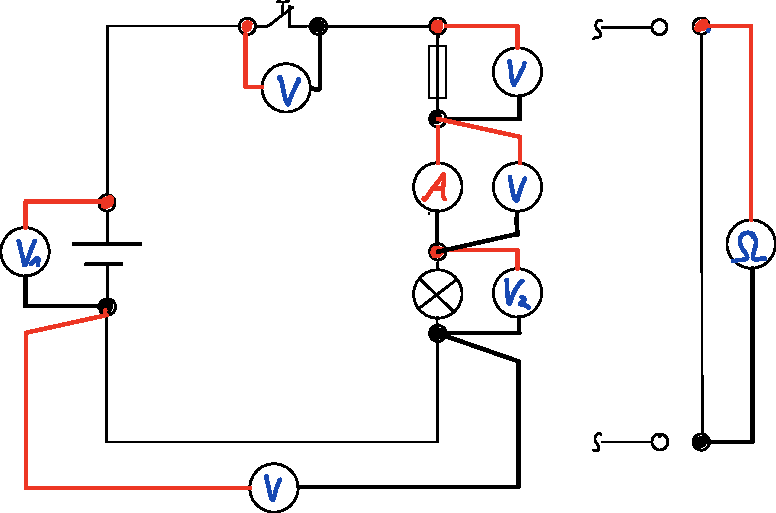
\includegraphics[width=.80\textwidth]{images/03_Schaltung_Messen_Skizze.pdf}%
  \caption{03_Schaltung_Messen_Skizze}%\label{fig:03_Schaltung_Messen_Skizze}%% anpassen
\end{figure}

%\newpage
%\section{03_StromdurchflosseneSpule_Skizze}
%
%03_StromdurchflosseneSpule_Skizze (\autoref{fig:03_StromdurchflosseneSpule_Skizze}).% Referenz
%
\begin{figure}[!hb]% hier: !hb
    \centering
  \includegraphics[width=.80\textwidth]{images/03_StromdurchflosseneSpule_Skizze.pdf}%
  \caption{03_StromdurchflosseneSpule_Skizze}%\label{fig:03_StromdurchflosseneSpule_Skizze}%% anpassen
\end{figure}

%\newpage
%\section{04_Stromdichte_Skizze}
%
%04_Stromdichte_Skizze (\autoref{fig:04_Stromdichte_Skizze}).% Referenz
%
\begin{figure}[!hb]% hier: !hb
    \centering
  \includegraphics[width=.80\textwidth]{images/04_Stromdichte_Skizze.pdf}%
  \caption{04_Stromdichte_Skizze}%\label{fig:04_Stromdichte_Skizze}%% anpassen
\end{figure}

%\newpage
%\section{04_Ventilspielausgleich_Skizze}
%
%04_Ventilspielausgleich_Skizze (\autoref{fig:04_Ventilspielausgleich_Skizze}).% Referenz
%
\begin{figure}[!hb]% hier: !hb
    \centering
  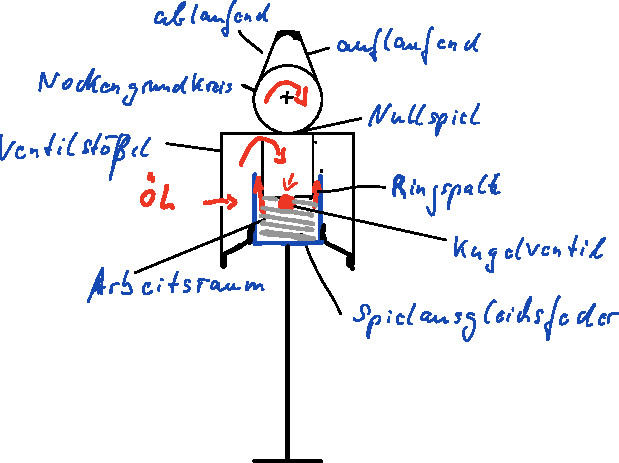
\includegraphics[width=.80\textwidth]{images/04_Ventilspielausgleich_Skizze.pdf}%
  \caption{04_Ventilspielausgleich_Skizze}%\label{fig:04_Ventilspielausgleich_Skizze}%% anpassen
\end{figure}

%\newpage
%\section{05_Dreiventiltechnik_Skizze}
%
%05_Dreiventiltechnik_Skizze (\autoref{fig:05_Dreiventiltechnik_Skizze}).% Referenz
%
\begin{figure}[!hb]% hier: !hb
    \centering
  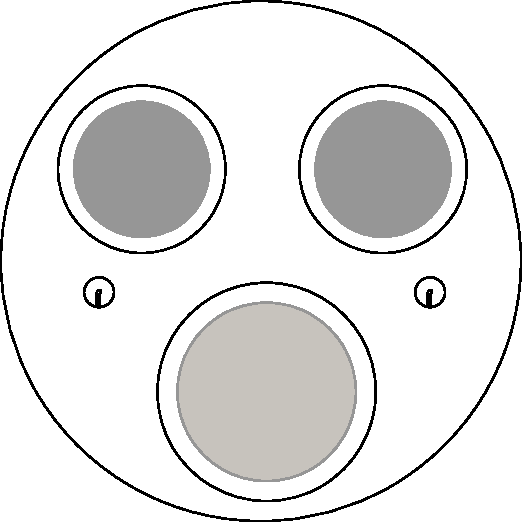
\includegraphics[width=.80\textwidth]{images/05_Dreiventiltechnik_Skizze.pdf}%
  \caption{05_Dreiventiltechnik_Skizze}%\label{fig:05_Dreiventiltechnik_Skizze}%% anpassen
\end{figure}

%\newpage
%\section{05_StromdurchflossenerLeiter_Skizze}
%
%05_StromdurchflossenerLeiter_Skizze (\autoref{fig:05_StromdurchflossenerLeiter_Skizze}).% Referenz
%
\begin{figure}[!hb]% hier: !hb
    \centering
  \includegraphics[width=.80\textwidth]{images/05_StromdurchflossenerLeiter_Skizze.pdf}%
  \caption{05_StromdurchflossenerLeiter_Skizze}%\label{fig:05_StromdurchflossenerLeiter_Skizze}%% anpassen
\end{figure}

%\newpage
%\section{06_Stromfluss_Messen_Skizze}
%
%06_Stromfluss_Messen_Skizze (\autoref{fig:06_Stromfluss_Messen_Skizze}).% Referenz
%
\begin{figure}[!hb]% hier: !hb
    \centering
  \includegraphics[width=.80\textwidth]{images/06_Stromfluss_Messen_Skizze.pdf}%
  \caption{06_Stromfluss_Messen_Skizze}%\label{fig:06_Stromfluss_Messen_Skizze}%% anpassen
\end{figure}

%\newpage
%\section{07_Reihenschaltung_Widerstaende_Skizze}
%
%07_Reihenschaltung_Widerstaende_Skizze (\autoref{fig:07_Reihenschaltung_Widerstaende_Skizze}).% Referenz
%
\begin{figure}[!hb]% hier: !hb
    \centering
  \includegraphics[width=.80\textwidth]{images/07_Reihenschaltung_Widerstaende_Skizze.pdf}%
  \caption{07_Reihenschaltung_Widerstaende_Skizze}%\label{fig:07_Reihenschaltung_Widerstaende_Skizze}%% anpassen
\end{figure}

%\newpage
%\section{08_Relais_Skizze}
%
%08_Relais_Skizze (\autoref{fig:08_Relais_Skizze}).% Referenz
%
\begin{figure}[!hb]% hier: !hb
    \centering
  \includegraphics[width=.80\textwidth]{images/08_Relais_Skizze.pdf}%
  \caption{08_Relais_Skizze}%\label{fig:08_Relais_Skizze}%% anpassen
\end{figure}

%\newpage
%\section{09_Stroeme_einer_Relaisschaltung_Skizze}
%
%09_Stroeme_einer_Relaisschaltung_Skizze (\autoref{fig:09_Stroeme_einer_Relaisschaltung_Skizze}).% Referenz
%
\begin{figure}[!hb]% hier: !hb
    \centering
  \includegraphics[width=.80\textwidth]{images/09_Stroeme_einer_Relaisschaltung_Skizze.pdf}%
  \caption{09_Stroeme_einer_Relaisschaltung_Skizze}%\label{fig:09_Stroeme_einer_Relaisschaltung_Skizze}%% anpassen
\end{figure}

%\newpage
%\section{10_Stromrelais_Skizze}
%
%10_Stromrelais_Skizze (\autoref{fig:10_Stromrelais_Skizze}).% Referenz
%
\begin{figure}[!hb]% hier: !hb
    \centering
  \includegraphics[width=.80\textwidth]{images/10_Stromrelais_Skizze.pdf}%
  \caption{10_Stromrelais_Skizze}%\label{fig:10_Stromrelais_Skizze}%% anpassen
\end{figure}

%\newpage
%\section{11_Schrittrelais_Skizze}
%
%11_Schrittrelais_Skizze (\autoref{fig:11_Schrittrelais_Skizze}).% Referenz
%
\begin{figure}[!hb]% hier: !hb
    \centering
  \includegraphics[width=.80\textwidth]{images/11_Schrittrelais_Skizze.pdf}%
  \caption{11_Schrittrelais_Skizze}%\label{fig:11_Schrittrelais_Skizze}%% anpassen
\end{figure}

%\newpage
%\section{12_Reedkontaktschalter_Skizze}
%
%12_Reedkontaktschalter_Skizze (\autoref{fig:12_Reedkontaktschalter_Skizze}).% Referenz
%
\begin{figure}[!hb]% hier: !hb
    \centering
  \includegraphics[width=.80\textwidth]{images/12_Reedkontaktschalter_Skizze.pdf}%
  \caption{12_Reedkontaktschalter_Skizze}%\label{fig:12_Reedkontaktschalter_Skizze}%% anpassen
\end{figure}

%\newpage
%\section{13_Spannungsverlust_Skizze}
%
%13_Spannungsverlust_Skizze (\autoref{fig:13_Spannungsverlust_Skizze}).% Referenz
%
\begin{figure}[!hb]% hier: !hb
    \centering
  \includegraphics[width=.80\textwidth]{images/13_Spannungsverlust_Skizze.pdf}%
  \caption{13_Spannungsverlust_Skizze}%\label{fig:13_Spannungsverlust_Skizze}%% anpassen
\end{figure}

%\newpage
%\section{14_ Innenwiderstand_von_Spannungsquellen_Skizze}
%
%14_ Innenwiderstand_von_Spannungsquellen_Skizze (\autoref{fig:14_ Innenwiderstand_von_Spannungsquellen_Skizze}).% Referenz
%
\begin{figure}[!hb]% hier: !hb
    \centering
  \includegraphics[width=.80\textwidth]{images/14_ Innenwiderstand_von_Spannungsquellen_Skizze.pdf}%
  \caption{14_ Innenwiderstand_von_Spannungsquellen_Skizze}%\label{fig:14_ Innenwiderstand_von_Spannungsquellen_Skizze}%% anpassen
\end{figure}

%\newpage
%\section{15_Schaltzeichen_Widerstand_Skizze}
%
%15_Schaltzeichen_Widerstand_Skizze (\autoref{fig:15_Schaltzeichen_Widerstand_Skizze}).% Referenz
%
\begin{figure}[!hb]% hier: !hb
    \centering
  \includegraphics[width=.80\textwidth]{images/15_Schaltzeichen_Widerstand_Skizze.pdf}%
  \caption{15_Schaltzeichen_Widerstand_Skizze}%\label{fig:15_Schaltzeichen_Widerstand_Skizze}%% anpassen
\end{figure}

%\newpage
%\section{16_Widerstandsmessung_Skizze}
%
%16_Widerstandsmessung_Skizze (\autoref{fig:16_Widerstandsmessung_Skizze}).% Referenz
%
\begin{figure}[!hb]% hier: !hb
    \centering
  \includegraphics[width=.80\textwidth]{images/16_Widerstandsmessung_Skizze.pdf}%
  \caption{16_Widerstandsmessung_Skizze}%\label{fig:16_Widerstandsmessung_Skizze}%% anpassen
\end{figure}

%\newpage
%\section{17_Leistungsteilung_Skizze}
%
%17_Leistungsteilung_Skizze (\autoref{fig:17_Leistungsteilung_Skizze}).% Referenz
%
\begin{figure}[!hb]% hier: !hb
    \centering
  \includegraphics[width=.80\textwidth]{images/17_Leistungsteilung_Skizze.pdf}%
  \caption{17_Leistungsteilung_Skizze}%\label{fig:17_Leistungsteilung_Skizze}%% anpassen
\end{figure}

%\newpage
%\section{18_Stromflusserhoehung_Strombegrenzung_Spannungsteilung_Skizze}
%
%18_Stromflusserhoehung_Strombegrenzung_Spannungsteilung_Skizze (\autoref{fig:18_Stromflusserhoehung_Strombegrenzung_Spannungsteilung_Skizze}).% Referenz
%
\begin{figure}[!hb]% hier: !hb
    \centering
  \includegraphics[width=.80\textwidth]{images/18_Stromflusserhoehung_Strombegrenzung_Spannungsteilung_Skizze.pdf}%
  \caption{18_Stromflusserhoehung_Strombegrenzung_Spannungsteilung_Skizze}%\label{fig:18_Stromflusserhoehung_Strombegrenzung_Spannungsteilung_Skizze}%% anpassen
\end{figure}

%\newpage
%\section{19_Parallelschaltung_Widerstaende_Skizze}
%
%19_Parallelschaltung_Widerstaende_Skizze (\autoref{fig:19_Parallelschaltung_Widerstaende_Skizze}).% Referenz
%
\begin{figure}[!hb]% hier: !hb
    \centering
  \includegraphics[width=.80\textwidth]{images/19_Parallelschaltung_Widerstaende_Skizze.pdf}%
  \caption{19_Parallelschaltung_Widerstaende_Skizze}%\label{fig:19_Parallelschaltung_Widerstaende_Skizze}%% anpassen
\end{figure}

%\newpage
%\section{28_FT_Brueckenschaltung}
%
%28_FT_Brueckenschaltung (\autoref{fig:28_FT_Brueckenschaltung}).% Referenz
%
\begin{figure}[!hb]% hier: !hb
    \centering
  \includegraphics[width=.80\textwidth]{images/28_FT_Brueckenschaltung.pdf}%
  \caption{28_FT_Brueckenschaltung}%\label{fig:28_FT_Brueckenschaltung}%% anpassen
\end{figure}

%\newpage
%\section{28_FT_Potentialbestimmung}
%
%28_FT_Potentialbestimmung (\autoref{fig:28_FT_Potentialbestimmung}).% Referenz
%
\begin{figure}[!hb]% hier: !hb
    \centering
  \includegraphics[width=.80\textwidth]{images/28_FT_Potentialbestimmung.pdf}%
  \caption{28_FT_Potentialbestimmung}%\label{fig:28_FT_Potentialbestimmung}%% anpassen
\end{figure}

%\newpage
%\section{Messmethodik_Schaltkreis}
%
%Messmethodik_Schaltkreis (\autoref{fig:Messmethodik_Schaltkreis}).% Referenz
%
\begin{figure}[!hb]% hier: !hb
    \centering
  \includegraphics[width=.80\textwidth]{images/Messmethodik_Schaltkreis.pdf}%
  \caption{Messmethodik_Schaltkreis}%\label{fig:Messmethodik_Schaltkreis}%% anpassen
\end{figure}

%\newpage

%\chapter{Quellcode-files}
%% ---------------------------------
% Quellcode 'code/' in Latex speichern. 
% 'archiv/Quellcode-files.tex' 
% HTML, Python, Bash, C, C++, TeX 
% ju 17-Sep-2022 Quellcode-files.tex
% ---------------------------------
%

\section{Python_keywords}

%Python_keywords.py (\autoref{code:Python_keywords-1}).% Referenz
%
\lstset{language=Python}% HTML, Python, Bash, C, C++, TeX
\lstinputlisting[% anpassen
    caption={Quellcode in Python: Python_keywords.py}, %label={code:Python_keywords-1}
]{code/Python_keywords.py}% file

\newpage


%%%%%%%%%%%%%%%%%%%%%%%%%%%%%%%%%%%%%%%%%%%%%%%%%%

% Tabellen/

%\chapter{PDFs}
%% ju 28-5-22 PDFs.tex 

%\section{Messen}\label{sec:Messen}\index{Messen}


% -------
\section{Messmethodik - Schaltkreis}\label{sec:Messmethodik_Schaltkreis}\index{Messmethodik_Schaltkreis}
\includepdf[pages=-]{Tabellen/PDF/Messmethodik-Schaltkreis.pdf}

% -------
\section{Messprotokoll}\label{sec:Messprotokoll}\index{Messprotokoll}
\includepdf[pages=-]{Tabellen/PDF/Messprotokoll.pdf}







%%%%%%%%%%%%%%%%%%%%%%%%%%%%%%%%%%%%%%%%%%%%%%%%%%

% content/beispiele/tex/

%\chapter{Aufbau-der-Arbeit}
%%\chapter{Aufbau der Arbeit}

Jede Arbeit besteht in der Regel aus einer \textbf{Problemstellung}, einem \textbf{definitorischen Abschnitt}, der eigentlichen \textbf{Behandlung der Problemstellung} sowie einer \textbf{Zusammenfassung der zentralen Ergebnisse}.

\begin{description}

	\item[Einleitung] Im Zentrum des erstens Teils stehen die Darstellung des Themas der Arbeit und die genaue Auflistung der Fragestellungen (Wieso ist das Thema relevant?). Ebenso sollten schon einzelne Aspekte des Problems herausgearbeitet werden. Dabei ist es hilfreich, die zentralen Fragen aufzulisten, die im Rahmen der Arbeit beantwortet werden sollen.
	
	Außerdem sollte ein knapper Überblick gegeben werden, in welchen Schritten die Problembehandlung erfolgt: Hinführung zum Thema, Herleitung und Ausformulierung der Fragestellung, Abgrenzung des Themas (Angabe von Aspekten, die zum Thema gehören, aber ausgeklammert werden) und Aufbau der Arbeit (Begründung der Gliederung).
	
	\item[Grundlagen (definitorischer Teil)] Im zweiten Teil sollen zentrale Begriffe definiert und eingeordnet werden. Es geht dabei nicht darum, Definitionen aus Lexika zu suchen; stattdessen sollten problemorientierte Definitionen verwendet werden. Häufig können einzelne Begriffe unterschiedlich weit oder eng definiert werden, sodass auch eine Diskussion unterschiedlicher Definitionsansätze hilfreich sein kann, bevor eine für die weitere Arbeit verbindliche Definition gewählt wird. Zudem sollte ein Überblick über die in der Literatur vorhandenen Methoden bzw. Lösungsansätze, der aktuelle Stand der Technik und verwandte Arbeiten gegeben werden.
	
	\item[Hauptteil] Im Hauptteil der Arbeit (der in der Gliederung selbstverständlich nicht so zu benennen ist\ldots) erfolgt die eigentliche eigentliche Auseinandersetzung mit der Problemstellung. In diesem Teil kommt es darauf an, nicht nur Lehrbuchwissen zusammenzutragen, sondern die Problemstellung reflektiert zu bearbeiteten. Aussagen sollten durch herangezogene Literatur gestützt und belegt werden. Bitte darauf achten, in logischen, nachvollziehbaren Schritten vorzugehen.
	
	\item[Schlussbetrachtung] Die Antwort auf die in der Problemstellung aufgeworfenen Fragen soll kurz und prägnant zusammengefasst werden. Ebenso sollte ein Ausblick auf offen gebliebene Fragen sowie auf interessante Fragestellungen, die sich aus der Arbeit ergeben, gegeben werden. Eine kritische Betrachtung der eigenen Arbeit ist an dieser Stelle ebenfalls sinnvoll.

\end{description}

\noindent
Eine Sammlung unserer Tipps für das Schreiben von Ausarbeitungen befindet sich online unter \url{https://www.dcl.hpi.uni-potsdam.de/media/theses/}.

%\chapter{LaTeX-Beispiel-beamer}
%% ju 23-Jul-21
\section*{Einleitung}

\emph{Sonderzeichen}  wie <<\& oder \%>> müssen mit einem Backslash \verb|\& oder \%| maskiert werden, 
damit sie von LaTeX nicht als Befehle missverstanden werden.


\emph{Website} \footnote{\url{https://golatex.de/wiki/Hauptseite}} \verb|\footnote{\url{https://golatex.de/wiki/Hauptseite}}| 

\emph{PDF Datei einbinden} \verb|\includepdf[landscape=false]{images/logo.eps}| 
\includepdf[landscape=false]{images/logo.eps} 

\clearpage
\subsection*{Stand der Forschung}

Während die traditionelle Latexproduktion bereits hinreichend erforscht ist (\autoref{fig:latex}) \\
\verb|(\autoref{fig:latex})|, bleibt das wissenschaftliche Verständnis elektronischer Verarbeitungsprozesse dieses 
vielseitigen Materials weiterhin lückenhaft. 


\begin{figure}[!ht]% hier: !ht
	\centering
	\includegraphics[width=0.25\textwidth]{images/logo.eps}
	\caption{Traditionelle Latexproduktion}\label{fig:latex}%
\end{figure}

\lstset{language=TeX}% C, TeX, Bash, Python 
\begin{lstlisting}[
	%caption={}, label={code:}%% anpassen
]
% Optionen
scale = Wert, Vergrösserungsfaktor
width/height = Wert für die Einstellung der Breite/Höhe
angle = Wert, Winkel (in Grad)
b = bottom - Seitenende 
t = top - Seitenanfang
h = here
p = page - komplette Seite  
% Abbildung
\begin{figure}[!ht]% hier: !ht
	\centering
	\includegraphics[width=0.25\textwidth]{images/logo.eps}
	\caption{Traditionelle Latexproduktion}\label{fig:latex}%
\end{figure}
\end{lstlisting}


\clearpage
\section*{Methodik}

Unter Zuhilfenahme der Formeln \autoref{eq:ekin} \verb|\autoref{eq:ekin}| und \autoref{eq:impuls} \verb|\autoref{eq:impuls}| werden wir 
diese Forschungslücke schließen.  
$E_{kin}$ \verb|$E_{kin}$| ist die kinetische Energie, $m$ \verb|$m$| die Masse und $\vec{v}$ \verb|$\vec{v}$| die Geschwindigkeit.

Wurzel $\sqrt{2}$ \verb|$\sqrt{2}$|

Bruch $\frac{\text{Zähler}}{\text{Nenner}}$ \verb|$\frac{\text{Zähler}}{\text{Nenner}}$|

\begin{equation}
	\label{eq:ekin}% 
	\sum E_{kin} = \sum E'_{kin}
\end{equation}

\begin{equation}
	\label{eq:impuls}% 
	\vec{v_1} - \vec{v_1'} = \frac{m_2}{m_1} (\vec{v_2'} - \vec{v_2})
\end{equation}

\lstset{language=TeX}% C, TeX, Bash, Python 
\begin{lstlisting}[
	%caption={}, label={code:}%% anpassen
]
% Mathe
\begin{equation}
	\label{eq:ekin}% 
	\sum E_{kin} = \sum E'_{kin}
\end{equation}
\end{lstlisting}


\clearpage
\section*{Ausblick}

Daraus ergeben sich gemäß (\autoref{tab:schritte}) \verb|(\autoref{tab:schritte})| folgende nächste Schritte, 
deren sequenzielle Ausführung von essenzieller Bedeutung ist.

\begin{table}[!ht]% hier: !ht
	\centering
	\begin{tabular}{@{}cl@{}}% lcr
		\toprule
		\textbf{Nr.} & \textbf{Vorgehen} \\
		\midrule
		1 & Aktuellen Forschungsstand recherchieren \\
		2 & Methoden entwickeln \\
		3 & Schlussfolgerung aufstellen \\
		\bottomrule
	\end{tabular}
	\caption{Nächste Schritte}\label{tab:schritte}
\end{table}

\clearpage
\lstset{language=TeX}% C, TeX, Bash, Python 
\begin{lstlisting}[
	%caption={}, label={code:}%% anpassen
]
% Tabelle
\begin{table}[!ht]% hier: !ht
	\centering
	\begin{tabular}{@{}cl@{}}% lcr
		\toprule
		\textbf{Nr.} & \textbf{Vorgehen} \\
		\midrule
		1 & Aktuellen Forschungsstand recherchieren \\
		2 & Methoden entwickeln \\
		3 & Schlussfolgerung aufstellen \\
		\bottomrule
	\end{tabular}
	\caption{Nächste Schritte}\label{tab:schritte}
\end{table}
\end{lstlisting}
%\chapter{Latex-install-Ubuntu}
%% letztes Update: 27-Jul-20
Quelle: Dr.~Uwe Ziegenhagen -- Anleitung zur TEX Live Installation

\section{TEX Live Download}\label{tex-live-download}

Download \footnote{\url{http://mirror.ctan.org/systems/texlive/tlnet}}

Download-texlive vgl.~(\autoref{code:Download-texlive}).

\lstset{language=C}% C, TeX, Bash, Python 
\begin{lstlisting}[%% anpassen
caption={Download-texlive},label={code:Download-texlive}
]
cd Downloads
tar xvfz install-tl-unx.tar.gz
cd install-tl-20200114
perl install-tl
perl install-tl -gui
\end{lstlisting}

\section{TeX Version}\label{tex-version}

tex --version

\section{TEX Live Installation}\label{tex-live-installation}

Install-texlive vgl.~(\autoref{code:Install-texlive}).

\lstset{language=C}% C, TeX, Bash, Python 
\begin{lstlisting}[%% anpassen
caption={Install-texlive},label={code:Install-texlive}
]
sudo apt install texlive texlive-latex-recommended texlive-fonts-recommended \
    texlive-latex-base texlive-base texlive-latex-extra texlive-lang-german

# Verbesserte Schriftarten bei T1-Kodierung
sudo apt-get install cm-super 
\end{lstlisting}

\section{Umgebungsvariablen für
Unix}\label{umgebungsvariablen-fuer-unix}

Umgebungsvariable vgl.~(\autoref{code:Umgebungsvariable}).

\lstset{language=C}% C, TeX, Bash, Python 
\begin{lstlisting}[%% anpassen
caption={Umgebungsvariable},label={code:Umgebungsvariable}
]
vi ~/.profile
# Datei 
PATH=/usr/local/texlive/2019/bin/x86_64-linux:$PATH; export PATH
MANPATH=/usr/local/texlive/2019/texmf-dist/doc/man:$MANPATH; export MANPATH
INFOPATH=/usr/local/texlive/2019/texmf-dist/doc/info:$INFOPATH; export INFOPATH

sudo vi /etc/manpath.config
# Datei 
MANPATH_MAP /usr/local/texlive/2019/bin/x86_64-linux \
  /usr/local/texlive/2019/texmf-dist/doc/man  
\end{lstlisting}

%\chapter{Mathe-Aufgaben}
%
\textbf{Aufgabe 1:} \enspace Jasmin hat ihre Freunde Nico, Laura und Anna zum Geburtstag eingeladen. Nico will nicht kommen, wenn Laura nicht kommt. Laura und Anna kommen beide oder kommen beide nicht. Aber Anna sagt: >>Wenn Nico und Laura beide nicht kommen, dann komme ich.<< Wer von den dreien wird unter diesen Bedingungen tatsächlich zum Geburtstag erscheinen?


\textbf{Aufgabe 2:} \enspace In der Anwaltsserie >>Suits<< (Staffel 4, Folge 1) kommt es zu Folgendem Gespräch zwischen Mike und seiner Sekräterin Amy.


\begin{enumerate}[label={\protect\ding{\value*}},start=192]
    \item Amy: >>Und wie lief dein Treffen mit dem geheimnisvollen Harvey Specter?<<
    \item Mike: >>Ein Arsch zu sein macht einen nicht geheimnisvoll.<<
    \item Amy: >>Na dann bist du ja ein ganz offenes Buch.<<
\end{enumerate}

Untersuchen Sie das Gespräch aussagenlogisch und prüfen Sie den Wahrheitswert von Amys Aussage.


\textbf{Aufgabe 3:} \enspace Formalisieren Sie die folgenden Aussagen und verneinen Sie sie anschließend (ohne das Wort nicht davor zu setzen) und übersetzen Sie wieder in Umgangssprache:

\begin{enumerate}[label=(\alph*)]
    \item Volksmund: >>Bei Nacht sind alle Katzen grau.<<
    \item Plakatwerbung: >>Wenn einer hochguckt, dann gucken alle.<<
    \item Gorbatschov: >>Wer zu spät kommt, den bestraft das Leben.<<
\end{enumerate}

\textbf{Aufgabe 4:} \enspace Wurzel

\begin{multicols}{3}
    \begin{enumerate}[label=(\alph*)]
        \item $\sqrt{169}$
        \item $\sqrt{0,36}$
        \item $\frac{\sqrt{45}}{\sqrt{80}}$
        \item $\sqrt{32}$
        \item $\sqrt{2}$
        \item $\sqrt{1,44}$
        \item $\sqrt{\frac{75}{12}}$
    \end{enumerate}
\end{multicols}
%\chapter{Mathe-Latex}
%\section{\textbf{Text Unterstreichen}}
    \underline{wichtiger Text} und \emph{kursiver Text} und \textbf{fetter Text}

 
\section{\textsc{Kapitaelchen}}  
    Text in Grossbuchstaben setzen durch \LaTeX
    \begin{itemize} % \item[] avoids bullet
        \item[] Einen längeren Satz\\ einrücken.
    \end{itemize}

\section{Vor- und Nachteile}
    \begin{tabular}[h]{ll}
        {\textbf{Vorteile}}   &  {\textbf{Nachteile}} \\
        Argument 1            &  Argument 2 \\
        Argument A            &  Argument B \\
    \end{tabular} 

\section{Summe}
    \begin{tabular}[h]{clrr}
        & Betrag &               &  $1.000,00$ \\
    $-$ & Skonto & $2\%$         &     $20,00$ \\
        \hline
    $=$ & $\sum$ &               &    $980,00$  
    \end{tabular} 
    
\section{Division Zinsen}
    $
        \frac{\text{ Betrag } \cdot \text{ Prozentsatz } \cdot \text{ Zeit } }{100 \cdot \text{ Zeitgröße }} 
        = \frac{12.597,90 \cdot 12 \cdot 20 \text{ T } }{100 \cdot 360} 
        = 83,99 \text{ \euro }
    $

    \begin{align*}
        \frac{\text{ Betrag } \cdot \text{ Prozentsatz } \cdot \text{ Zeit } }{100 \cdot \text{ Zeitgröße }} 
        = \frac{12.597,90 \cdot 12 \cdot 20 \text{ T } }{100 \cdot 360} 
        = 83,99 \text{ \euro }
    \end{align*} 

\section{Tabelle 2}
    \begin{table}[!ht]% hier: !ht 
        \begin{tabular}{@{}lcr@{}}
        \toprule 
        \textbf{Großbuchstaben} & \textbf{Kleinbuchstaben} & \textbf{Name}\\
        \midrule
        21 \euro & 22000 & 230.000 \\
        $31$ \euro & $32000$ & $330.000$ \\
        \bottomrule
        \end{tabular}
    \end{table}

\section{Checkliste}
    Meine Liste
    \begin{itemize} \itemsep -2pt  % reduce space between items
        \item[$\Box$]   Punkt 1
        \item[$\Box$]   Aufgabe 2 
    \end{itemize}

    \begin{itemize}[label=\checkmark] \itemsep -2pt
        \item Check 1
        \item Check 2   
    \end{itemize}

\section{\textcolor{rot5}{Nenne 4x Lerzielstufen (Taxonomien)}}
    \begin{enumerate}[label={\protect\ding{\value*}},start=192]
        \item Reproduktion
        \item Reorganisieren
        \item Transfer
        \item Kreativ
    \end{enumerate}

\section{Wurzel berechnen}
    \begin{multicols}{3}
        \begin{enumerate}[label=(\alph*)]
            \item $\sqrt{169}$
            \item $\sqrt{0,36}$
            \item $\frac{\sqrt{45}}{\sqrt{80}}$
        \end{enumerate}
    \end{multicols}

\section{Aufgabe Logik}
    Formalisieren Sie die folgenden Aussagen und verneinen Sie sie anschließend (ohne das Wort nicht davor zu setzen) und übersetzen Sie wieder in Umgangssprache:

    \begin{enumerate}[label=(\alph*)]
        \item Volksmund: >>Bei Nacht sind alle Katzen grau.<<
        \item Plakatwerbung: >>Wenn einer hochguckt, dann gucken alle.<<
        \item Gorbatschov: >>Wer zu spät kommt, den bestraft das Leben.<<
    \end{enumerate}

\section{Quotientenregel}
    \begin{itemize} % \item[] ohne bullet
        \item[] $\left(\frac{u}{v}\right)^{\prime} = \frac{u^{\prime} \cdot v-u \cdot v^{\prime}}{v^{2}}$
        
        \item[] $\frac{\text{ Ableiten } \cdot \text{ Stehen lassen } - \text{ Stehen lassen } \cdot \text{ Ableiten }}{\text{ Nenner}^2}$
    \end{itemize}

    
\section{Logarithmus}
    \begin{align}
        ln(a \cdot b)   &= ln(a) + ln(b) \\
        ln(\frac{a}{b}) &= ln(a) - ln(b) \\
        ln(a^b)         &= b \cdot ln(a)
    \end{align}

    \newpage
\section{\LaTeX - Assistent}
    Formeleditor~\footnote{\url{https://www.matheretter.de/rechner/latex}}
    \begin{align}
        \text{ Matrix }       &= \begin{pmatrix} a & b \\ c & d \end{pmatrix} \\
        \text{ Vektor }       &= \begin{pmatrix} x\\y \end{pmatrix} \\
        \text{ Vektorbuchstabe } &= \vec{x} \\
        \text{ Wurzel }       &= \sqrt[n]{a} \text{ Potenz } a^{b} \\
        \text{ Bruch }        &= \frac{a}{b} \\
        \text{ Log }          &= \log_{b}{a} \\
        \text{ Summe }        &= \sum \limits_{n=0}^{\infty} \\
        \text{ Index }        &= x_{1,2} \\
        \text{ Klammern }     &= \left\{x, y\right\} \\
        \text{ Alphabet kl. } &= +\\%α β γ δ ε ζ η θ ι κ λ μ ν ξ ο π ρ σ τ υ φ χ ψ ω \\
        \text{ Alphabet gr. } &= +\\%Α Β Γ Δ Ε Ζ Η Θ Ι Κ Λ Μ Ν Ξ Ο Π Ρ Σ Τ Υ Φ Χ Ψ Ω \\
        \text{ Element }      &= \in \notin \sum \quad \prod \quad () \quad \to \quad \infty\\
        \text{ Mengen }       &= \mathbb{N} \mathbb{Z} \mathbb{Q} \mathbb{R} \mathbb{I} \mathbb{C} \mathbb{L} \\
        \text{ Relation }     &= < > \geq \leq \neq \subset \subseteq \approx \in \supset \supseteq \notin \\
        \text{ Pfeile }       &= +\\%\rightarrow \leftarrow \Longleftrightarrow \Longrightarrow \Longleftarrow \\
    \end{align}

\section{Formeln in einer Zeile}
    $
        u = \bar{u} + \epsilon \cdot u_1 \quad
        v = \bar{v} + \epsilon \cdot v_1 \quad
        w = \bar{w} + \epsilon \cdot w_1 \quad
    $

    $
        \left( \begin{array}{rrr}
            1 & 0 & 0 \\                                              
            0 & 1 & 0 \\
            0 & 0 & 1 \\                                              
        \end{array}\right)
    $

\section{Sonderzeichen}
    \textbackslash \{...\} \$ \& \# \textdegree \^{} \_ \textasciitilde \%

\section{Währungszeichen}
    \euro 100 \textdollar 100 \textsterling 100 $1.000,00 \text{ \euro }$ 1.000,00 \euro

\section{Leerzeichen}
\begin{itemize} % \item[] avoids bullet
    \item[] [a\,b] ($0.16667em$)
    \item[] [a\:b] ($0.2222em$)
    \item[] [a\enspace b] ($0.5em$)
    \item[] [a\quad b] ($1em$)
    \item[] [a\hspace{5em} b] (5em)
\end{itemize}

\newpage
\section{Griechisches Alphabet}
    \begin{table}[!ht]% hier: !ht 
        \begin{tabular}{@{}ccl@{}}
        \toprule 
        \textbf{Großbuchstaben} & \textbf{Kleinbuchstaben} & \textbf{Name}\\
        \midrule
        A & $\alpha$ & Alpha\\
        B & $\beta$ & Beta\\
        $\Gamma$ & $\gamma$ & Gamma \\
        $\Delta$ & $\delta$ & Delta\\
        E & $\epsilon$, $\varepsilon$ & Epsilon\\
        Z & $\zeta$ & Zeta\\
        H & $\eta$ & Eta\\
        $\Theta$ & $\theta$, $\vartheta$ & Theta\\
        I & $\iota$ & Iota\\
        K & $\kappa$, $\varkappa$ & Kappa\\
        $\Lambda$ & $\lambda$ & Lambda\\
        M & $\mu$ & My\\
        N & $\nu$ & Ny\\
        $\Xi$ & $\xi$ & Xi\\
        O & o & Omikron\\
        $\Pi$ & $\pi$, $\varpi$ & Pi\\
        P & $\rho$, $\varrho$ & Rho\\
        $\Sigma$ & $\sigma$, $\varsigma$ & Sigma\\
        T & $\tau$ & Tau\\
        Y & $\upsilon$ & Ypsilon\\
        $\Phi$ & $\phi$, $\varphi$ & Phi\\
        X & $\chi$ & Chi\\
        $\Psi$ & $\psi$ & Psi\\
        $\Omega$ & $\omega$ & Omega\\
        \bottomrule
        \end{tabular}
    \end{table}

\section{Tabelle 3}
    Tabellengenerator~\footnote{\url{https://www.tablesgenerator.com/}} 
    und Rechner~\footnote{\url{https://www.matheretter.de/rechner/latex}}

    \begin{multicols}{2}
        \begin{tabular}[h]{ll|l}
            &  A     & B     \\ 
        \hline
        1)* &  $a_1$ & $b_1$ \\
        2)  &  $a_2$ & $b_2$ \\
        3)  &  $a_3$ & $b_3$ 
        \end{tabular}
        
        \columnbreak% Spalte
        *Beachte: $\sqrt[n]{x} = x^\frac{1}{n}$       
    \end{multicols}

\section{Tabelle und Grafik}
    \begin{multicols}{2}
        \begin{tabular}[h]{l|c|r}
            Spalte 1 & Spalte 2 & Spalte 3 \\
            \hline
            heise & tipps & tricks \\
        \end{tabular}    

        \columnbreak% Spalte

        \includegraphics[width=2.0cm]{images/logo.eps}% Logo   
    \end{multicols}  

\newpage
\section{Farben}
    \begin{testcolors}[rgb,cmyk,HTML,gray]
        \testcolor{black}
        \testcolor{white}
        \testcolor{darkgray}
        \testcolor{gray}
        \testcolor{lightgray}
        \testcolor{red}
        \testcolor{green}
        \testcolor{blue}
        \testcolor{cyan}
        \testcolor{magenta}
        \testcolor{yellow}
        \testcolor{brown}
        \testcolor{lime}
        \testcolor{olive}
        \testcolor{orange}
        \testcolor{pink}
        \testcolor{purple}
        \testcolor{teal}
        \testcolor{violet}
        \testcolor{rot5}
        \testcolor{blau5}  
        \testcolor{grau2}    
        \testcolor{orange}                       
    \end{testcolors}
    
\section{Farbenfolgen}
    \definecolorseries{test}{rgb}{step}[rgb]{.95,.85,.55}{.17,.47,.37}
    \definecolorseries{test}{hsb}{step}[hsb]{.575,1,1}{.11,-.05,0}
    \definecolorseries{test}{rgb}{grad}[rgb]{.95,.85,.55}{3,11,17}
    \definecolorseries{test}{hsb}{grad}[hsb]{.575,1,1}{.987,-.234,0}
    \definecolorseries{test}{rgb}{last}[rgb]{.95,.85,.55}[rgb]{.05,.15,.55}
    \definecolorseries{test}{hsb}{last}[hsb]{.575,1,1}[hsb]{-.425,.15,1}
    \definecolorseries{test}{rgb}{last}{red!50}{blue}
    \definecolorseries{test}{hsb}{last}{yellow!50}{black}
    \definecolorseries{test}{cmy}{last}{orange!50}{green}

    \resetcolorseries[12]{test}
    \rowcolors[\hline]{1}{test!!+}{test!!+}
    \setlength{\tabcolsep}{5mm} % Abstände zwischen den Spalten
    \begin{tabular}[h]{c||c||c||c||c||c||c||c||c||c}
        $S_1$ & $S_2$ & $G_1$ & $G_2$ & $L_1$ & $L_2$ & $L_3$ & $L_4$ & $L_5$ \\
        \hline \hline
        \number\rownum & \number\rownum & \number\rownum & \number\rownum & \number\rownum & \number\rownum & \number\rownum & \number\rownum & \number\rownum \\
        \number\rownum & \number\rownum & \number\rownum & \number\rownum & \number\rownum & \number\rownum & \number\rownum & \number\rownum & \number\rownum \\
        \number\rownum & \number\rownum & \number\rownum & \number\rownum & \number\rownum & \number\rownum & \number\rownum & \number\rownum & \number\rownum \\
        \number\rownum & \number\rownum & \number\rownum & \number\rownum & \number\rownum & \number\rownum & \number\rownum & \number\rownum & \number\rownum \\
        \number\rownum & \number\rownum & \number\rownum & \number\rownum & \number\rownum & \number\rownum & \number\rownum & \number\rownum & \number\rownum \\
        \number\rownum & \number\rownum & \number\rownum & \number\rownum & \number\rownum & \number\rownum & \number\rownum & \number\rownum & \number\rownum \\
        \number\rownum & \number\rownum & \number\rownum & \number\rownum & \number\rownum & \number\rownum & \number\rownum & \number\rownum & \number\rownum \\
        \number\rownum & \number\rownum & \number\rownum & \number\rownum & \number\rownum & \number\rownum & \number\rownum & \number\rownum & \number\rownum \\
        \number\rownum & \number\rownum & \number\rownum & \number\rownum & \number\rownum & \number\rownum & \number\rownum & \number\rownum & \number\rownum \\
        \number\rownum & \number\rownum & \number\rownum & \number\rownum & \number\rownum & \number\rownum & \number\rownum & \number\rownum & \number\rownum \\
        \number\rownum & \number\rownum & \number\rownum & \number\rownum & \number\rownum & \number\rownum & \number\rownum & \number\rownum & \number\rownum \\
        \number\rownum & \number\rownum & \number\rownum & \number\rownum & \number\rownum & \number\rownum & \number\rownum & \number\rownum & \number\rownum \\
        \number\rownum & \number\rownum & \number\rownum & \number\rownum & \number\rownum & \number\rownum & \number\rownum & \number\rownum & \number\rownum \\
        \number\rownum & \number\rownum & \number\rownum & \number\rownum & \number\rownum & \number\rownum & \number\rownum & \number\rownum & \number\rownum \\
        \number\rownum & \number\rownum & \number\rownum & \number\rownum & \number\rownum & \number\rownum & \number\rownum & \number\rownum & \number\rownum \\ 
    \end{tabular}
%\chapter{Sprachlich-formale-Aspekte}
%%\chapter{Sprachlich-formale Aspekte}

Wissenschaftliche Ausarbeitungen dienen der Wissensvermittlung -- es ist überaus wichtig, Lesenden die Informationsaufnahme möglichst einfach zu machen, Inhalte logisch zu gliedern und in guter sprachlicher Form darzustellen.


\section{Textverständlichkeit}

Der Text ist logisch aufzubauen und so zu formulieren, dass er auch für den nicht an der Durchführung der Arbeit beteiligten Lesenden verständlich und nachvollziehbar ist. Die behandelten Themen müssen leicht erkennbar sein. Größere Abschnitte sollten einen kurzen Überblick über ihre Inhalte geben. Die Verständlichkeit des Textes kann durch die Verwendung von kurzen Sätzen, einer einfachen, aber fachsprachlich korrekten Wortwahl und durch die Vermeidung von Füllworten und überflüssigen Fremdworten wesentlich erhöht werden.

\begin{itemize}
\item Keine Prosa, sondern präzise Begriffe und Sätze!
\item Eine einheitliche Terminologie verwenden, damit Begriffe wiedererkannt werden können.
\item Zentrale Begriffe klären und die Arbeit für interessierte Laien verständlich halten.
\item Pure Textblöcke, die sich über mehrere Seiten erstrecken, sind ein Zeichen für mangelnde strukturelle Leseunterstützung. Weiter unterteilen oder variantenreichere Inhaltsarten (Schriftarten, Listen, Diagramme, Tabellen, \ldots) einsetzen.
\item Das schnelle überfliegen des Textes und das Springen in der Arbeit muss aktiv unterstützt werden. Lesende müssen jederzeit die wesentlichen gerade diskutierten Themen schnell erkennen und auch bestimmte vorher schon einmal gelesene Fakten schnell wiederfinden können.
\item Kurz einen Gesamtüberblick (Einordnung ins >>große Bild<<, eine Tabelle) geben und dann tiefer in die Details. Z. B. vor dem Start einer Reihe von Subsections die verschiedene Ausprägungen eines Sachverhalts diskutieren, diese Sachverhalte vorher alle aufzählen und kurz erläutern.
\item Fremdworte/Fachbegriffe nicht einfach ohne weitere Erläuterung verwenden und als bekannt voraussetzen. Selbst wenn der Begriff etabliert und bekannt scheint -- das ist oft auch nur in einem Teilgebiet (der Informatik) so. Deshalb generell Fachbegriffe und Fremdworte erläutern.
\item Die einzelnen Abschnitte sollten entsprechend auf einander verweisen. Überleitungen und Zusammenfassungen zwischen Kapiteln sind hilfreich.
\item Zu Beginn eines Kapitels ist eine Übersicht über dessen Inhalt sinnvoll. Am Ende eines Kapitels kann eine Überleitung zum nächsten Kapitel helfen, den roten Faden aufzuzeigen.
\item Gute Überschriften, vielseitige Präsentation der Inhalte (Diagramme, Tabellen, Auflistungen, \ldots) und aussagekräftige Inhaltsunterschriften verwenden.
\item Durch eine Kombination aus Text und Bild lassen sich komplexe Sachverhalte vereinfacht darstellen und verständlich vermitteln.
\item Verwendet sprechende Titel für Kapitel/Sections/\ldots! Nicht einfach nur >>Aufbau<<, >>Mechanismen<<, >>Dritter Schritt<<, etc. Man sollte nicht erst den Text lesen müssen, um den Kontext zu verstehen. Viel besser: >>Aufbau einer Ausführungsumgebung für Microservices<<, >>Mechanismen zur Fehlervermeidung und Fehlerbeseitigung<<, >>Dritter Schritt: Implementierung der Schnittstellen zwischen Diensten<<.
\item Statt in der Textform z. B. >>mittels einerseits \ldots andererseits<<,\\>>erstens\ldots zweitens\ldots drittens<< o. ä. lieber Aufzählungszeichen verwenden. Dies unterstützt die Lesbarkeit teilweise enorm.
\item Möglichkeiten zur Hervorhebung (z. B. Fettdruck) und Textstrukturierung (Gedankenstriche, Klammern, Semikolon, Doppelpunkt, \ldots) nutzen.
\end{itemize}



\section{Ausdruck \& Stil}

Eine wissenschaftliche Ausdrucksweise ist sachlich, präzise und bemüht sich um Objektivität. Die Verwendung umgangssprachlicher Ausdrücke, schwammiger Formulierungen und übertriebener literarischer Stilmittel (z. B. Verwendung von Synonymen) stören die wissenschaftliche Ausdrucksweise.

\begin{itemize}
\item Umgangssprachliche Formulierungen vermeiden (>>von vorneherein<<, >>wird es richtig teuer<<, >>ziemlich simpel<<, >>Gehen wir das ganze einmal durch<<, >>zum Laufen zu bringen<<, >>sprich\ldots<<, >>Fazit: \ldots<<, >>Ich habe mir gedacht,\ldots<<)
\item Komponenten nicht personifizieren (>>der JBoss/er<<, >>die Apaches<<, >>JBosse<<).
\item    Vermeidet das Wort >>offensichtlich<<. Das wirkt, als hieltet ihr die Lesenden für dumm.
\item    Vermeidet Füllwörter wie >>sehr<<. Wenn etwas >>sehr wichtig<< ist, dann sind in der Schriftsprache Worte wie >>zentral<<, >>fundamental<<, >>essentiell<<, etc. eleganter.
\item    Worte wie >>sehr<<, >>relativ<<, >>ziemlich<<, >>quasi<<, >>gewissermaßen<< sind in den allermeisten Fällen überflüssig und ungenau.
\item    Die Begriffe, für die Demonstrativpronomen (dieser/jener/welcher) Stellvertreter sind, müssen eindeutig erkennbar sein.
\item    Nicht zu umständliche Stellvertreterausdrücke verwenden (>>der zur Diskussion stehende Sachverhalt<<, >>die vorbezeichneten Gegenstände<<, etc.) -- da müssen Lesende viel zu viel nachdenken (und erstmal den Lesefluss stoppen und nachgucken, welche drei Sachen eigentlich gemeint sind).
\item    Nicht verschiedenste Synonyme für ein und denselben Begriff verwenden -- insbesondere, wenn der Begriff etabliert ist (Negativbeispiel: >>künstliche neuronale Netze<<, >>artifizielle Netze<<, >>die in Rede stehenden Netze<<, >>ebenjene Netze<<, >>die beschriebenen Netze<<)
\end{itemize}



\section{Rechtschreibung \& Grammatik}

Mindestens ebenso wichtig wie die Verständlichkeit ist die sprachliche Korrektheit. Ausarbeitungen müssen hinsichtlich Rechtschreibung, Grammatik, Satzbau und Zeichensetzung ohne Fehler sein. Ein nennenswerter Fehleranteil wird oft als Indikator für mangelnde Sorgfalt und Ernsthaftigkeit der Arbeit gewertet. Solche Arbeiten werden nicht anerkannt auch nicht als Vor-Version!).

\begin{itemize}
\item Alles, was die Rechtschreibkontrolle nicht kennt, ist entweder falsch geschrieben oder muss als Fremdwort, Eigenname, \verb|\code| etc. hervorgehoben sein.
\item Es empfiehlt sich generell, Freunde, Kommilitonen, und eine Software zur Prüfung der Rechtschreibung \& Grammatik nochmal auf den Text schauen zu lassen. Als Autor bekommt man schnell einen Tunnelblick und sieht die Fehler nicht mehr.
\item Beachtet schwierige Wörter. >>zum einen<<, >>zum anderen<<, >>des Weiteren<<
\item Regeln für das Setzen von Bindestrichen: Deutsch > immer (>>Hasso-Plattner-Institut<<), Englisch > in der Regel nicht (>>Hasso Plattner Institute<<), Deutsch+Englisch > kombiniert (>>Java EE-Sicherheitsmodell<<). Im Deutschen kommt es äußerst selten vor, dass Worte weder Bindestrich haben noch zusammengeschrieben werden können. Es heißt z. B. nicht >>Download Modus<<, sondern >>Download-Modus<< oder (da Download im Duden steht) >>Downloadmodus<<.
\item Zu einem >>einerseits<< muss es ein >>andererseits<< geben, zu einem >>erstens<< auch ein >>zweitens<<, zu einem >>sowohl<< auch ein >>als auch<<, usw.
\end{itemize}

Schreibung von Zahlen (deutsch):

\begin{itemize}
\item Zahlen von eins bis zwölf werden in der Regel ausgeschrieben. Ansonsten nur ein- und zweisilbige Zahlwörter (hundert, tausend, \ldots)
\item Vor Zeichen, Abkürzungen von Maßen, Gewichten, Geldsorten usw. ist die Zahl in Ziffern zu schreiben: 3 km; 7,4 kg; 6 EUR. Steht statt der Abkürzung die entsprechende Vollform, kann man sowohl in Ziffern als auch in Buchstaben schreiben: 11 Kilometer/elf Kilometer; 2 Euro/zwei Euro.
\item Die Zahlen von 13 an können -- sofern sie Übersichtlich sind -- auch ausgeschrieben werden.
\item Im IT-Bereich gibt es sehr oft einen Unterschied zwischen 0 (dem Zahlenwert) und null (dem Nullwert/NIL, Fehlen eines Wertes)!
\item Zahlen sollten zur besseren Lesbarkeit in Dreiergruppen gegliedert werden, und zwar sowohl links als auch rechts des Dezimaltrennzeichens. Laut ISO 80000 soll das Tausendertrennzeichen ein schmales Leerzeichen sein, niemals ein Komma, Punkt oder irgendein anderes Zeichen. Zahlen sollten (außer bei tabellarischer Darstellung) erst ab fünf Stellen untergliedert werden.
\item Sätze nie mit Konjunktionen (>>und<<, >>oder<<, >>aber<<, sondern) beginnen. Konjunktionen sind -- wie der Name schon sagt -- Verbindungswörter und stellen die syntaktische Verbindung zwischen Wörtern, Satzteilen oder Sätzen her.
\end{itemize}


\section{Grafiken, Tabellen \& Codeausschnitte}

Jede Fließumgebung (Grafiken, Graphen, Diagramme, Tabellen, Codeausschnitte, \ldots) muss beschriftet sein (>>captions<<).

\begin{itemize}
\item Die Beschreibungen der Abbildungen, Tabellen, Diagramme, Quellcode, etc. müssen jene auch ohne Kontext beschreiben -- erläutern, was man alles sehen und erkennen kann. So muss man beim Betrachten nicht zurück in den Fließtext springen.
\item In jeder Beschriftung müssen folgende Fragen beantwortet werden: Was ist dargestellt? Welche Besonderheiten sind zu erkennen? Welche Rückschlüsse ergeben sich daraus für den momentan behandelten Sachverhalt?
\item Die Achsen von Diagrammen ordentlich beschriften (Metrik und Einheiten). Bei Vergleichen angeben, ob große oder ob kleine Werte besser sind. Fehlerbalken verwenden.
\item Wenn Text in den Abbildungen auf Englisch ist, man aber einen deutschen Text schreibt: Entweder den Text in der Abbildungen übersetzen, oder die Bildunterschrift so gestalten, dass man das auch verstehen kann, wenn man kein Englisch kann.
\item Bilder so skalieren, dass die Textgrößen verschiedener Abbildungen etwa konsistent sind und nicht sehr viel größer (oder kleiner) als die normale Textschriftgröße.
\item Grafiken, Tabellen etc. müssen auch im Text referenziert werden um die Verbindung zwischen Text und Abbildungen herzustellen.
\end{itemize}

\section{weitere wichtige Formalien}

Bei den Formalien gibt es verschiedene Möglichkeiten -- die Grundregel sollte jedoch sein: Hauptsache einheitlich, Übersichtlich und systematisch!

\begin{itemize}
\item Fachbegriffe, Produkt-/Eigennamen und fremdsprachlichen Begriffen (z. B. Java EE, Java Virtual Machine, Enterprise Services, Application Client Container) bei der ersten Verwendung kenntlich machen (z. B. mittels \verb|\emph|) und auch eine kurze Erläuterung mit hinzufügen. Oft lässt sich das Erläutern eines Fremdworts/Fachbegriffs leicht durch eine Übersetzung implementieren; manchmal aber auch nicht: Dann muss ein Nebensatz, eine Fußnote o. ä. investiert werden, um den Fachbegriff/das Fremdwort genauer zu erklären. Danach kann auch das Fremdwort normal verwendet werden.
\item Bei englischen Begriffen, die leicht durch deutsche Begriffe ersetzt werden können, dies bitte auch tun (z. B. >>Interface<< vs. >>Schnittstelle<<, >>Button<< vs. >>Schaltfläche<<).
\item Abkürzungen sind grundsätzlich bei ihrer ersten Verwendung einmal aufzuschlüsseln. Auch Begriffe, die im Glossar erwähnt sind, sind bei der ersten Verwendung in der Arbeit noch einmal kurz zu erläutern (z. B. Pan- und Pitch-Gesten).
\item Bei Verwendung von Unterpunkten müssen mindestens zwei Unterpunkte vorhanden sein (also >>2.<< >>2.1<< >>2.2<< \ldots >>3.<< statt >>2<< >>2.1<< >>3<<).
\item Eine Section, auf die sofort eine Subsection (ohne Text dazwischen) folgt, ist unschön.
\item Bei Nennung von Produkten die URL der Bezugsquelle als Fußnote angeben.
\item URLs nicht in den Fließtext integrieren, sondern als Fußnote oder ggf. als Referenz darauf verweisen (sonst unterbrechen sie durch ihre Länge den Lesefluss). Bei Verwendung von LaTeX die URLs immer auch in die \verb|\url|-Umgebung einfügen.
\item Schreiben in der ersten Person Singular vermeiden. >>Ich<< ist üblicherweise nur akzeptabel, wenn es um eigene Leistungen/Beiträge geht.
\item Aufzählung einzelner Begriffe nur machen, wenn sie in der Auflistung noch etwas genauer erklärt werden. Ansonsten einfach als Fließtext hintereinander aufschreiben.
\item Sind Subsections wirklich immer nötig? Oder tut es vielleicht auch eine einfache Auflistung?
\item Keine zusätzlichen Formatierungen in Überschriften verwenden.
\end{itemize}



\section{spezielle Hinweise für Ausarbeitungen, die mit LaTeX bearbeitet werden}

\begin{itemize}
\item Absätze nicht mit \verb|\\| trennen, sondern durch eine Leerzeile. Die beiden Sachen sehen im erstellten Dokument unterschiedlich aus (sonst werden z. B. die Absätze nicht eingerückt).
\item Für Gedankenstriche bitte \verb|--| benutzen (doppeltes Minus).
    Mithilfe einer \verb|~| (Tilde) kann ein geschütztes Leerzeichen (engl. no-break space) eingefügt werden, dass einen automatischen Zeilenumbruch an dieser Position verhindert (bzw. verzögert) und dadurch die Lesbarkeit verbessert (z. B. \verb|123~kg|, \verb|3~Liter|, \verb|DB~Systel|, \verb|S.~42~ff.| oder auch zur Umbruchsteuerung bei Titel-Angaben).
\item Bei allen Quellen, die im Quellenverzeichnis auftauchen sollen, muss irgendwo eine Referenz darauf existieren (kein \verb|\NoCite|!).
\item URLs bitte in die \verb|\url|-Umgebung einfügen, möglichst in eine Fußnote (\verb|\footnote|) packen, den Seitentitel nennen und ggf. das Abrufdatum angeben.
\item Kein \verb|\emph| o. ä. in Überschriften verwenden.
\item Literaturverzeichnis: Als *.bib-Datei!
\item Bei Firmen-/Organisationsbezeichnungen im author-Feld die sich aus mehreren Wörtern zusammensetzen (und die keine Vornamen/Nachnamen sind) diese separat in \verb|{}| packen. Zum Beispiel \verb|{{Microsoft Corporation}}| (damit sie nicht als Vor-/Nachname formatiert werden).
\item Bei mehreren Autoren diese nicht mit Komma voneinander trennen, sondern mit and.
\end{itemize}



\section{Korrektur \& Abgabe}

Eine gute schriftliche Ausarbeitung braucht eine gute Argumentation und eine gute Schlussüberarbeitung. Diese sind jedoch nicht nach ersten Niederschrift fertig -- daher sind mehrere Überarbeitungen vor Abgabe der Endfassung unbedingt notwendig. Kurze und präzise Formulierungen entwickelt man nicht beim ersten Nachdenken über ein Problem. Logikfehler oder fehlende Argumente fallen nicht sofort auf.

\begin{itemize}
\item Den Text mehrfach lesen und überarbeiten.
\item Wiederholungen beseitigen, Abschnitte eventuell umstellen, umformulieren, Brüche glätten, Teile verbinden, Aussagen präzisieren, an der Sprache feilen.
\item Den roten Faden durchgängig kenntlich machen, die Fragestellung und Argumentation schärfen, deren Nachvollziehbarkeit überprüfen.
\item Möglichst auch noch einmal eine (externe) Rechtschreibkontrolle zu Rate ziehen -- eine korrekte Rechtschreibung und Grammatik sind ein Muss!
\item Ebenfalls solltet ihr vor der Abgabe eines Dokuments noch einmal (gründlich) nachschauen, ob alles so aussieht, wie es soll passt das Layout, wurden alle (gravierenden) overfull-Boxes beseitigt, sind die Referenzen ordentlich gesetzt, ist das Literaturverzeichnis vorhanden usw.
\item Wichtig ist auch, dass ihr euch jeden einzelnen Eintrag im Literaturverzeichnis noch einmal anschaut -- sind notwendigen Angaben alle dargestellt, ist die Autorenliste korrekt, sieht man bei Online-Quellen auch die Adresse etc.
\end{itemize}

\section{Drucken \& Binden}

Nach dem Schreiben der Abschluss-Arbeit muss diese noch gedruckt und gebunden werden. Damit das möglichst hochwertig, schnell und preiswert geschehen kann, solltet ihr folgende Dinge beachten:

\begin{itemize}
\item \emph{Papierstärke} Für den Ausdruck bitte ordentliches Papier verwenden (so, dass man die Rückseite nicht durchschimmern sieht). Um professionell zu wirken, sollte Papier mit mind. $100~g/m^2$ gewählt werden.
\item \emph{Bindung} Wir raten dazu, beim Binden ein >>Softcover mit Aufdruck auf der Vorderseite<< zu wählen; ein Hardcover geht natürlich auch, ist allerdings etwas teurer. Beide Bindungsmöglichkeiten haben ein professionelles Aussehen und sind sehr langlebig. Falls zum Binden ein Plastikbinderücken verwendet werden sollte -- bitte auch einen Binderücken wählen, der zur Papierstärke passt. Das sieht sonst lächerlich aus. Die Plastikbindung ist eine günstige Lösung; im Gegensatz zu anderen Bindungsmöglichkeiten wirkt es allerdings weniger professionell. Denkt schon vor dem Drucken ggf. an eine Bindungskorrektur (diese kann in der Vorlage \emph{praeambel.sty} mittels \verb|\bcor| eingestellt werden).
\end{itemize}

%\chapter{Text-Formatierungen}
%%\chapter{Beispiel für Formatierungen}

Dieses Kapitel demonstriert die üblichsten Formatierungsmöglichkeiten. Hierbei sollte der \LaTeX-Quellcode (anstatt des resultierenden Dokuments) als zu Rate gezogen werden. :-)


\verb|\textbf| \textbf{Ein formatierter Text} normaler Text \verb|\emph|  \emph{Ein formatierter Text} normaler Text \verb|\footnote| \footnote{Fussnote}. \verb|\enquote| \enquote{Anführungszeichen} oder >>Anführungszeichen<<

12~Byte, 6~kg, 100~EUR, 1--12, 299~792~458~m/s, 3~Liter, von \ldots bis \ldots

$12~Byte, 6~kg, 100~EUR, 299~792~458~m/s, 3~Liter$

\verb|12~Byte|, \verb|6~kg|, \verb|100~EUR|, \verb|1--12|, \verb|299~792~458~m/s|, \verb|3~Liter|, \verb|von \ldots bis \ldots|

Liste der recht­schreib­lich schwieri­gen Wörter\footnote{\url{https://www.duden.de/Liste-der-rechtschreiblich-schwierigen-Woerter}}.

Rechtschreibkontrolle - eine korrekte Rechtschreibung und Grammatik sind ein Muss!\footnote{\url{https://languagetool.org/de/}}.



\section{Aufzählungen}

\begin{itemize}
	\item a
	\item b
\end{itemize}

\begin{enumerate}
	\item eins 
	\item zwei
\end{enumerate}


\begin{description}
	\item[Beschreibung...] xyz 
	\item[Beschreibung...] zyx
\end{description}


\section{Gliederung -- Abschnitte, Unterabschnitte \& Absätze} \label{sec:structure}
Ein (Latex-)Dokument lässt je nach Dokumentenklasse (nicht jede Klasse unterstützt jede Untergliederung) unterteilen bzw. gliedern. In diesem Dokument stehen folgende Befehle zur Verfügung:
\begin{itemize}
	\item \verb|\chapter{...}|
	\item \verb|\section{...}      \label{sec:...}|
	\item \verb|\subsection{...}   \label{subsec:...}|
	\item \verb|\subsubsection{...}\label{subsubsec:...}|
	\item \verb|\paragraph{...}    \label{par:...}|
	\item \verb|\subparagraph{...} \label{subpar:...}|
\end{itemize}

\section{Referenzen}

\paragraph{Verweise (label + autoref)}
\verb|\autoref| \& \verb|\label| Text (\autoref{code:one}). Text (\autoref{fig:Chicken1}) Text \autoref{tab:tabneu} Text \autoref{sec:structure}.

\paragraph{Quellenangaben (cite)}
\verb|\cite| Text\cite{monk:2014:raspberry} Quelle: ~\cite{kofler:2015:raspberry}

\paragraph{Quellenangaben (textcite)}
\verb|\textcite| Text \textcite{monk:2014:raspberry} Quelle: ~\textcite{kofler:2015:raspberry}

\paragraph{Quellenangaben (footfullcite)}
\verb|\footfullcite| Text\footfullcite{monk:2014:raspberry} Quelle: ~\footfullcite{kofler:2015:raspberry}

\emph{Aplpe TV}\footnote{\url{http://www.aplpe.cmo}}


\section{Abbildungen}

Text (\autoref{fig:Chicken1}).
\begin{figure}[!hb]% hier: !hb
	\centering
	\includegraphics[width=0.4\linewidth]{images/logo}
	\caption{Chicken chien}\label{fig:Chicken1}%% anpassen
\end{figure}

Text (\autoref{fig:Chicken2} und \autoref{fig:Chicken1}).

\begin{figure}[!hb]% hier: !hb
	\centering
	\includegraphics[height=0.4\linewidth,angle=90]{images/logo}
	\caption{Bild 90 Grad drehen.}\label{fig:Chicken2}%% anpassen
\end{figure}


\section{Quelltext}
\verb|\lstinline| oder \verb|\verb|.

\paragraph{verb}
Bsp. \verb|int|, \verb|bool| (\autoref{code:one}).

\paragraph{lstlisting}

\lstset{language=C++}% C, TeX, Bash, Python
\begin{lstlisting}[%% anpassen
caption={Es ist eine alte Tradition, eine neue Programmiersprache mit einem Hello-World-Programm einzuweihen. Auch dieses Buch soll mit der Tradition nicht brechen, hier ist das Hello-World-Programm in C++}, label=code:one]
// Ein- und Ausgabebibliothek
#include <iostream>

int main(){// Hauptfunktion
	std::cout << "Hallo Welt!" << std::endl;// Ausgabe
	return 0;
}
\end{lstlisting}

\section{Tabellen neu}

(\autoref{tab:tabneu}).
\begin{table}[!ht]% hier: !ht
	\centering 
	\caption{Tabelle neu, gute Beschreibung einfügen}\label{tab:tabneu}%% anpassen
	\begin{tabular}{@{}rlc@{}}
	\toprule 
    \textbf{Nr.} & \textbf{Begriffe} & \textbf{Erklärung}\\
	\midrule
    1 & a1 & a2\\
    2 & b1 & b2\\
    3 & c1 & c2\\
    4 & a1 & a2\\
	\bottomrule
 	\end{tabular}
\end{table}


\section{Gleichungen}

$x$--$y$, \( x^2 + y^2 = 1 \)

(\autoref{eq:summe}).
\begin{equation}\label{eq:summe}%% anpassen
	\sum \limits_{i=1}^n i = \frac{n(n+1)}{2}
\end{equation}




%\chapter{vorlage-abbildungen}
%\textbf{Vorlage -- Abbildungen}

Abbildung1 (\autoref{fig:Abbildung1}).
%
\begin{figure}[!hb]% hier: !hb
	\centering
	\includegraphics[width=.60\textwidth]{images/Chili-1.pdf}%
	\caption{Abbildung1}\label{fig:Abbildung1}%% anpassen
\end{figure}

Abbildung2 (\autoref{fig:Abbildung2}).
%
\begin{figure}[!hb]% hier: !hb
	\centering
	\includegraphics[width=.95\textwidth]{images/Logo-Details.eps}%
	\caption{Abbildung2}\label{fig:Abbildung2}%% anpassen
\end{figure}


Logo in Neg, Grau, Schwarz (\autoref{fig:logoneggrauschwarz}).
%
\begin{figure}[!hb]% hier: !hb
	\centering
	\begin{minipage}[b]{0.40\textwidth}
		\includegraphics[width=\textwidth]{images/Logo-negativ.eps}%
	\end{minipage}
	\hfill
	\begin{minipage}[b]{0.30\textwidth}
		\includegraphics[width=\textwidth]{images/Logo-Grau.eps}%
	\end{minipage}
	\hfill
	\begin{minipage}[b]{0.20\textwidth}
		\includegraphics[width=\textwidth]{images/Logo-SW.eps}%
	\end{minipage}
	\caption{Logo in Neg, Grau, Schwarz}\label{fig:logoneggrauschwarz}%% anpassen
\end{figure}



%\chapter{vorlage-literaturangabe-kfz}
%% letztes Update: 28-Jul-20
\textbf{Zitat -- KFZ}

Quelle: ~\textcite{schmidt:2015:klima}

Quelle: ~\textcite{sternbeck:2015:bremsen}

Quelle: ~\textcite{schneehage:2018:aktoren}

Quelle: ~\textcite{frei:2017:hochvolt}

Quelle: ~\textcite{frei:2013:elektrik}

Quelle: ~\textcite{gunther:2019:commonrail}

Quelle: ~\textcite{peter:2015:benzindirekt}

Quelle: ~\textcite{schneehage:2014:sensoren}

Quelle: ~\textcite{frei:2018:vernetztesysteme}

Quelle: ~\textcite{bosch:2020:training}

%\chapter{vorlage-literaturangabe-sport}
%% letztes Update: 28-Jul-20
\textbf{Zitat -- Sport}

\textbf{Kraft}

Quelle: ~\textcite{lauren:2014:fit90tage}

Quelle: ~\textcite{lauren:2016:fitkraftstoff}

Quelle: ~\textcite{lauren:2017:fit}

\textbf{Laufen}

Quelle: ~\textcite{marquardt:2015:laufbibel}

Quelle: ~\textcite{steffny:2006:laufbuch}

Quelle: ~\textcite{zeller:2017:hindernis}

\textbf{Lauftechnik verbessern}

Quelle: ~\textcite{marquardt:2018:laufstil}

\textbf{Fußtraining}

Quelle: ~\textcite{marquardt:2018:fusstraining}

Quelle: ~\textcite{marquardt:2018:fusstrainingsplan}

\textbf{Trainingsrechner}

\begin{itemize}
\item
  Tempo und die Durchgangszeiten Wettkampf
\item
  Schrittfrequenz
\item
  Zeit/Gewicht
\item
  Lauftempo in Min/km, km/h und m/s umrechnen
\item
  Wettkampfzeit
\item
  Pulsbereiche
\item
  Intervallzeiten
\item
  BMI
\item
  Kalorien/Energie
\end{itemize}

Quelle: ~\textcite{marquardt:2018:trainingsrechner}

\textbf{Trainingspuls finden}

Quelle: ~\textcite{marquardt:2018:pulspace}

\textbf{Trainingspläne für Läufer}

Quelle: ~\textcite{marquardt:2018:trainingsplan5km}

Quelle: ~\textcite{marquardt:2018:trainingsplan10km}

Quelle: ~\textcite{marquardt:2018:trainingsplan21km}

Quelle: ~\textcite{marquardt:2018:trainingsplan42km}

\textbf{Athletik}

Quelle: ~\textcite{marquardt:2018:koordinationstrainingeinsteiger}

Quelle: ~\textcite{marquardt:2018:koordinationstraininglaufen}

Quelle: ~\textcite{marquardt:2018:rueckenuebung}

Quelle: ~\textcite{marquardt:2018:knieuebung}

Quelle: ~\textcite{marquardt:2018:fussuebung}

\textbf{Sport Verletzung}

Quelle: ~\textcite{marquardt:2018:schmerzendesknie}

Quelle: ~\textcite{marquardt:2018:verletzteachilles}

\textbf{Sport Check-up}

Quelle: ~\textcite{marquardt:2018:sportmedizinischertest}

Quelle: ~\textcite{marquardt:2018:bewegungsanalyse}

Quelle: ~\textcite{marquardt:2018:leistungsdiagnostik}

Quelle: ~\textcite{marquardt:2018:laufschuhberatungssysteme}

%\chapter{vorlage-literaturangabe}
%% letztes Update: 28-Jul-20
\textbf{Zitat}

Quelle: ~\textcite{monk:2014:raspberry}

Quelle: ~\textcite{monk:2016:action}

Quelle: ~\textcite{monk:2013:elektronikhacks}

Quelle: ~\textcite{weigend:2018:python}

Quelle: ~\textcite{weigend:2016:raspberry}

Quelle: ~\textcite{schlosser:2016:latex}

Quelle: ~\textcite{homofaciens:2018:projekt}

Quelle: ~\textcite{bartmann:2018:bastelseite}

Quelle: ~\textcite{bartmann:2017:arduino}

Quelle: ~\textcite{joos:2018:windows}

Quelle: ~\textcite{joos:2012:win7}

Quelle: ~\textcite{kofler:2018:infoseite}

Quelle: ~\textcite{kofler:2015:raspberry}

Quelle: ~\textcite{kofler:2017:linux}

Quelle: ~\textcite{kofler:2018:hacking}

Quelle: ~\textcite{kofler:2016:shellbefehle}

Quelle: ~\textcite{kuveler:2009:inf}

Quelle: ~\textcite{loviscach:2018:videos}

Quelle: ~\textcite{riesinger:2017:mathe}

Quelle: ~\textcite{riesinger:2006:inf}

Quelle: ~\textcite{schwichtenberg:2017:ps}

Quelle: ~\textcite{heiderich:2016:technprobleme}

Quelle: ~\textcite{will:2014:einfuehrungcpp}

Quelle: ~\textcite{will:2018:handbuchcpp}

Quelle: ~\textcite{preisel:2017:git}

Quelle: ~\textcite{theis:2017:einstiegcpp}

Quelle: ~\textcite{theis:2017:einstiegc}

Quelle: ~\textcite{theis:2017:einstiegphp}

Quelle: ~\textcite{theis:2017:einstiegpython}

Quelle: ~\textcite{gaicher:2012:programmierenc}

Quelle: ~\textcite{gaicher:2015:avrc}

Quelle: ~\textcite{plotzeneder:2013:powerprojektec}

Quelle: ~\textcite{kuhlee:2012:forensik}

Quelle: ~\textcite{erickson:2008:hacking}

Quelle: ~\textcite{ernesti:2015:python}

